\documentclass[a4paper]{book}
\usepackage{a4wide}
\usepackage{makeidx}
\usepackage{graphicx}
\usepackage{multicol}
\usepackage{float}
\usepackage{listings}
\usepackage{color}
\usepackage{textcomp}
\usepackage{alltt}
\usepackage{times}
\usepackage{ifpdf}
\ifpdf
\usepackage[pdftex,
            pagebackref=true,
            colorlinks=true,
            linkcolor=blue,
            unicode
           ]{hyperref}
\else
\usepackage[ps2pdf,
            pagebackref=true,
            colorlinks=true,
            linkcolor=blue,
            unicode
           ]{hyperref}
\usepackage{pspicture}
\fi
\usepackage[utf8]{inputenc}
\usepackage{doxygen}
\lstset{language=C++,inputencoding=utf8,basicstyle=\footnotesize,breaklines=true,breakatwhitespace=true,tabsize=8,numbers=left }
\makeindex
\setcounter{tocdepth}{3}
\renewcommand{\footrulewidth}{0.4pt}
\begin{document}
\hypersetup{pageanchor=false}
\begin{titlepage}
\vspace*{7cm}
\begin{center}
{\Large Reference Manual}\\
\vspace*{1cm}
{\large Generated by Doxygen 1.6.3}\\
\vspace*{0.5cm}
{\small Wed Dec 18 16:07:00 2013}\\
\end{center}
\end{titlepage}
\clearemptydoublepage
\pagenumbering{roman}
\tableofcontents
\clearemptydoublepage
\pagenumbering{arabic}
\hypersetup{pageanchor=true}
\chapter{Class Index}
\section{Class Hierarchy}
This inheritance list is sorted roughly, but not completely, alphabetically:\begin{DoxyCompactList}
\item \contentsline{section}{Mapper::BusErrorInfo}{\pageref{structMapper_1_1BusErrorInfo}}{}
\item \contentsline{section}{Plog::CallSite}{\pageref{classPlog_1_1CallSite}}{}
\item \contentsline{section}{Clock}{\pageref{classClock}}{}
\item \contentsline{section}{coff\_\-file\_\-header}{\pageref{structcoff__file__header}}{}
\item \contentsline{section}{coff\_\-info}{\pageref{structcoff__info}}{}
\item \contentsline{section}{coff\_\-section\_\-header}{\pageref{structcoff__section__header}}{}
\item \contentsline{section}{CponeClientData}{\pageref{structCponeClientData}}{}
\item \contentsline{section}{CPZero}{\pageref{classCPZero}}{}
\item \contentsline{section}{CpzeroClientData}{\pageref{structCpzeroClientData}}{}
\item \contentsline{section}{Clock::DeferredTasks}{\pageref{classClock_1_1DeferredTasks}}{}
\item \contentsline{section}{DeviceExc}{\pageref{classDeviceExc}}{}
\begin{DoxyCompactList}
\item \contentsline{section}{CPU}{\pageref{classCPU}}{}
\item \contentsline{section}{Debug}{\pageref{classDebug}}{}
\end{DoxyCompactList}
\item \contentsline{section}{DeviceInt}{\pageref{classDeviceInt}}{}
\begin{DoxyCompactList}
\item \contentsline{section}{ClockDevice}{\pageref{classClockDevice}}{}
\item \contentsline{section}{DECCSRDevice}{\pageref{classDECCSRDevice}}{}
\item \contentsline{section}{DECRTCDevice}{\pageref{classDECRTCDevice}}{}
\item \contentsline{section}{DECSerialDevice}{\pageref{classDECSerialDevice}}{}
\item \contentsline{section}{SpimConsoleDevice}{\pageref{classSpimConsoleDevice}}{}
\end{DoxyCompactList}
\item \contentsline{section}{Disassembler}{\pageref{classDisassembler}}{}
\item \contentsline{section}{Plog::End}{\pageref{classPlog_1_1End}}{}
\item \contentsline{section}{EndianSelfTester}{\pageref{classEndianSelfTester}}{}
\item \contentsline{section}{excPriority}{\pageref{structexcPriority}}{}
\item \contentsline{section}{FPU}{\pageref{classFPU}}{}
\item \contentsline{section}{IntCtrl}{\pageref{classIntCtrl}}{}
\item \contentsline{section}{last\_\-change}{\pageref{structlast__change}}{}
\item \contentsline{section}{TerminalController::LineState}{\pageref{structTerminalController_1_1LineState}}{}
\item \contentsline{section}{Plog::Log}{\pageref{classPlog_1_1Log}}{}
\item \contentsline{section}{Mapper}{\pageref{classMapper}}{}
\item \contentsline{section}{Plog::NoClassInfo}{\pageref{classPlog_1_1NoClassInfo}}{}
\item \contentsline{section}{Trace::Operand}{\pageref{structTrace_1_1Operand}}{}
\item \contentsline{section}{Option}{\pageref{structOption}}{}
\item \contentsline{section}{Options}{\pageref{classOptions}}{}
\begin{DoxyCompactList}
\item \contentsline{section}{VmipstoolOptions}{\pageref{classVmipstoolOptions}}{}
\end{DoxyCompactList}
\item \contentsline{section}{OptionValue}{\pageref{unionOptionValue}}{}
\item \contentsline{section}{ProphetStat::ProphetCpuStat}{\pageref{classProphetStat_1_1ProphetCpuStat}}{}
\item \contentsline{section}{ProphetException}{\pageref{classProphetException}}{}
\item \contentsline{section}{Range}{\pageref{classRange}}{}
\begin{DoxyCompactList}
\item \contentsline{section}{DeviceMap}{\pageref{classDeviceMap}}{}
\begin{DoxyCompactList}
\item \contentsline{section}{ClockDevice}{\pageref{classClockDevice}}{}
\item \contentsline{section}{DECCSRDevice}{\pageref{classDECCSRDevice}}{}
\item \contentsline{section}{DECRTCDevice}{\pageref{classDECRTCDevice}}{}
\item \contentsline{section}{DECSerialDevice}{\pageref{classDECSerialDevice}}{}
\item \contentsline{section}{DECStatDevice}{\pageref{classDECStatDevice}}{}
\item \contentsline{section}{HaltDevice}{\pageref{classHaltDevice}}{}
\item \contentsline{section}{SpimConsoleDevice}{\pageref{classSpimConsoleDevice}}{}
\end{DoxyCompactList}
\item \contentsline{section}{MemoryModule}{\pageref{classMemoryModule}}{}
\item \contentsline{section}{ROMModule}{\pageref{classROMModule}}{}
\end{DoxyCompactList}
\item \contentsline{section}{ProphetStat::RecAdder}{\pageref{classProphetStat_1_1RecAdder}}{}
\item \contentsline{section}{Trace::Record}{\pageref{structTrace_1_1Record}}{}
\item \contentsline{section}{Plog::Recorder}{\pageref{classPlog_1_1Recorder}}{}
\begin{DoxyCompactList}
\item \contentsline{section}{Plog::ConsoleRecorder}{\pageref{classPlog_1_1ConsoleRecorder}}{}
\item \contentsline{section}{Plog::FileRecorder}{\pageref{classPlog_1_1FileRecorder}}{}
\end{DoxyCompactList}
\item \contentsline{section}{Plog::Setting}{\pageref{classPlog_1_1Setting}}{}
\item \contentsline{section}{SpawnClientData}{\pageref{structSpawnClientData}}{}
\item \contentsline{section}{SpeculativeLogic}{\pageref{classSpeculativeLogic}}{}
\item \contentsline{section}{SquashClientData}{\pageref{structSquashClientData}}{}
\item \contentsline{section}{ProphetStat::SquashOnSpList}{\pageref{classProphetStat_1_1SquashOnSpList}}{}
\item \contentsline{section}{ProphetStat::StatCpu}{\pageref{structProphetStat_1_1StatCpu}}{}
\item \contentsline{section}{ProphetStat::Statistic}{\pageref{classProphetStat_1_1Statistic}}{}
\item \contentsline{section}{ProphetStat::StatItem}{\pageref{structProphetStat_1_1StatItem}}{}
\item \contentsline{section}{ProphetStat::StatRecord}{\pageref{classProphetStat_1_1StatRecord}}{}
\item \contentsline{section}{ProphetStat::StatTime}{\pageref{structProphetStat_1_1StatTime}}{}
\item \contentsline{section}{Task}{\pageref{classTask}}{}
\begin{DoxyCompactList}
\item \contentsline{section}{CancelableTask}{\pageref{classCancelableTask}}{}
\begin{DoxyCompactList}
\item \contentsline{section}{ClockDevice::ClockTrigger}{\pageref{classClockDevice_1_1ClockTrigger}}{}
\item \contentsline{section}{DECRTCDevice::ClockTrigger}{\pageref{classDECRTCDevice_1_1ClockTrigger}}{}
\item \contentsline{section}{SpimConsoleDevice::ClockTrigger}{\pageref{classSpimConsoleDevice_1_1ClockTrigger}}{}
\item \contentsline{section}{TerminalController::DisplayDelay}{\pageref{classTerminalController_1_1DisplayDelay}}{}
\item \contentsline{section}{TerminalController::KeyboardPoll}{\pageref{classTerminalController_1_1KeyboardPoll}}{}
\item \contentsline{section}{TerminalController::KeyboardRepoll}{\pageref{classTerminalController_1_1KeyboardRepoll}}{}
\end{DoxyCompactList}
\end{DoxyCompactList}
\item \contentsline{section}{TerminalController}{\pageref{classTerminalController}}{}
\begin{DoxyCompactList}
\item \contentsline{section}{DECSerialDevice}{\pageref{classDECSerialDevice}}{}
\item \contentsline{section}{SpimConsoleDevice}{\pageref{classSpimConsoleDevice}}{}
\end{DoxyCompactList}
\item \contentsline{section}{TLBEntry}{\pageref{classTLBEntry}}{}
\item \contentsline{section}{Trace}{\pageref{classTrace}}{}
\item \contentsline{section}{ProphetStat::tstat}{\pageref{structProphetStat_1_1tstat}}{}
\item \contentsline{section}{vmips}{\pageref{classvmips}}{}
\begin{DoxyCompactList}
\item \contentsline{section}{Prophet}{\pageref{classProphet}}{}
\end{DoxyCompactList}
\item \contentsline{section}{XmlDocument}{\pageref{classXmlDocument}}{}
\item \contentsline{section}{XmlElement}{\pageref{classXmlElement}}{}
\end{DoxyCompactList}

\chapter{Class Index}
\section{Class List}
Here are the classes, structs, unions and interfaces with brief descriptions:\begin{DoxyCompactList}
\item\contentsline{section}{\hyperlink{structMapper_1_1BusErrorInfo}{Mapper::BusErrorInfo} }{\pageref{structMapper_1_1BusErrorInfo}}{}
\item\contentsline{section}{\hyperlink{classPlog_1_1CallSite}{Plog::CallSite} }{\pageref{classPlog_1_1CallSite}}{}
\item\contentsline{section}{\hyperlink{classCancelableTask}{CancelableTask} }{\pageref{classCancelableTask}}{}
\item\contentsline{section}{\hyperlink{classClock}{Clock} }{\pageref{classClock}}{}
\item\contentsline{section}{\hyperlink{classClockDevice}{ClockDevice} }{\pageref{classClockDevice}}{}
\item\contentsline{section}{\hyperlink{classClockDevice_1_1ClockTrigger}{ClockDevice::ClockTrigger} }{\pageref{classClockDevice_1_1ClockTrigger}}{}
\item\contentsline{section}{\hyperlink{classDECRTCDevice_1_1ClockTrigger}{DECRTCDevice::ClockTrigger} }{\pageref{classDECRTCDevice_1_1ClockTrigger}}{}
\item\contentsline{section}{\hyperlink{classSpimConsoleDevice_1_1ClockTrigger}{SpimConsoleDevice::ClockTrigger} }{\pageref{classSpimConsoleDevice_1_1ClockTrigger}}{}
\item\contentsline{section}{\hyperlink{structcoff__file__header}{coff\_\-file\_\-header} }{\pageref{structcoff__file__header}}{}
\item\contentsline{section}{\hyperlink{structcoff__info}{coff\_\-info} }{\pageref{structcoff__info}}{}
\item\contentsline{section}{\hyperlink{structcoff__section__header}{coff\_\-section\_\-header} }{\pageref{structcoff__section__header}}{}
\item\contentsline{section}{\hyperlink{classPlog_1_1ConsoleRecorder}{Plog::ConsoleRecorder} }{\pageref{classPlog_1_1ConsoleRecorder}}{}
\item\contentsline{section}{\hyperlink{structCponeClientData}{CponeClientData} }{\pageref{structCponeClientData}}{}
\item\contentsline{section}{\hyperlink{classCPU}{CPU} }{\pageref{classCPU}}{}
\item\contentsline{section}{\hyperlink{classCPZero}{CPZero} }{\pageref{classCPZero}}{}
\item\contentsline{section}{\hyperlink{structCpzeroClientData}{CpzeroClientData} }{\pageref{structCpzeroClientData}}{}
\item\contentsline{section}{\hyperlink{classDebug}{Debug} }{\pageref{classDebug}}{}
\item\contentsline{section}{\hyperlink{classDECCSRDevice}{DECCSRDevice} }{\pageref{classDECCSRDevice}}{}
\item\contentsline{section}{\hyperlink{classDECRTCDevice}{DECRTCDevice} }{\pageref{classDECRTCDevice}}{}
\item\contentsline{section}{\hyperlink{classDECSerialDevice}{DECSerialDevice} }{\pageref{classDECSerialDevice}}{}
\item\contentsline{section}{\hyperlink{classDECStatDevice}{DECStatDevice} }{\pageref{classDECStatDevice}}{}
\item\contentsline{section}{\hyperlink{classClock_1_1DeferredTasks}{Clock::DeferredTasks} }{\pageref{classClock_1_1DeferredTasks}}{}
\item\contentsline{section}{\hyperlink{classDeviceExc}{DeviceExc} }{\pageref{classDeviceExc}}{}
\item\contentsline{section}{\hyperlink{classDeviceInt}{DeviceInt} }{\pageref{classDeviceInt}}{}
\item\contentsline{section}{\hyperlink{classDeviceMap}{DeviceMap} }{\pageref{classDeviceMap}}{}
\item\contentsline{section}{\hyperlink{classDisassembler}{Disassembler} }{\pageref{classDisassembler}}{}
\item\contentsline{section}{\hyperlink{classTerminalController_1_1DisplayDelay}{TerminalController::DisplayDelay} }{\pageref{classTerminalController_1_1DisplayDelay}}{}
\item\contentsline{section}{\hyperlink{classPlog_1_1End}{Plog::End} }{\pageref{classPlog_1_1End}}{}
\item\contentsline{section}{\hyperlink{classEndianSelfTester}{EndianSelfTester} }{\pageref{classEndianSelfTester}}{}
\item\contentsline{section}{\hyperlink{structexcPriority}{excPriority} }{\pageref{structexcPriority}}{}
\item\contentsline{section}{\hyperlink{classPlog_1_1FileRecorder}{Plog::FileRecorder} }{\pageref{classPlog_1_1FileRecorder}}{}
\item\contentsline{section}{\hyperlink{classFPU}{FPU} }{\pageref{classFPU}}{}
\item\contentsline{section}{\hyperlink{classHaltDevice}{HaltDevice} }{\pageref{classHaltDevice}}{}
\item\contentsline{section}{\hyperlink{classIntCtrl}{IntCtrl} }{\pageref{classIntCtrl}}{}
\item\contentsline{section}{\hyperlink{classTerminalController_1_1KeyboardPoll}{TerminalController::KeyboardPoll} }{\pageref{classTerminalController_1_1KeyboardPoll}}{}
\item\contentsline{section}{\hyperlink{classTerminalController_1_1KeyboardRepoll}{TerminalController::KeyboardRepoll} }{\pageref{classTerminalController_1_1KeyboardRepoll}}{}
\item\contentsline{section}{\hyperlink{structlast__change}{last\_\-change} }{\pageref{structlast__change}}{}
\item\contentsline{section}{\hyperlink{structTerminalController_1_1LineState}{TerminalController::LineState} }{\pageref{structTerminalController_1_1LineState}}{}
\item\contentsline{section}{\hyperlink{classPlog_1_1Log}{Plog::Log} }{\pageref{classPlog_1_1Log}}{}
\item\contentsline{section}{\hyperlink{classMapper}{Mapper} }{\pageref{classMapper}}{}
\item\contentsline{section}{\hyperlink{classMemoryModule}{MemoryModule} }{\pageref{classMemoryModule}}{}
\item\contentsline{section}{\hyperlink{classPlog_1_1NoClassInfo}{Plog::NoClassInfo} }{\pageref{classPlog_1_1NoClassInfo}}{}
\item\contentsline{section}{\hyperlink{structTrace_1_1Operand}{Trace::Operand} }{\pageref{structTrace_1_1Operand}}{}
\item\contentsline{section}{\hyperlink{structOption}{Option} }{\pageref{structOption}}{}
\item\contentsline{section}{\hyperlink{classOptions}{Options} }{\pageref{classOptions}}{}
\item\contentsline{section}{\hyperlink{unionOptionValue}{OptionValue} }{\pageref{unionOptionValue}}{}
\item\contentsline{section}{\hyperlink{classProphet}{Prophet} }{\pageref{classProphet}}{}
\item\contentsline{section}{\hyperlink{classProphetStat_1_1ProphetCpuStat}{ProphetStat::ProphetCpuStat} }{\pageref{classProphetStat_1_1ProphetCpuStat}}{}
\item\contentsline{section}{\hyperlink{classProphetException}{ProphetException} }{\pageref{classProphetException}}{}
\item\contentsline{section}{\hyperlink{classRange}{Range} }{\pageref{classRange}}{}
\item\contentsline{section}{\hyperlink{classProphetStat_1_1RecAdder}{ProphetStat::RecAdder} (Class \hyperlink{classProphetStat_1_1RecAdder}{RecAdder} wil be inherited by the classes needing statistic to add a \hyperlink{classProphetStat_1_1StatRecord}{StatRecord} instance )}{\pageref{classProphetStat_1_1RecAdder}}{}
\item\contentsline{section}{\hyperlink{structTrace_1_1Record}{Trace::Record} }{\pageref{structTrace_1_1Record}}{}
\item\contentsline{section}{\hyperlink{classPlog_1_1Recorder}{Plog::Recorder} }{\pageref{classPlog_1_1Recorder}}{}
\item\contentsline{section}{\hyperlink{classROMModule}{ROMModule} }{\pageref{classROMModule}}{}
\item\contentsline{section}{\hyperlink{classPlog_1_1Setting}{Plog::Setting} }{\pageref{classPlog_1_1Setting}}{}
\item\contentsline{section}{\hyperlink{structSpawnClientData}{SpawnClientData} (User defined data passed to its associated actions )}{\pageref{structSpawnClientData}}{}
\item\contentsline{section}{\hyperlink{classSpeculativeLogic}{SpeculativeLogic} }{\pageref{classSpeculativeLogic}}{}
\item\contentsline{section}{\hyperlink{classSpimConsoleDevice}{SpimConsoleDevice} }{\pageref{classSpimConsoleDevice}}{}
\item\contentsline{section}{\hyperlink{structSquashClientData}{SquashClientData} }{\pageref{structSquashClientData}}{}
\item\contentsline{section}{\hyperlink{classProphetStat_1_1SquashOnSpList}{ProphetStat::SquashOnSpList} }{\pageref{classProphetStat_1_1SquashOnSpList}}{}
\item\contentsline{section}{\hyperlink{structProphetStat_1_1StatCpu}{ProphetStat::StatCpu} }{\pageref{structProphetStat_1_1StatCpu}}{}
\item\contentsline{section}{\hyperlink{classProphetStat_1_1Statistic}{ProphetStat::Statistic} (\hyperlink{classProphetStat_1_1Statistic}{Statistic} maintains all the statistic record for the cpus )}{\pageref{classProphetStat_1_1Statistic}}{}
\item\contentsline{section}{\hyperlink{structProphetStat_1_1StatItem}{ProphetStat::StatItem} (Instruction hash list item, its content is loaded from setting file )}{\pageref{structProphetStat_1_1StatItem}}{}
\item\contentsline{section}{\hyperlink{classProphetStat_1_1StatRecord}{ProphetStat::StatRecord} (Class to store the statistical variables )}{\pageref{classProphetStat_1_1StatRecord}}{}
\item\contentsline{section}{\hyperlink{structProphetStat_1_1StatTime}{ProphetStat::StatTime} }{\pageref{structProphetStat_1_1StatTime}}{}
\item\contentsline{section}{\hyperlink{classTask}{Task} }{\pageref{classTask}}{}
\item\contentsline{section}{\hyperlink{classTerminalController}{TerminalController} }{\pageref{classTerminalController}}{}
\item\contentsline{section}{\hyperlink{classTLBEntry}{TLBEntry} }{\pageref{classTLBEntry}}{}
\item\contentsline{section}{\hyperlink{classTrace}{Trace} }{\pageref{classTrace}}{}
\item\contentsline{section}{\hyperlink{structProphetStat_1_1tstat}{ProphetStat::tstat} }{\pageref{structProphetStat_1_1tstat}}{}
\item\contentsline{section}{\hyperlink{classvmips}{vmips} }{\pageref{classvmips}}{}
\item\contentsline{section}{\hyperlink{classVmipstoolOptions}{VmipstoolOptions} }{\pageref{classVmipstoolOptions}}{}
\item\contentsline{section}{\hyperlink{classXmlDocument}{XmlDocument} (A XML Document )}{\pageref{classXmlDocument}}{}
\item\contentsline{section}{\hyperlink{classXmlElement}{XmlElement} (A XML Element )}{\pageref{classXmlElement}}{}
\end{DoxyCompactList}

\chapter{Class Documentation}
\hypertarget{structMapper_1_1BusErrorInfo}{
\section{Mapper::BusErrorInfo Struct Reference}
\label{structMapper_1_1BusErrorInfo}\index{Mapper::BusErrorInfo@{Mapper::BusErrorInfo}}
}
\subsection*{Public Attributes}
\begin{DoxyCompactItemize}
\item 
\hypertarget{structMapper_1_1BusErrorInfo_a2189a5bb3f0e212b8af9b1827fd79438}{
bool {\bfseries valid}}
\label{structMapper_1_1BusErrorInfo_a2189a5bb3f0e212b8af9b1827fd79438}

\item 
\hypertarget{structMapper_1_1BusErrorInfo_a3d02309c2a9729af3269ebdbc9880569}{
\hyperlink{classDeviceExc}{DeviceExc} $\ast$ {\bfseries client}}
\label{structMapper_1_1BusErrorInfo_a3d02309c2a9729af3269ebdbc9880569}

\item 
\hypertarget{structMapper_1_1BusErrorInfo_a079f278cef392e958aa1b326865379e1}{
int32 {\bfseries mode}}
\label{structMapper_1_1BusErrorInfo_a079f278cef392e958aa1b326865379e1}

\item 
\hypertarget{structMapper_1_1BusErrorInfo_a88774a55c1d2011647343a75fcf20dab}{
uint32 {\bfseries addr}}
\label{structMapper_1_1BusErrorInfo_a88774a55c1d2011647343a75fcf20dab}

\item 
\hypertarget{structMapper_1_1BusErrorInfo_a57a92fa076d8cd6c9b02cc77c8f42a90}{
int32 {\bfseries width}}
\label{structMapper_1_1BusErrorInfo_a57a92fa076d8cd6c9b02cc77c8f42a90}

\item 
\hypertarget{structMapper_1_1BusErrorInfo_ac77cb1e7a02ac4e15159fe03cc5aef27}{
uint32 {\bfseries data}}
\label{structMapper_1_1BusErrorInfo_ac77cb1e7a02ac4e15159fe03cc5aef27}

\end{DoxyCompactItemize}


The documentation for this struct was generated from the following file:\begin{DoxyCompactItemize}
\item 
mapper.h\end{DoxyCompactItemize}

\hypertarget{classPlog_1_1CallSite}{
\section{Plog::CallSite Class Reference}
\label{classPlog_1_1CallSite}\index{Plog::CallSite@{Plog::CallSite}}
}
\subsection*{Public Member Functions}
\begin{DoxyCompactItemize}
\item 
\hypertarget{classPlog_1_1CallSite_adb4897abb7bfcfbe449c7911e3169eca}{
{\bfseries CallSite} (PLOG\_\-LEVEL level, const char $\ast$file, int line, const std::type\_\-info \&cinfo, const char $\ast$function)}
\label{classPlog_1_1CallSite_adb4897abb7bfcfbe449c7911e3169eca}

\item 
\hypertarget{classPlog_1_1CallSite_a91be4c31550e6df469706140354678a3}{
bool {\bfseries ShouldLog} ()}
\label{classPlog_1_1CallSite_a91be4c31550e6df469706140354678a3}

\end{DoxyCompactItemize}
\subsection*{Friends}
\begin{DoxyCompactItemize}
\item 
\hypertarget{classPlog_1_1CallSite_acd1b2a0733103b7bbeb76b467ea85446}{
class {\bfseries Log}}
\label{classPlog_1_1CallSite_acd1b2a0733103b7bbeb76b467ea85446}

\end{DoxyCompactItemize}


The documentation for this class was generated from the following files:\begin{DoxyCompactItemize}
\item 
prophetlog.h\item 
prophetlog.cc\end{DoxyCompactItemize}

\hypertarget{classCancelableTask}{
\section{CancelableTask Class Reference}
\label{classCancelableTask}\index{CancelableTask@{CancelableTask}}
}
Inheritance diagram for CancelableTask:\begin{figure}[H]
\begin{center}
\leavevmode
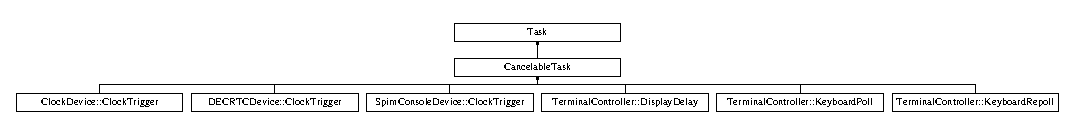
\includegraphics[height=1.27273cm]{classCancelableTask}
\end{center}
\end{figure}
\subsection*{Public Member Functions}
\begin{DoxyCompactItemize}
\item 
\hypertarget{classCancelableTask_a6b653553fe3e236d01128845d4c0fcdd}{
virtual void {\bfseries cancel} ()  throw ()}
\label{classCancelableTask_a6b653553fe3e236d01128845d4c0fcdd}

\item 
\hypertarget{classCancelableTask_a3f99478c88e6a5c171b6412ebb8e8a04}{
virtual void {\bfseries task} ()}
\label{classCancelableTask_a3f99478c88e6a5c171b6412ebb8e8a04}

\end{DoxyCompactItemize}
\subsection*{Protected Member Functions}
\begin{DoxyCompactItemize}
\item 
\hypertarget{classCancelableTask_adf2a0222f39d903f8a857797b6ebb912}{
virtual void {\bfseries real\_\-task} ()=0}
\label{classCancelableTask_adf2a0222f39d903f8a857797b6ebb912}

\end{DoxyCompactItemize}
\subsection*{Protected Attributes}
\begin{DoxyCompactItemize}
\item 
\hypertarget{classCancelableTask_a7aab83aa340cf5ca2156a62bc30f7ea0}{
bool {\bfseries needed}}
\label{classCancelableTask_a7aab83aa340cf5ca2156a62bc30f7ea0}

\end{DoxyCompactItemize}


The documentation for this class was generated from the following file:\begin{DoxyCompactItemize}
\item 
task.h\end{DoxyCompactItemize}

\hypertarget{classClock}{
\section{Clock Class Reference}
\label{classClock}\index{Clock@{Clock}}
}
\subsection*{Classes}
\begin{DoxyCompactItemize}
\item 
class \hyperlink{classClock_1_1DeferredTasks}{DeferredTasks}
\end{DoxyCompactItemize}
\subsection*{Public Member Functions}
\begin{DoxyCompactItemize}
\item 
\hypertarget{classClock_a52d72e9e9e8acd243bd0692b222898e5}{
{\bfseries Clock} (const timespec \&start\_\-time)  throw ()}
\label{classClock_a52d72e9e9e8acd243bd0692b222898e5}

\item 
\hypertarget{classClock_a4007cf9c21326281382a1f1244616e9d}{
virtual void {\bfseries increment\_\-time} (long nanoseconds)}
\label{classClock_a4007cf9c21326281382a1f1244616e9d}

\item 
\hypertarget{classClock_a1e102973afde24e2b1fc4f897976ce86}{
virtual void {\bfseries pass\_\-realtime} (uint32 timeratio)  throw ()}
\label{classClock_a1e102973afde24e2b1fc4f897976ce86}

\item 
\hypertarget{classClock_a78c89e7b78e718b21f4374eb84559d6f}{
virtual void {\bfseries add\_\-deferred\_\-task} (\hyperlink{classTask}{Task} $\ast$task, long nanoseconds)}
\label{classClock_a78c89e7b78e718b21f4374eb84559d6f}

\item 
\hypertarget{classClock_a97be7b0e631ff16e23d257bdbfd46bca}{
virtual timespec {\bfseries get\_\-time} ()  throw ()}
\label{classClock_a97be7b0e631ff16e23d257bdbfd46bca}

\item 
\hypertarget{classClock_a0c2cf0c2c990fe3e243d2ff1da458fa1}{
virtual void {\bfseries set\_\-time} (const timespec \&time)  throw ()}
\label{classClock_a0c2cf0c2c990fe3e243d2ff1da458fa1}

\end{DoxyCompactItemize}
\subsection*{Protected Attributes}
\begin{DoxyCompactItemize}
\item 
\hypertarget{classClock_a5bcbe67ab5e7401bb2aad2a404b9af73}{
timespec {\bfseries time}}
\label{classClock_a5bcbe67ab5e7401bb2aad2a404b9af73}

\item 
\hypertarget{classClock_a029c531061ff673036245dc49595929b}{
timespec {\bfseries then}}
\label{classClock_a029c531061ff673036245dc49595929b}

\item 
\hypertarget{classClock_a57d3bf1d0729b2595c55d9e3eb2df889}{
long {\bfseries spill\_\-ns}}
\label{classClock_a57d3bf1d0729b2595c55d9e3eb2df889}

\item 
\hypertarget{classClock_a6a93576eb5d034fc83fc631d2a436fd7}{
std::list$<$ \hyperlink{classClock_1_1DeferredTasks}{DeferredTasks} $\ast$ $>$ {\bfseries deferred\_\-tasks}}
\label{classClock_a6a93576eb5d034fc83fc631d2a436fd7}

\end{DoxyCompactItemize}


The documentation for this class was generated from the following files:\begin{DoxyCompactItemize}
\item 
clock.h\item 
clock.cc\end{DoxyCompactItemize}

\hypertarget{classClockDevice}{
\section{ClockDevice Class Reference}
\label{classClockDevice}\index{ClockDevice@{ClockDevice}}
}
Inheritance diagram for ClockDevice:\begin{figure}[H]
\begin{center}
\leavevmode
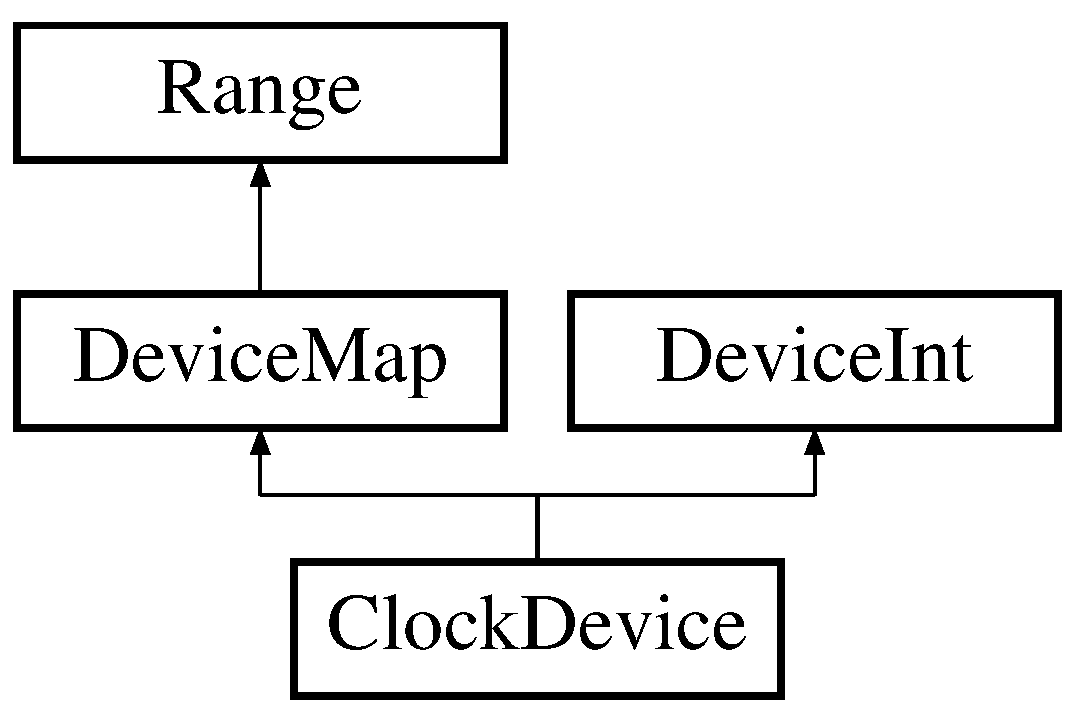
\includegraphics[height=3cm]{classClockDevice}
\end{center}
\end{figure}
\subsection*{Classes}
\begin{DoxyCompactItemize}
\item 
class \hyperlink{classClockDevice_1_1ClockTrigger}{ClockTrigger}
\end{DoxyCompactItemize}
\subsection*{Public Member Functions}
\begin{DoxyCompactItemize}
\item 
\hypertarget{classClockDevice_aba00ae8b6155e4b9e8570b8cbec432b6}{
{\bfseries ClockDevice} (\hyperlink{classClock}{Clock} $\ast$clock, uint32 irq, long frequency\_\-ns)  throw ( std::bad\_\-alloc )}
\label{classClockDevice_aba00ae8b6155e4b9e8570b8cbec432b6}

\item 
\hypertarget{classClockDevice_ac837bd6024524e14733fef9a3caf20bd}{
virtual void {\bfseries ready\_\-clock} ()  throw ( std::bad\_\-alloc )}
\label{classClockDevice_ac837bd6024524e14733fef9a3caf20bd}

\item 
\hypertarget{classClockDevice_a8fac0caef40e255d93162bdd0e2b0a63}{
virtual uint32 {\bfseries fetch\_\-word} (uint32 offset, int mode, \hyperlink{classDeviceExc}{DeviceExc} $\ast$client)}
\label{classClockDevice_a8fac0caef40e255d93162bdd0e2b0a63}

\item 
\hypertarget{classClockDevice_a87082836fc257de250ad4612ff50a281}{
virtual void {\bfseries store\_\-word} (uint32 offset, uint32 data, \hyperlink{classDeviceExc}{DeviceExc} $\ast$client)}
\label{classClockDevice_a87082836fc257de250ad4612ff50a281}

\item 
\hypertarget{classClockDevice_afb660217da1d9ce3142df8ffd04e6569}{
virtual const char $\ast$ {\bfseries descriptor\_\-str} () const }
\label{classClockDevice_afb660217da1d9ce3142df8ffd04e6569}

\end{DoxyCompactItemize}
\subsection*{Protected Types}
\begin{DoxyCompactItemize}
\item 
enum {\bfseries State} \{ {\bfseries UNREADY} =  0, 
{\bfseries READY} =  CTL\_\-RDY
 \}
\end{DoxyCompactItemize}
\subsection*{Protected Member Functions}
\begin{DoxyCompactItemize}
\item 
\hypertarget{classClockDevice_aad402cce484ce8c1fc8730029022a730}{
virtual void {\bfseries unready\_\-clock} ()  throw ()}
\label{classClockDevice_aad402cce484ce8c1fc8730029022a730}

\end{DoxyCompactItemize}
\subsection*{Protected Attributes}
\begin{DoxyCompactItemize}
\item 
\hypertarget{classClockDevice_a43d305efaa3b4ce21fec56209b77b936}{
const uint32 {\bfseries irq}}
\label{classClockDevice_a43d305efaa3b4ce21fec56209b77b936}

\item 
\hypertarget{classClockDevice_a0b398fdd22019bbac72426bcd035731b}{
const long {\bfseries frequency\_\-ns}}
\label{classClockDevice_a0b398fdd22019bbac72426bcd035731b}

\item 
\hypertarget{classClockDevice_a7d249ac5fcd2bab6dced445926363eaf}{
\hyperlink{classClock}{Clock} $\ast$ {\bfseries clock}}
\label{classClockDevice_a7d249ac5fcd2bab6dced445926363eaf}

\item 
\hypertarget{classClockDevice_a59429aef5d33a07cd1bf72ecb743c956}{
\hyperlink{classClockDevice_1_1ClockTrigger}{ClockTrigger} $\ast$ {\bfseries clock\_\-trigger}}
\label{classClockDevice_a59429aef5d33a07cd1bf72ecb743c956}

\item 
\hypertarget{classClockDevice_ac166cba15b49be2b29f3d6d7cd7da087}{
State {\bfseries clock\_\-state}}
\label{classClockDevice_ac166cba15b49be2b29f3d6d7cd7da087}

\item 
\hypertarget{classClockDevice_aee58d6b7d301a0791a511002d2ead157}{
bool {\bfseries interrupt\_\-enabled}}
\label{classClockDevice_aee58d6b7d301a0791a511002d2ead157}

\end{DoxyCompactItemize}


The documentation for this class was generated from the following files:\begin{DoxyCompactItemize}
\item 
clockdev.h\item 
clockdev.cc\end{DoxyCompactItemize}

\hypertarget{classClockDevice_1_1ClockTrigger}{
\section{ClockDevice::ClockTrigger Class Reference}
\label{classClockDevice_1_1ClockTrigger}\index{ClockDevice::ClockTrigger@{ClockDevice::ClockTrigger}}
}
Inheritance diagram for ClockDevice::ClockTrigger:\begin{figure}[H]
\begin{center}
\leavevmode
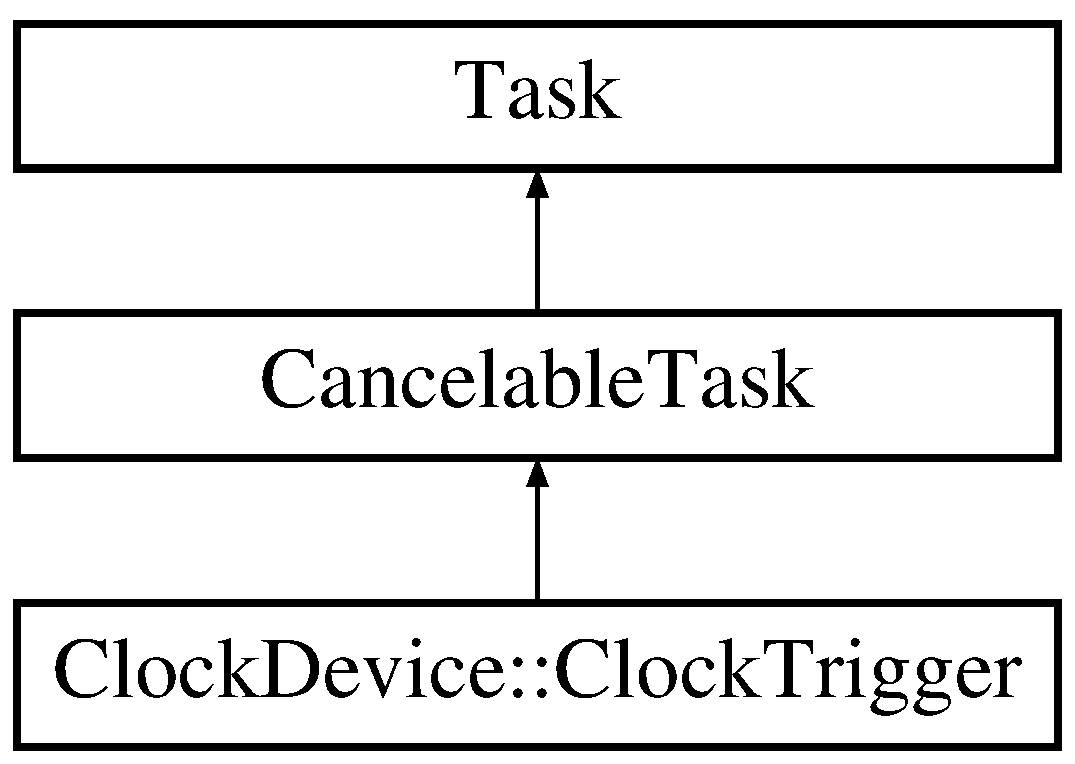
\includegraphics[height=3cm]{classClockDevice_1_1ClockTrigger}
\end{center}
\end{figure}
\subsection*{Public Member Functions}
\begin{DoxyCompactItemize}
\item 
\hypertarget{classClockDevice_1_1ClockTrigger_ab6f6e2ba478264425a68a0a8383e660a}{
{\bfseries ClockTrigger} (\hyperlink{classClockDevice}{ClockDevice} $\ast$clock\_\-device)  throw ()}
\label{classClockDevice_1_1ClockTrigger_ab6f6e2ba478264425a68a0a8383e660a}

\end{DoxyCompactItemize}
\subsection*{Protected Member Functions}
\begin{DoxyCompactItemize}
\item 
\hypertarget{classClockDevice_1_1ClockTrigger_af084d7bc8f88985fad96e49fd19f77bd}{
virtual void {\bfseries real\_\-task} ()}
\label{classClockDevice_1_1ClockTrigger_af084d7bc8f88985fad96e49fd19f77bd}

\end{DoxyCompactItemize}
\subsection*{Protected Attributes}
\begin{DoxyCompactItemize}
\item 
\hypertarget{classClockDevice_1_1ClockTrigger_ab7c5345ceeece045bebe2b40b4efdd96}{
\hyperlink{classClockDevice}{ClockDevice} $\ast$ {\bfseries clock\_\-device}}
\label{classClockDevice_1_1ClockTrigger_ab7c5345ceeece045bebe2b40b4efdd96}

\end{DoxyCompactItemize}


The documentation for this class was generated from the following files:\begin{DoxyCompactItemize}
\item 
clockdev.h\item 
clockdev.cc\end{DoxyCompactItemize}

\hypertarget{classDECRTCDevice_1_1ClockTrigger}{
\section{DECRTCDevice::ClockTrigger Class Reference}
\label{classDECRTCDevice_1_1ClockTrigger}\index{DECRTCDevice::ClockTrigger@{DECRTCDevice::ClockTrigger}}
}
Inheritance diagram for DECRTCDevice::ClockTrigger:\begin{figure}[H]
\begin{center}
\leavevmode
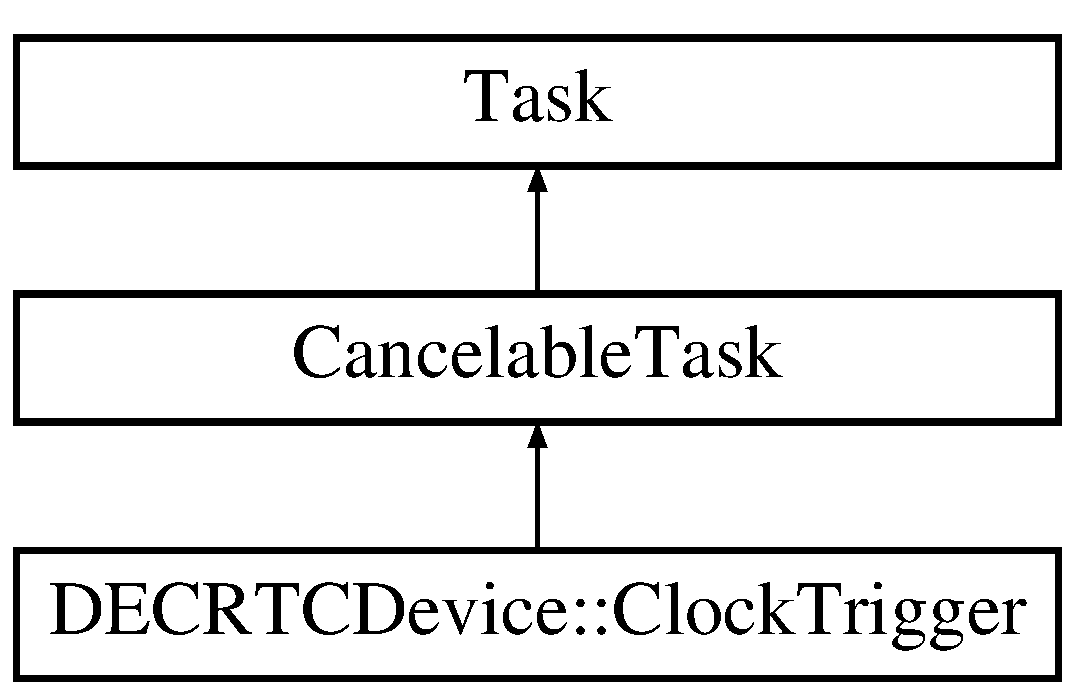
\includegraphics[height=3cm]{classDECRTCDevice_1_1ClockTrigger}
\end{center}
\end{figure}
\subsection*{Public Member Functions}
\begin{DoxyCompactItemize}
\item 
\hypertarget{classDECRTCDevice_1_1ClockTrigger_a91c8934e9b88f924764d8c36d9650b67}{
{\bfseries ClockTrigger} (\hyperlink{classDECRTCDevice}{DECRTCDevice} $\ast$rtc)  throw ()}
\label{classDECRTCDevice_1_1ClockTrigger_a91c8934e9b88f924764d8c36d9650b67}

\end{DoxyCompactItemize}
\subsection*{Protected Member Functions}
\begin{DoxyCompactItemize}
\item 
\hypertarget{classDECRTCDevice_1_1ClockTrigger_a0b2b3ae399edded5e6ac181dd6d7c66e}{
virtual void {\bfseries real\_\-task} ()}
\label{classDECRTCDevice_1_1ClockTrigger_a0b2b3ae399edded5e6ac181dd6d7c66e}

\end{DoxyCompactItemize}
\subsection*{Protected Attributes}
\begin{DoxyCompactItemize}
\item 
\hypertarget{classDECRTCDevice_1_1ClockTrigger_aeabc70cadfac9cabaa7d353c2befd3b4}{
\hyperlink{classDECRTCDevice}{DECRTCDevice} $\ast$ {\bfseries rtc}}
\label{classDECRTCDevice_1_1ClockTrigger_aeabc70cadfac9cabaa7d353c2befd3b4}

\end{DoxyCompactItemize}


The documentation for this class was generated from the following files:\begin{DoxyCompactItemize}
\item 
decrtc.h\item 
decrtc.cc\end{DoxyCompactItemize}

\hypertarget{classSpimConsoleDevice_1_1ClockTrigger}{
\section{SpimConsoleDevice::ClockTrigger Class Reference}
\label{classSpimConsoleDevice_1_1ClockTrigger}\index{SpimConsoleDevice::ClockTrigger@{SpimConsoleDevice::ClockTrigger}}
}
Inheritance diagram for SpimConsoleDevice::ClockTrigger:\begin{figure}[H]
\begin{center}
\leavevmode
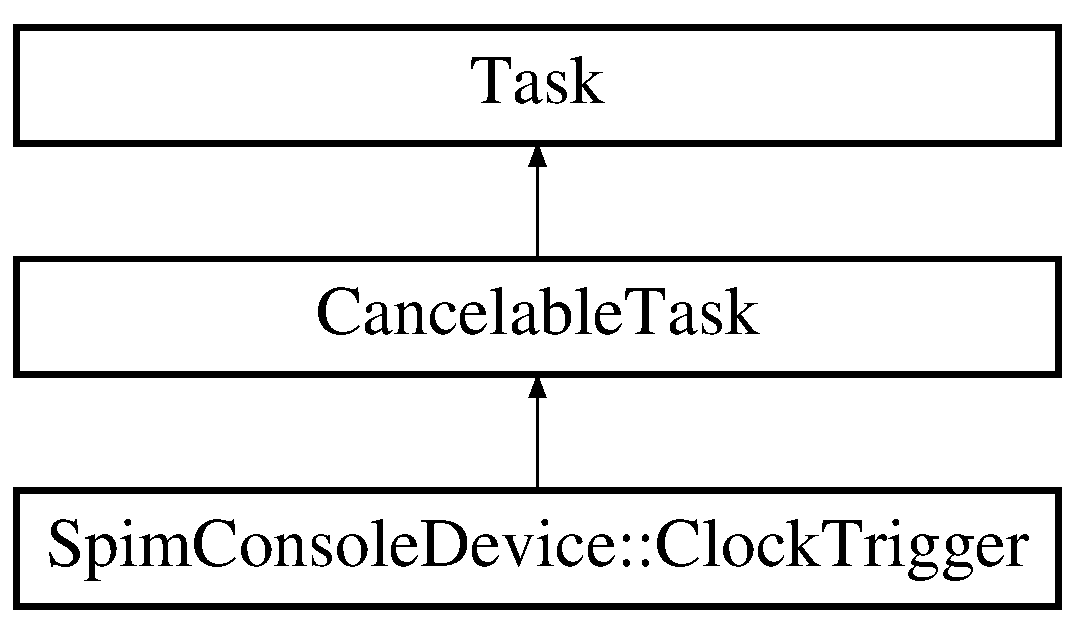
\includegraphics[height=3cm]{classSpimConsoleDevice_1_1ClockTrigger}
\end{center}
\end{figure}
\subsection*{Public Member Functions}
\begin{DoxyCompactItemize}
\item 
\hypertarget{classSpimConsoleDevice_1_1ClockTrigger_a1189607fbee809e8cf3270458a850ffc}{
{\bfseries ClockTrigger} (\hyperlink{classSpimConsoleDevice}{SpimConsoleDevice} $\ast$console)  throw ()}
\label{classSpimConsoleDevice_1_1ClockTrigger_a1189607fbee809e8cf3270458a850ffc}

\end{DoxyCompactItemize}
\subsection*{Protected Member Functions}
\begin{DoxyCompactItemize}
\item 
\hypertarget{classSpimConsoleDevice_1_1ClockTrigger_afa3ddbdd65d8500444b79cb4887f0f0e}{
virtual void {\bfseries real\_\-task} ()}
\label{classSpimConsoleDevice_1_1ClockTrigger_afa3ddbdd65d8500444b79cb4887f0f0e}

\end{DoxyCompactItemize}
\subsection*{Protected Attributes}
\begin{DoxyCompactItemize}
\item 
\hypertarget{classSpimConsoleDevice_1_1ClockTrigger_ad6f7ff2dd63d8b147ba4aab3bc28281c}{
\hyperlink{classSpimConsoleDevice}{SpimConsoleDevice} $\ast$ {\bfseries console}}
\label{classSpimConsoleDevice_1_1ClockTrigger_ad6f7ff2dd63d8b147ba4aab3bc28281c}

\end{DoxyCompactItemize}


The documentation for this class was generated from the following files:\begin{DoxyCompactItemize}
\item 
spimconsole.h\item 
spimconsole.cc\end{DoxyCompactItemize}

\hypertarget{structcoff__file__header}{
\section{coff\_\-file\_\-header Struct Reference}
\label{structcoff__file__header}\index{coff\_\-file\_\-header@{coff\_\-file\_\-header}}
}
\subsection*{Public Attributes}
\begin{DoxyCompactItemize}
\item 
\hypertarget{structcoff__file__header_af0ede941444cca81ca1015ebcfb3a63a}{
unsigned short {\bfseries magic}}
\label{structcoff__file__header_af0ede941444cca81ca1015ebcfb3a63a}

\item 
\hypertarget{structcoff__file__header_a9e71a1fee93bf716b0b87e14fe34f2d5}{
unsigned short {\bfseries no\_\-sections}}
\label{structcoff__file__header_a9e71a1fee93bf716b0b87e14fe34f2d5}

\item 
\hypertarget{structcoff__file__header_a693a1fd453de824f5327a0e29464867b}{
char {\bfseries extras} \mbox{[}20\mbox{]}}
\label{structcoff__file__header_a693a1fd453de824f5327a0e29464867b}

\item 
\hypertarget{structcoff__file__header_a4698d9c30e72e0943eb18b68c21a067c}{
unsigned long {\bfseries text\_\-size}}
\label{structcoff__file__header_a4698d9c30e72e0943eb18b68c21a067c}

\item 
\hypertarget{structcoff__file__header_a721f91dfdbd330fa01a181fe09657576}{
unsigned long {\bfseries data\_\-size}}
\label{structcoff__file__header_a721f91dfdbd330fa01a181fe09657576}

\item 
\hypertarget{structcoff__file__header_aa25757530dc4349808158515fe01ea0a}{
unsigned long {\bfseries bss\_\-size}}
\label{structcoff__file__header_aa25757530dc4349808158515fe01ea0a}

\item 
\hypertarget{structcoff__file__header_a824eee83be2037d48f8bc13362cf8b94}{
unsigned long {\bfseries entry\_\-addr}}
\label{structcoff__file__header_a824eee83be2037d48f8bc13362cf8b94}

\item 
\hypertarget{structcoff__file__header_a89e2d93abfe39040744e4cecee38b1db}{
unsigned long {\bfseries text\_\-start}}
\label{structcoff__file__header_a89e2d93abfe39040744e4cecee38b1db}

\item 
\hypertarget{structcoff__file__header_af8bf75aa92cf4079ba45a46d7c0d3b1c}{
unsigned long {\bfseries data\_\-start}}
\label{structcoff__file__header_af8bf75aa92cf4079ba45a46d7c0d3b1c}

\item 
\hypertarget{structcoff__file__header_ac7557f85ac4733028073dcdcab1e99a4}{
unsigned long {\bfseries bss\_\-start}}
\label{structcoff__file__header_ac7557f85ac4733028073dcdcab1e99a4}

\item 
\hypertarget{structcoff__file__header_a193e5699d76f0b4243bf268c9edae8df}{
char {\bfseries extras2} \mbox{[}20\mbox{]}}
\label{structcoff__file__header_a193e5699d76f0b4243bf268c9edae8df}

\item 
\hypertarget{structcoff__file__header_a103cd7f2a0cbc1134b930a5f5b84a82a}{
unsigned long {\bfseries gp\_\-value}}
\label{structcoff__file__header_a103cd7f2a0cbc1134b930a5f5b84a82a}

\end{DoxyCompactItemize}


The documentation for this struct was generated from the following file:\begin{DoxyCompactItemize}
\item 
exeloader.cc\end{DoxyCompactItemize}

\hypertarget{structcoff__info}{
\section{coff\_\-info Struct Reference}
\label{structcoff__info}\index{coff\_\-info@{coff\_\-info}}
}
\subsection*{Public Attributes}
\begin{DoxyCompactItemize}
\item 
\hypertarget{structcoff__info_ad6693cb0774b3b9a362049a0fdc4b14d}{
struct \hyperlink{structcoff__file__header}{coff\_\-file\_\-header} {\bfseries file\_\-header}}
\label{structcoff__info_ad6693cb0774b3b9a362049a0fdc4b14d}

\item 
\hypertarget{structcoff__info_a6cbe24985910403a898061fd8f09b325}{
unsigned long {\bfseries text\_\-addr}}
\label{structcoff__info_a6cbe24985910403a898061fd8f09b325}

\item 
\hypertarget{structcoff__info_aa9974d1ed5725878f3dc9c545163d45e}{
unsigned long {\bfseries text\_\-offset}}
\label{structcoff__info_aa9974d1ed5725878f3dc9c545163d45e}

\item 
\hypertarget{structcoff__info_ac9fe9564416b27391a61e3792ca62cc5}{
unsigned long {\bfseries text\_\-size}}
\label{structcoff__info_ac9fe9564416b27391a61e3792ca62cc5}

\item 
\hypertarget{structcoff__info_aac90a49e63ce4bb8f2c3c6dd5565290b}{
unsigned long {\bfseries data\_\-addr}}
\label{structcoff__info_aac90a49e63ce4bb8f2c3c6dd5565290b}

\item 
\hypertarget{structcoff__info_ad6888212f9aecd7d732f27a70d2e983d}{
unsigned long {\bfseries data\_\-offset}}
\label{structcoff__info_ad6888212f9aecd7d732f27a70d2e983d}

\item 
\hypertarget{structcoff__info_a985296bbaa2c7e5a2da7ebcc2ca70ae7}{
unsigned long {\bfseries data\_\-size}}
\label{structcoff__info_a985296bbaa2c7e5a2da7ebcc2ca70ae7}

\item 
\hypertarget{structcoff__info_a398603a664d7a43ab54b93cea5374802}{
unsigned long {\bfseries bss\_\-addr}}
\label{structcoff__info_a398603a664d7a43ab54b93cea5374802}

\item 
\hypertarget{structcoff__info_ae646d9e0c4d5215142a669a8ede686a7}{
unsigned long {\bfseries bss\_\-size}}
\label{structcoff__info_ae646d9e0c4d5215142a669a8ede686a7}

\end{DoxyCompactItemize}


The documentation for this struct was generated from the following file:\begin{DoxyCompactItemize}
\item 
exeloader.cc\end{DoxyCompactItemize}

\hypertarget{structcoff__section__header}{
\section{coff\_\-section\_\-header Struct Reference}
\label{structcoff__section__header}\index{coff\_\-section\_\-header@{coff\_\-section\_\-header}}
}
\subsection*{Public Attributes}
\begin{DoxyCompactItemize}
\item 
\hypertarget{structcoff__section__header_afd97540c559f1bb92df3c41a6484bea6}{
char {\bfseries section\_\-name} \mbox{[}8\mbox{]}}
\label{structcoff__section__header_afd97540c559f1bb92df3c41a6484bea6}

\item 
\hypertarget{structcoff__section__header_a23f345450c1f0a06ae535bae85712f22}{
unsigned long {\bfseries section\_\-phys\_\-addr}}
\label{structcoff__section__header_a23f345450c1f0a06ae535bae85712f22}

\item 
\hypertarget{structcoff__section__header_a308acfd379d401e4060ce5c0183964c0}{
unsigned long {\bfseries section\_\-virt\_\-addr}}
\label{structcoff__section__header_a308acfd379d401e4060ce5c0183964c0}

\item 
\hypertarget{structcoff__section__header_a2b3eca9648679d9118f1e869497e72a0}{
unsigned long {\bfseries section\_\-size}}
\label{structcoff__section__header_a2b3eca9648679d9118f1e869497e72a0}

\item 
\hypertarget{structcoff__section__header_a365990abf98c4d9e75bbb3def6bb647c}{
unsigned long {\bfseries section\_\-file\_\-loc}}
\label{structcoff__section__header_a365990abf98c4d9e75bbb3def6bb647c}

\item 
\hypertarget{structcoff__section__header_a3ae677fccda07e651da1d81186d857b4}{
char {\bfseries extras} \mbox{[}16\mbox{]}}
\label{structcoff__section__header_a3ae677fccda07e651da1d81186d857b4}

\end{DoxyCompactItemize}


The documentation for this struct was generated from the following file:\begin{DoxyCompactItemize}
\item 
exeloader.cc\end{DoxyCompactItemize}

\hypertarget{classPlog_1_1ConsoleRecorder}{
\section{Plog::ConsoleRecorder Class Reference}
\label{classPlog_1_1ConsoleRecorder}\index{Plog::ConsoleRecorder@{Plog::ConsoleRecorder}}
}
Inheritance diagram for Plog::ConsoleRecorder:\begin{figure}[H]
\begin{center}
\leavevmode
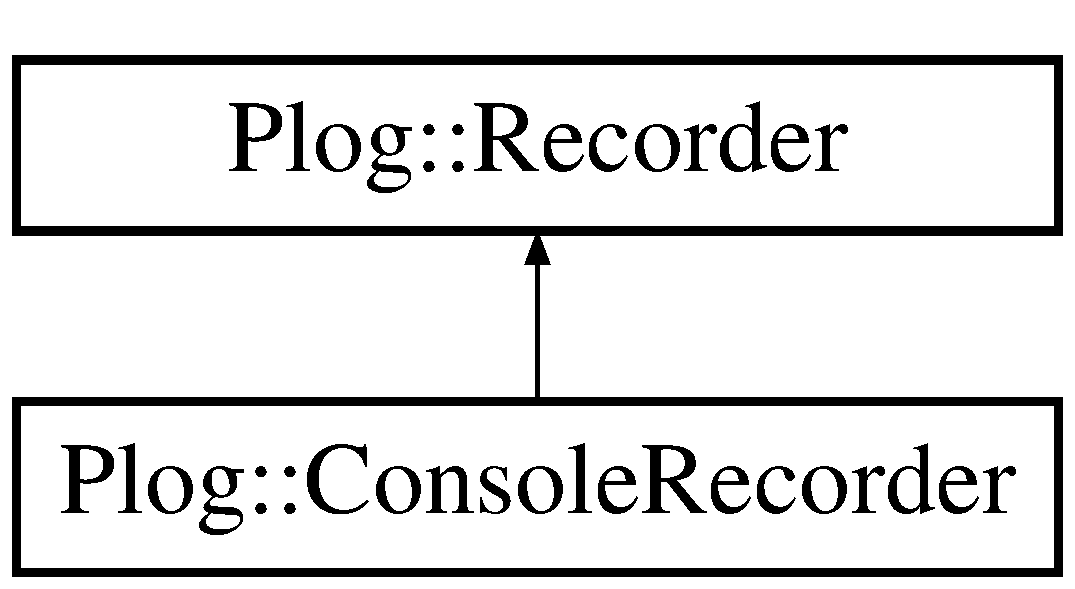
\includegraphics[height=2cm]{classPlog_1_1ConsoleRecorder}
\end{center}
\end{figure}
\subsection*{Public Member Functions}
\begin{DoxyCompactItemize}
\item 
\hypertarget{classPlog_1_1ConsoleRecorder_af898bdabf81b18ef3b7116e21be5dd83}{
virtual void {\bfseries RecordMessage} (Plog::PLOG\_\-LEVEL level, const std::string \&message)}
\label{classPlog_1_1ConsoleRecorder_af898bdabf81b18ef3b7116e21be5dd83}

\end{DoxyCompactItemize}


The documentation for this class was generated from the following file:\begin{DoxyCompactItemize}
\item 
prophetlog.cc\end{DoxyCompactItemize}

\hypertarget{structCponeClientData}{
\section{CponeClientData Struct Reference}
\label{structCponeClientData}\index{CponeClientData@{CponeClientData}}
}
\subsection*{Public Attributes}
\begin{DoxyCompactItemize}
\item 
\hypertarget{structCponeClientData_a8c00ff9b8dc855157e39c28153c63a3d}{
uint16 {\bfseries m\_\-rs}}
\label{structCponeClientData_a8c00ff9b8dc855157e39c28153c63a3d}

\item 
\hypertarget{structCponeClientData_a32ed256e83d863a90f15703ad5f1c939}{
uint16 {\bfseries m\_\-funct}}
\label{structCponeClientData_a32ed256e83d863a90f15703ad5f1c939}

\item 
\hypertarget{structCponeClientData_a0e766d5a2efdc208c2aca7187aa32af7}{
uint16 {\bfseries m\_\-ft}}
\label{structCponeClientData_a0e766d5a2efdc208c2aca7187aa32af7}

\end{DoxyCompactItemize}


The documentation for this struct was generated from the following file:\begin{DoxyCompactItemize}
\item 
prophetstatistic.h\end{DoxyCompactItemize}

\hypertarget{classCPU}{
\section{CPU Class Reference}
\label{classCPU}\index{CPU@{CPU}}
}
Inheritance diagram for CPU:\begin{figure}[H]
\begin{center}
\leavevmode
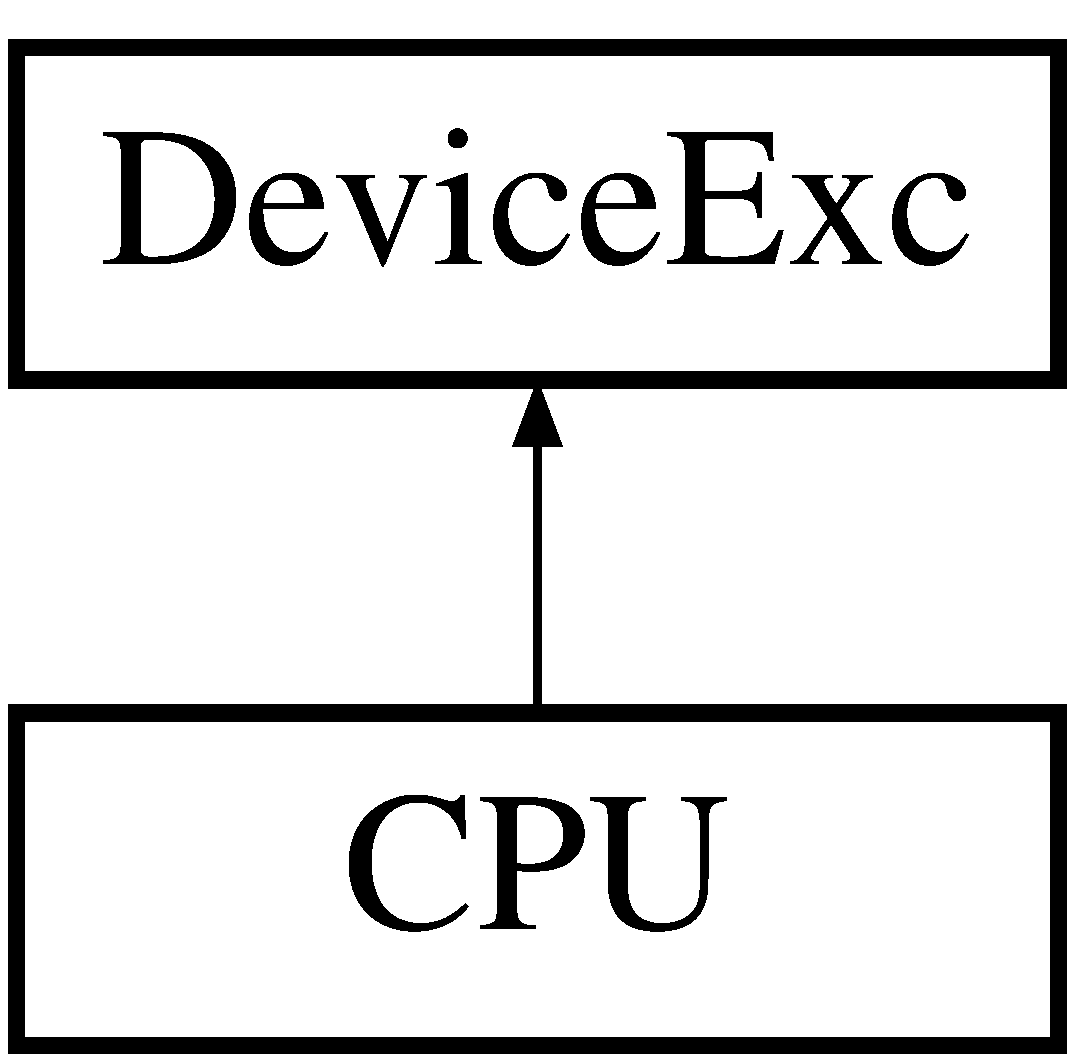
\includegraphics[height=2cm]{classCPU}
\end{center}
\end{figure}
\subsection*{Public Member Functions}
\begin{DoxyCompactItemize}
\item 
\hypertarget{classCPU_a7e03d573f476dd6b729afed1c7c9085c}{
uint16 {\bfseries opcode} (const uint32 instr) const }
\label{classCPU_a7e03d573f476dd6b729afed1c7c9085c}

\item 
\hypertarget{classCPU_a6a41d0dbc478e502ef7cb599e52a17cc}{
uint16 {\bfseries rs} (const uint32 instr) const }
\label{classCPU_a6a41d0dbc478e502ef7cb599e52a17cc}

\item 
\hypertarget{classCPU_a9697aa735fc4033872a5a6702e6fb60b}{
uint16 {\bfseries rt} (const uint32 instr) const }
\label{classCPU_a9697aa735fc4033872a5a6702e6fb60b}

\item 
\hypertarget{classCPU_a04e2dcd4a7db27fde59a4a8bad328aa3}{
uint16 {\bfseries rd} (const uint32 instr) const }
\label{classCPU_a04e2dcd4a7db27fde59a4a8bad328aa3}

\item 
\hypertarget{classCPU_a30a56a622f0b0330a0623cce118bfa57}{
uint16 {\bfseries immed} (const uint32 instr) const }
\label{classCPU_a30a56a622f0b0330a0623cce118bfa57}

\item 
\hypertarget{classCPU_a71d0d69f2f7099a062379c1fa464eb43}{
uint16 {\bfseries shamt} (const uint32 instr) const }
\label{classCPU_a71d0d69f2f7099a062379c1fa464eb43}

\item 
\hypertarget{classCPU_a8625d083f6783d5f7a46fce21f405441}{
uint16 {\bfseries funct} (const uint32 instr) const }
\label{classCPU_a8625d083f6783d5f7a46fce21f405441}

\item 
\hypertarget{classCPU_a442c4dff6234e6c2476d19c0cdd8fdab}{
uint32 {\bfseries jumptarg} (const uint32 instr) const }
\label{classCPU_a442c4dff6234e6c2476d19c0cdd8fdab}

\item 
\hypertarget{classCPU_a20fac2a174c994dc0e85e3896fab07f7}{
int16 {\bfseries s\_\-immed} (const uint32 instr) const }
\label{classCPU_a20fac2a174c994dc0e85e3896fab07f7}

\item 
\hypertarget{classCPU_a9545138874d05b828db69651ba74d04e}{
uint32 {\bfseries stacktop} () const }
\label{classCPU_a9545138874d05b828db69651ba74d04e}

\item 
\hypertarget{classCPU_a6b45c2cd1ca67d3a7a9af544c49628e8}{
{\bfseries CPU} (\hyperlink{classMapper}{Mapper} \&m, \hyperlink{classIntCtrl}{IntCtrl} \&i)}
\label{classCPU_a6b45c2cd1ca67d3a7a9af544c49628e8}

\item 
\hypertarget{classCPU_aaeb5869fd90b6462918d3d116332d8b5}{
virtual void {\bfseries dump\_\-regs} (FILE $\ast$f)}
\label{classCPU_aaeb5869fd90b6462918d3d116332d8b5}

\item 
\hypertarget{classCPU_ae24bbf9f230ba35d3d11d00e7e449dff}{
virtual void {\bfseries dump\_\-regs\_\-and\_\-stack} (FILE $\ast$f)}
\label{classCPU_ae24bbf9f230ba35d3d11d00e7e449dff}

\item 
\hypertarget{classCPU_af737d7d7d3c78fdae2e614787289ffad}{
virtual void {\bfseries cpzero\_\-dump\_\-regs\_\-and\_\-tlb} (FILE $\ast$f)}
\label{classCPU_af737d7d7d3c78fdae2e614787289ffad}

\item 
\hypertarget{classCPU_af4f84a4193a44aeef676abe4402b8c71}{
virtual void {\bfseries step} ()}
\label{classCPU_af4f84a4193a44aeef676abe4402b8c71}

\item 
\hypertarget{classCPU_acff6e2d8359b7ebea9153ea30b6c7596}{
char $\ast$const {\bfseries strexccode} (const uint16 excCode)}
\label{classCPU_acff6e2d8359b7ebea9153ea30b6c7596}

\item 
\hypertarget{classCPU_a7849dd448a89f9a7ca3f247ed2b9d757}{
char $\ast$const {\bfseries strdelaystate} (const int state)}
\label{classCPU_a7849dd448a89f9a7ca3f247ed2b9d757}

\item 
\hypertarget{classCPU_a5cc22e9cb5a61f8d0c2b226883974e15}{
char $\ast$const {\bfseries strmemmode} (const int memmode)}
\label{classCPU_a5cc22e9cb5a61f8d0c2b226883974e15}

\item 
\hypertarget{classCPU_a585862b2d962819486be215064fce20e}{
virtual void {\bfseries exception} (uint16 excCode, int mode=ANY, int coprocno=-\/1)}
\label{classCPU_a585862b2d962819486be215064fce20e}

\item 
\hypertarget{classCPU_a01e04d32f15a7812673db7fda78c3f33}{
virtual void {\bfseries reset} (void)}
\label{classCPU_a01e04d32f15a7812673db7fda78c3f33}

\item 
\hypertarget{classCPU_ae85238b9e47bee2df7a07eef2cba3e80}{
void {\bfseries maybe\_\-dump\_\-trace} ()}
\label{classCPU_ae85238b9e47bee2df7a07eef2cba3e80}

\item 
\hypertarget{classCPU_a7ab194fa6e72e7941646f095df76bff8}{
char $\ast$ {\bfseries debug\_\-registers\_\-to\_\-packet} (void)}
\label{classCPU_a7ab194fa6e72e7941646f095df76bff8}

\item 
\hypertarget{classCPU_a0fcea0002fb73af0ccdc07c8637b4020}{
void {\bfseries debug\_\-packet\_\-to\_\-registers} (char $\ast$packet)}
\label{classCPU_a0fcea0002fb73af0ccdc07c8637b4020}

\item 
\hypertarget{classCPU_a5be6cb440e54fb4f675fd9d6c1c1cb09}{
uint8 {\bfseries pending\_\-exception} (void)}
\label{classCPU_a5be6cb440e54fb4f675fd9d6c1c1cb09}

\item 
\hypertarget{classCPU_a9c56f582e6047ddd8bd2326c5af8d6f4}{
uint32 {\bfseries debug\_\-get\_\-pc} (void)}
\label{classCPU_a9c56f582e6047ddd8bd2326c5af8d6f4}

\item 
\hypertarget{classCPU_ae91c482028158094c67a9e3c626453e5}{
void {\bfseries debug\_\-set\_\-pc} (uint32 newpc)}
\label{classCPU_ae91c482028158094c67a9e3c626453e5}

\item 
\hypertarget{classCPU_a80b7efe3902cde8b1bab4849aa56d092}{
void {\bfseries debug\_\-packet\_\-push\_\-word} (char $\ast$packet, uint32 n)}
\label{classCPU_a80b7efe3902cde8b1bab4849aa56d092}

\item 
\hypertarget{classCPU_a8d2f406bc498ebe8a5f06c8461668c09}{
void {\bfseries debug\_\-packet\_\-push\_\-byte} (char $\ast$packet, uint8 n)}
\label{classCPU_a8d2f406bc498ebe8a5f06c8461668c09}

\item 
\hypertarget{classCPU_a7a38e0be35e2562521592c90170878fc}{
int {\bfseries debug\_\-fetch\_\-region} (uint32 addr, uint32 len, char $\ast$packet, \hyperlink{classDeviceExc}{DeviceExc} $\ast$client)}
\label{classCPU_a7a38e0be35e2562521592c90170878fc}

\item 
\hypertarget{classCPU_a19ccd19ddb57bcb4dfb13083a989bfe3}{
int {\bfseries debug\_\-store\_\-region} (uint32 addr, uint32 len, char $\ast$packet, \hyperlink{classDeviceExc}{DeviceExc} $\ast$client)}
\label{classCPU_a19ccd19ddb57bcb4dfb13083a989bfe3}

\end{DoxyCompactItemize}
\subsection*{Static Public Member Functions}
\begin{DoxyCompactItemize}
\item 
\hypertarget{classCPU_a801bca1865875594f3d36de6c0764cbb}{
static int32 {\bfseries srl} (int32, int32)}
\label{classCPU_a801bca1865875594f3d36de6c0764cbb}

\item 
\hypertarget{classCPU_a8e214a3b7f472087372e8dc826364304}{
static int32 {\bfseries sra} (int32, int32)}
\label{classCPU_a8e214a3b7f472087372e8dc826364304}

\end{DoxyCompactItemize}
\subsection*{Protected Member Functions}
\begin{DoxyCompactItemize}
\item 
\hypertarget{classCPU_ac7b1309543175ded1def959bee53bf5f}{
void {\bfseries start\_\-tracing} ()}
\label{classCPU_ac7b1309543175ded1def959bee53bf5f}

\item 
\hypertarget{classCPU_acd376de653b6c7bbf81fc3bb0e359563}{
void {\bfseries write\_\-trace\_\-to\_\-file} ()}
\label{classCPU_acd376de653b6c7bbf81fc3bb0e359563}

\item 
\hypertarget{classCPU_a16485b63e1e7ebf2344cf7f6f959f0ae}{
void {\bfseries write\_\-trace\_\-instr\_\-inputs} (uint32 instr)}
\label{classCPU_a16485b63e1e7ebf2344cf7f6f959f0ae}

\item 
\hypertarget{classCPU_afbaf48c07fa50fbe34921ae1d8fd1330}{
void {\bfseries write\_\-trace\_\-instr\_\-outputs} (uint32 instr)}
\label{classCPU_afbaf48c07fa50fbe34921ae1d8fd1330}

\item 
\hypertarget{classCPU_ac27e6471c16b2ef8db492741c378027d}{
void {\bfseries write\_\-trace\_\-record\_\-1} (uint32 pc, uint32 instr)}
\label{classCPU_ac27e6471c16b2ef8db492741c378027d}

\item 
\hypertarget{classCPU_ad4a6a675396f2e28d2ba597db7a046bb}{
void {\bfseries write\_\-trace\_\-record\_\-2} (uint32 pc, uint32 instr)}
\label{classCPU_ad4a6a675396f2e28d2ba597db7a046bb}

\item 
\hypertarget{classCPU_a4e7a051007781885d65efa15f178f04c}{
void {\bfseries stop\_\-tracing} ()}
\label{classCPU_a4e7a051007781885d65efa15f178f04c}

\item 
\hypertarget{classCPU_a3f626e9294073c7863592d0dc701556e}{
int {\bfseries exception\_\-priority} (uint16 excCode, int mode)}
\label{classCPU_a3f626e9294073c7863592d0dc701556e}

\item 
\hypertarget{classCPU_a634b14f9cd44bb7d9cdafe47944a354c}{
uint32 {\bfseries calc\_\-jump\_\-target} (uint32 instr, uint32 pc)}
\label{classCPU_a634b14f9cd44bb7d9cdafe47944a354c}

\item 
\hypertarget{classCPU_a3a8fb342dcef449afe2b7ee20841baf2}{
void {\bfseries branch} (uint32 instr, uint32 pc)}
\label{classCPU_a3a8fb342dcef449afe2b7ee20841baf2}

\item 
\hypertarget{classCPU_a4351cf31e0eaf15e424bdb33476f42e6}{
void {\bfseries mult64} (uint32 $\ast$hi, uint32 $\ast$lo, uint32 n, uint32 m)}
\label{classCPU_a4351cf31e0eaf15e424bdb33476f42e6}

\item 
\hypertarget{classCPU_a0c8fd1eb3a6ad3f2f33a637ff6f76f01}{
void {\bfseries mult64s} (uint32 $\ast$hi, uint32 $\ast$lo, int32 n, int32 m)}
\label{classCPU_a0c8fd1eb3a6ad3f2f33a637ff6f76f01}

\item 
\hypertarget{classCPU_a715c75aebed3ddb517d7435bce911b8b}{
void {\bfseries cop\_\-unimpl} (int coprocno, uint32 instr, uint32 pc)}
\label{classCPU_a715c75aebed3ddb517d7435bce911b8b}

\item 
\hypertarget{classCPU_a38aa633a220cd3b9fc704f4bb651b518}{
uint32 {\bfseries lwr} (uint32 regval, uint32 memval, uint8 offset)}
\label{classCPU_a38aa633a220cd3b9fc704f4bb651b518}

\item 
\hypertarget{classCPU_af19ad6fc54955e43d233a3c8c0d6eae8}{
uint32 {\bfseries lwl} (uint32 regval, uint32 memval, uint8 offset)}
\label{classCPU_af19ad6fc54955e43d233a3c8c0d6eae8}

\item 
\hypertarget{classCPU_a19ffe3daae5a78ce118f0e293e1e4a44}{
uint32 {\bfseries swl} (uint32 regval, uint32 memval, uint8 offset)}
\label{classCPU_a19ffe3daae5a78ce118f0e293e1e4a44}

\item 
\hypertarget{classCPU_aa1bcf3714f30fdcb8e7439396c7e60f8}{
uint32 {\bfseries swr} (uint32 regval, uint32 memval, uint8 offset)}
\label{classCPU_aa1bcf3714f30fdcb8e7439396c7e60f8}

\item 
\hypertarget{classCPU_a72d2375d4bda77bef899439c7f9b9b0f}{
virtual void {\bfseries funct\_\-emulate} (uint32 instr, uint32 pc)}
\label{classCPU_a72d2375d4bda77bef899439c7f9b9b0f}

\item 
\hypertarget{classCPU_a7f73382ebb68eeb29e5898f2088f3dbb}{
virtual void {\bfseries regimm\_\-emulate} (uint32 instr, uint32 pc)}
\label{classCPU_a7f73382ebb68eeb29e5898f2088f3dbb}

\item 
\hypertarget{classCPU_a6c941506a048425212cda8dff079a9c5}{
virtual void {\bfseries j\_\-emulate} (uint32 instr, uint32 pc)}
\label{classCPU_a6c941506a048425212cda8dff079a9c5}

\item 
\hypertarget{classCPU_aa65d0dc6f6e345d632d962cda7415ffc}{
virtual void {\bfseries jal\_\-emulate} (uint32 instr, uint32 pc)}
\label{classCPU_aa65d0dc6f6e345d632d962cda7415ffc}

\item 
\hypertarget{classCPU_ab8483602543bb291a6bcab1873226e6d}{
virtual void {\bfseries beq\_\-emulate} (uint32 instr, uint32 pc)}
\label{classCPU_ab8483602543bb291a6bcab1873226e6d}

\item 
\hypertarget{classCPU_ae1bbc7bdc294a982307db5dd92f3f29a}{
virtual void {\bfseries bne\_\-emulate} (uint32 instr, uint32 pc)}
\label{classCPU_ae1bbc7bdc294a982307db5dd92f3f29a}

\item 
\hypertarget{classCPU_a07d85530f9f0e3cd63d4e38e770c37df}{
virtual void {\bfseries blez\_\-emulate} (uint32 instr, uint32 pc)}
\label{classCPU_a07d85530f9f0e3cd63d4e38e770c37df}

\item 
\hypertarget{classCPU_ad099b433c0dd31578883fb7aab329c21}{
virtual void {\bfseries bgtz\_\-emulate} (uint32 instr, uint32 pc)}
\label{classCPU_ad099b433c0dd31578883fb7aab329c21}

\item 
\hypertarget{classCPU_ac59325c43ac5db28acdd841fc4755cc2}{
virtual void {\bfseries addi\_\-emulate} (uint32 instr, uint32 pc)}
\label{classCPU_ac59325c43ac5db28acdd841fc4755cc2}

\item 
\hypertarget{classCPU_adcf694d210e2340a1dcba7e1b1d8f147}{
virtual void {\bfseries addiu\_\-emulate} (uint32 instr, uint32 pc)}
\label{classCPU_adcf694d210e2340a1dcba7e1b1d8f147}

\item 
\hypertarget{classCPU_a6e6b0514f1ae4b8a92c5356bda7b6edc}{
virtual void {\bfseries slti\_\-emulate} (uint32 instr, uint32 pc)}
\label{classCPU_a6e6b0514f1ae4b8a92c5356bda7b6edc}

\item 
\hypertarget{classCPU_a7720b01681dae29df475f52a88d687d9}{
virtual void {\bfseries sltiu\_\-emulate} (uint32 instr, uint32 pc)}
\label{classCPU_a7720b01681dae29df475f52a88d687d9}

\item 
\hypertarget{classCPU_a428a65c6ca86430e3d5c34bae25aec4d}{
virtual void {\bfseries andi\_\-emulate} (uint32 instr, uint32 pc)}
\label{classCPU_a428a65c6ca86430e3d5c34bae25aec4d}

\item 
\hypertarget{classCPU_a881a19abc96daf5b3a010660f9f36e81}{
virtual void {\bfseries ori\_\-emulate} (uint32 instr, uint32 pc)}
\label{classCPU_a881a19abc96daf5b3a010660f9f36e81}

\item 
\hypertarget{classCPU_a76461399b3717c9feac047162f95824b}{
virtual void {\bfseries xori\_\-emulate} (uint32 instr, uint32 pc)}
\label{classCPU_a76461399b3717c9feac047162f95824b}

\item 
\hypertarget{classCPU_ab3bb4e55218c71542705abacc85cbbef}{
virtual void {\bfseries lui\_\-emulate} (uint32 instr, uint32 pc)}
\label{classCPU_ab3bb4e55218c71542705abacc85cbbef}

\item 
\hypertarget{classCPU_aab8c941ebf88267b842c8b63092c7df8}{
virtual void {\bfseries cpzero\_\-emulate} (uint32 instr, uint32 pc)}
\label{classCPU_aab8c941ebf88267b842c8b63092c7df8}

\item 
\hypertarget{classCPU_a221f6f3223e32a3b1f3b3d4c68628aac}{
virtual void {\bfseries cpone\_\-emulate} (uint32 instr, uint32 pc)}
\label{classCPU_a221f6f3223e32a3b1f3b3d4c68628aac}

\item 
\hypertarget{classCPU_ae338c1e5c3bc11c4f33bc7654b76edd4}{
virtual void {\bfseries cptwo\_\-emulate} (uint32 instr, uint32 pc)}
\label{classCPU_ae338c1e5c3bc11c4f33bc7654b76edd4}

\item 
\hypertarget{classCPU_a55223ec98f748ce379420d4eba934dbf}{
virtual void {\bfseries cpthree\_\-emulate} (uint32 instr, uint32 pc)}
\label{classCPU_a55223ec98f748ce379420d4eba934dbf}

\item 
\hypertarget{classCPU_a7f7353bd53ccdbd154658895ccb1790b}{
virtual void {\bfseries lb\_\-emulate} (uint32 instr, uint32 pc)}
\label{classCPU_a7f7353bd53ccdbd154658895ccb1790b}

\item 
\hypertarget{classCPU_a2431d002e82968109f1dc358c3e33ef7}{
virtual void {\bfseries lh\_\-emulate} (uint32 instr, uint32 pc)}
\label{classCPU_a2431d002e82968109f1dc358c3e33ef7}

\item 
\hypertarget{classCPU_ac1db353a9a93c7e47aa1f410bc23fec3}{
virtual void {\bfseries lwl\_\-emulate} (uint32 instr, uint32 pc)}
\label{classCPU_ac1db353a9a93c7e47aa1f410bc23fec3}

\item 
\hypertarget{classCPU_a0257d77024421e4c682789a1e981de02}{
virtual void {\bfseries lw\_\-emulate} (uint32 instr, uint32 pc)}
\label{classCPU_a0257d77024421e4c682789a1e981de02}

\item 
\hypertarget{classCPU_a784f872d9934535f849ca5533e6d2344}{
virtual void {\bfseries lbu\_\-emulate} (uint32 instr, uint32 pc)}
\label{classCPU_a784f872d9934535f849ca5533e6d2344}

\item 
\hypertarget{classCPU_a4fee10b21105794779b58964d69788bc}{
virtual void {\bfseries lhu\_\-emulate} (uint32 instr, uint32 pc)}
\label{classCPU_a4fee10b21105794779b58964d69788bc}

\item 
\hypertarget{classCPU_ae7a86c3813087678b5fef55d4b976400}{
virtual void {\bfseries lwr\_\-emulate} (uint32 instr, uint32 pc)}
\label{classCPU_ae7a86c3813087678b5fef55d4b976400}

\item 
\hypertarget{classCPU_a6399b7217b5d74860e5e815b0f36ec45}{
virtual void {\bfseries sb\_\-emulate} (uint32 instr, uint32 pc)}
\label{classCPU_a6399b7217b5d74860e5e815b0f36ec45}

\item 
\hypertarget{classCPU_afcdf6fb7c204c83a587efddbf16dea2e}{
virtual void {\bfseries sh\_\-emulate} (uint32 instr, uint32 pc)}
\label{classCPU_afcdf6fb7c204c83a587efddbf16dea2e}

\item 
\hypertarget{classCPU_ad6e88cf043663ae4d8e72e3bc16ba52d}{
virtual void {\bfseries swl\_\-emulate} (uint32 instr, uint32 pc)}
\label{classCPU_ad6e88cf043663ae4d8e72e3bc16ba52d}

\item 
\hypertarget{classCPU_a4360afbe04f87387ad1d43f7904548da}{
virtual void {\bfseries sw\_\-emulate} (uint32 instr, uint32 pc)}
\label{classCPU_a4360afbe04f87387ad1d43f7904548da}

\item 
\hypertarget{classCPU_a6c8501261f20dbfd3d1b62c63ab8b75b}{
virtual void {\bfseries swr\_\-emulate} (uint32 instr, uint32 pc)}
\label{classCPU_a6c8501261f20dbfd3d1b62c63ab8b75b}

\item 
\hypertarget{classCPU_acc036fc3519f4f57491748a374ea53a4}{
virtual void {\bfseries lwc1\_\-emulate} (uint32 instr, uint32 pc)}
\label{classCPU_acc036fc3519f4f57491748a374ea53a4}

\item 
\hypertarget{classCPU_ab970502c538f46c135abdd5f4de9b81a}{
virtual void {\bfseries lwc2\_\-emulate} (uint32 instr, uint32 pc)}
\label{classCPU_ab970502c538f46c135abdd5f4de9b81a}

\item 
\hypertarget{classCPU_afd81fbeb5e17dfd25d9179bdc7d14db7}{
virtual void {\bfseries lwc3\_\-emulate} (uint32 instr, uint32 pc)}
\label{classCPU_afd81fbeb5e17dfd25d9179bdc7d14db7}

\item 
\hypertarget{classCPU_ad870b60115457a544ea3a918d8857ff1}{
virtual void {\bfseries swc1\_\-emulate} (uint32 instr, uint32 pc)}
\label{classCPU_ad870b60115457a544ea3a918d8857ff1}

\item 
\hypertarget{classCPU_a865e0b2b102058612e50e881cba1d2c2}{
virtual void {\bfseries swc2\_\-emulate} (uint32 instr, uint32 pc)}
\label{classCPU_a865e0b2b102058612e50e881cba1d2c2}

\item 
\hypertarget{classCPU_a203756a36c870eb6a021e4b973aaa323}{
virtual void {\bfseries swc3\_\-emulate} (uint32 instr, uint32 pc)}
\label{classCPU_a203756a36c870eb6a021e4b973aaa323}

\item 
\hypertarget{classCPU_aad350e5ee056964fd731a202cc78bd89}{
virtual void {\bfseries sll\_\-emulate} (uint32 instr, uint32 pc)}
\label{classCPU_aad350e5ee056964fd731a202cc78bd89}

\item 
\hypertarget{classCPU_ac64c37e5dfdb289b3afd52edc2d149da}{
virtual void {\bfseries srl\_\-emulate} (uint32 instr, uint32 pc)}
\label{classCPU_ac64c37e5dfdb289b3afd52edc2d149da}

\item 
\hypertarget{classCPU_a741bf7a0064e8537e6b2928a87d884f7}{
virtual void {\bfseries sra\_\-emulate} (uint32 instr, uint32 pc)}
\label{classCPU_a741bf7a0064e8537e6b2928a87d884f7}

\item 
\hypertarget{classCPU_a70107be5ef7958b4f8dcb16dc6afb508}{
virtual void {\bfseries sllv\_\-emulate} (uint32 instr, uint32 pc)}
\label{classCPU_a70107be5ef7958b4f8dcb16dc6afb508}

\item 
\hypertarget{classCPU_a381d274b6a98e34bee7eaee59b9fcb25}{
virtual void {\bfseries srlv\_\-emulate} (uint32 instr, uint32 pc)}
\label{classCPU_a381d274b6a98e34bee7eaee59b9fcb25}

\item 
\hypertarget{classCPU_ad9cfbc8582d0e893f7f651c7d5862681}{
virtual void {\bfseries srav\_\-emulate} (uint32 instr, uint32 pc)}
\label{classCPU_ad9cfbc8582d0e893f7f651c7d5862681}

\item 
\hypertarget{classCPU_a4f76c106a8442177c26c4d9e8f21ab00}{
virtual void {\bfseries jr\_\-emulate} (uint32 instr, uint32 pc)}
\label{classCPU_a4f76c106a8442177c26c4d9e8f21ab00}

\item 
\hypertarget{classCPU_ac8473a1739c9f36114c17ca090c96029}{
virtual void {\bfseries jalr\_\-emulate} (uint32 instr, uint32 pc)}
\label{classCPU_ac8473a1739c9f36114c17ca090c96029}

\item 
\hypertarget{classCPU_a69221569c1d91b9846ff0b7298b1ed0a}{
virtual void {\bfseries syscall\_\-emulate} (uint32 instr, uint32 pc)}
\label{classCPU_a69221569c1d91b9846ff0b7298b1ed0a}

\item 
\hypertarget{classCPU_a995494b1b1fd54168872ca4f42b29660}{
virtual void {\bfseries break\_\-emulate} (uint32 instr, uint32 pc)}
\label{classCPU_a995494b1b1fd54168872ca4f42b29660}

\item 
\hypertarget{classCPU_a8da9a59554ff9a53472709ee814e74e0}{
virtual void {\bfseries mfhi\_\-emulate} (uint32 instr, uint32 pc)}
\label{classCPU_a8da9a59554ff9a53472709ee814e74e0}

\item 
\hypertarget{classCPU_a64b4ec5e152118af94b96d6d4c91fe17}{
virtual void {\bfseries mthi\_\-emulate} (uint32 instr, uint32 pc)}
\label{classCPU_a64b4ec5e152118af94b96d6d4c91fe17}

\item 
\hypertarget{classCPU_a2d07b1303a8304c8735a73303e8d5910}{
virtual void {\bfseries mflo\_\-emulate} (uint32 instr, uint32 pc)}
\label{classCPU_a2d07b1303a8304c8735a73303e8d5910}

\item 
\hypertarget{classCPU_ae3c368a547d34fc80304e37803b72aa4}{
virtual void {\bfseries mtlo\_\-emulate} (uint32 instr, uint32 pc)}
\label{classCPU_ae3c368a547d34fc80304e37803b72aa4}

\item 
\hypertarget{classCPU_a647a5f5891972fd74c5890912a8555c0}{
virtual void {\bfseries mult\_\-emulate} (uint32 instr, uint32 pc)}
\label{classCPU_a647a5f5891972fd74c5890912a8555c0}

\item 
\hypertarget{classCPU_af8628854d517536beef3881efe38fd49}{
virtual void {\bfseries multu\_\-emulate} (uint32 instr, uint32 pc)}
\label{classCPU_af8628854d517536beef3881efe38fd49}

\item 
\hypertarget{classCPU_ab95168699ff1d7584235ee5c809f44b1}{
virtual void {\bfseries div\_\-emulate} (uint32 instr, uint32 pc)}
\label{classCPU_ab95168699ff1d7584235ee5c809f44b1}

\item 
\hypertarget{classCPU_a2b590f2e5e763f6da34d0fcea9e7c8f9}{
virtual void {\bfseries divu\_\-emulate} (uint32 instr, uint32 pc)}
\label{classCPU_a2b590f2e5e763f6da34d0fcea9e7c8f9}

\item 
\hypertarget{classCPU_ad0484160ae69b0ac2846b1b3b0b1999c}{
virtual void {\bfseries add\_\-emulate} (uint32 instr, uint32 pc)}
\label{classCPU_ad0484160ae69b0ac2846b1b3b0b1999c}

\item 
\hypertarget{classCPU_ab3e34c227c2b9fdedb4864bff4b74b58}{
virtual void {\bfseries addu\_\-emulate} (uint32 instr, uint32 pc)}
\label{classCPU_ab3e34c227c2b9fdedb4864bff4b74b58}

\item 
\hypertarget{classCPU_a2068ff82e63f8cc9d1c592bf43beb136}{
virtual void {\bfseries sub\_\-emulate} (uint32 instr, uint32 pc)}
\label{classCPU_a2068ff82e63f8cc9d1c592bf43beb136}

\item 
\hypertarget{classCPU_a021ea426761c59fa7ffcfbcd4e66a645}{
virtual void {\bfseries subu\_\-emulate} (uint32 instr, uint32 pc)}
\label{classCPU_a021ea426761c59fa7ffcfbcd4e66a645}

\item 
\hypertarget{classCPU_a692f230fa6a061aea3c841c7370f6d1c}{
virtual void {\bfseries and\_\-emulate} (uint32 instr, uint32 pc)}
\label{classCPU_a692f230fa6a061aea3c841c7370f6d1c}

\item 
\hypertarget{classCPU_aafea7d93d1b958836509d66dd0e7076a}{
virtual void {\bfseries or\_\-emulate} (uint32 instr, uint32 pc)}
\label{classCPU_aafea7d93d1b958836509d66dd0e7076a}

\item 
\hypertarget{classCPU_a1ba85e418ee61a271a9aafbfde3351d7}{
virtual void {\bfseries xor\_\-emulate} (uint32 instr, uint32 pc)}
\label{classCPU_a1ba85e418ee61a271a9aafbfde3351d7}

\item 
\hypertarget{classCPU_a083835bce0c15e35ca834d0a0ecf2d22}{
virtual void {\bfseries nor\_\-emulate} (uint32 instr, uint32 pc)}
\label{classCPU_a083835bce0c15e35ca834d0a0ecf2d22}

\item 
\hypertarget{classCPU_a559d3f67d5b4119fe3fd595132a5185e}{
virtual void {\bfseries slt\_\-emulate} (uint32 instr, uint32 pc)}
\label{classCPU_a559d3f67d5b4119fe3fd595132a5185e}

\item 
\hypertarget{classCPU_ab96315f07f7fa574462e490bfdcfab3a}{
virtual void {\bfseries sltu\_\-emulate} (uint32 instr, uint32 pc)}
\label{classCPU_ab96315f07f7fa574462e490bfdcfab3a}

\item 
\hypertarget{classCPU_a646c50f8a1c19a8969417b746006a858}{
virtual void {\bfseries bltz\_\-emulate} (uint32 instr, uint32 pc)}
\label{classCPU_a646c50f8a1c19a8969417b746006a858}

\item 
\hypertarget{classCPU_a2a254799bd1e3545a1ec4d0cb65bb46e}{
virtual void {\bfseries bgez\_\-emulate} (uint32 instr, uint32 pc)}
\label{classCPU_a2a254799bd1e3545a1ec4d0cb65bb46e}

\item 
\hypertarget{classCPU_aff3e31b1a382ffc29f1ac7ba522735d8}{
virtual void {\bfseries bltzal\_\-emulate} (uint32 instr, uint32 pc)}
\label{classCPU_aff3e31b1a382ffc29f1ac7ba522735d8}

\item 
\hypertarget{classCPU_a14fa3b5c3dd0d71e36a71d7d3615cac9}{
virtual void {\bfseries bgezal\_\-emulate} (uint32 instr, uint32 pc)}
\label{classCPU_a14fa3b5c3dd0d71e36a71d7d3615cac9}

\item 
\hypertarget{classCPU_a2220cac151f1745874a46eed35761ddb}{
virtual void {\bfseries RI\_\-emulate} (uint32 instr, uint32 pc)}
\label{classCPU_a2220cac151f1745874a46eed35761ddb}

\end{DoxyCompactItemize}
\subsection*{Protected Attributes}
\begin{DoxyCompactItemize}
\item 
\hypertarget{classCPU_a30e8bf76edeea76f1f19a3bf7588f08a}{
bool {\bfseries tracing}}
\label{classCPU_a30e8bf76edeea76f1f19a3bf7588f08a}

\item 
\hypertarget{classCPU_acf034d26af3bd99a779aa8cb03e4670b}{
\hyperlink{classTrace}{Trace} {\bfseries current\_\-trace}}
\label{classCPU_acf034d26af3bd99a779aa8cb03e4670b}

\item 
\hypertarget{classCPU_a07aec7e8072099db8530d76af2335014}{
\hyperlink{structTrace_1_1Record}{Trace::Record} {\bfseries current\_\-trace\_\-record}}
\label{classCPU_a07aec7e8072099db8530d76af2335014}

\item 
\hypertarget{classCPU_a814367f222141355ec6deb579b6f0c58}{
uint32 {\bfseries pc}}
\label{classCPU_a814367f222141355ec6deb579b6f0c58}

\item 
\hypertarget{classCPU_a2a203ccf5813098e0dbedff0e47a76d3}{
uint32 {\bfseries reg} \mbox{[}CPU\_\-REG\_\-NUMBER\mbox{]}}
\label{classCPU_a2a203ccf5813098e0dbedff0e47a76d3}

\item 
\hypertarget{classCPU_ad754b47111e41660a7707bf0002bfa76}{
uint32 {\bfseries instr}}
\label{classCPU_ad754b47111e41660a7707bf0002bfa76}

\item 
\hypertarget{classCPU_af3f7d0decfadf0044fca99c868108055}{
uint32 {\bfseries hi}}
\label{classCPU_af3f7d0decfadf0044fca99c868108055}

\item 
\hypertarget{classCPU_a0ae013325ebf52209475496f1e45264d}{
uint32 {\bfseries lo}}
\label{classCPU_a0ae013325ebf52209475496f1e45264d}

\item 
\hypertarget{classCPU_a9474f06e26d535fb212ca3b594729214}{
uint32 {\bfseries last\_\-epc}}
\label{classCPU_a9474f06e26d535fb212ca3b594729214}

\item 
\hypertarget{classCPU_a5e994b9bd7c9e4cdd9f96c05b8628508}{
int {\bfseries last\_\-prio}}
\label{classCPU_a5e994b9bd7c9e4cdd9f96c05b8628508}

\item 
\hypertarget{classCPU_a6c4ebc6669d7ae0a967877f71edba69a}{
uint32 {\bfseries next\_\-epc}}
\label{classCPU_a6c4ebc6669d7ae0a967877f71edba69a}

\item 
\hypertarget{classCPU_ab29063010314e2c43e895175dcaa5da8}{
\hyperlink{classMapper}{Mapper} $\ast$ {\bfseries mem}}
\label{classCPU_ab29063010314e2c43e895175dcaa5da8}

\item 
\hypertarget{classCPU_ad63e0dcf43cf8203364537060f74f606}{
\hyperlink{classCPZero}{CPZero} $\ast$ {\bfseries cpzero}}
\label{classCPU_ad63e0dcf43cf8203364537060f74f606}

\item 
\hypertarget{classCPU_afce2b5a5943b8c065445c5c42a838a7a}{
int {\bfseries delay\_\-state}}
\label{classCPU_afce2b5a5943b8c065445c5c42a838a7a}

\item 
\hypertarget{classCPU_ae574769b3080a6e127e1cd4c197aca24}{
uint32 {\bfseries delay\_\-pc}}
\label{classCPU_ae574769b3080a6e127e1cd4c197aca24}

\item 
\hypertarget{classCPU_ab0d52929cc1df68657aba325d6e54316}{
bool {\bfseries opt\_\-excmsg}}
\label{classCPU_ab0d52929cc1df68657aba325d6e54316}

\item 
\hypertarget{classCPU_a1af3a29649ffaa317ada183a9d4cf5e6}{
bool {\bfseries opt\_\-reportirq}}
\label{classCPU_a1af3a29649ffaa317ada183a9d4cf5e6}

\item 
\hypertarget{classCPU_a5beb05958a1b9f3a1fdb22ce76ec5eb3}{
bool {\bfseries opt\_\-excpriomsg}}
\label{classCPU_a5beb05958a1b9f3a1fdb22ce76ec5eb3}

\item 
\hypertarget{classCPU_a0ba7f30aa285d7dce17cbe1e7aceade3}{
bool {\bfseries opt\_\-haltbreak}}
\label{classCPU_a0ba7f30aa285d7dce17cbe1e7aceade3}

\item 
\hypertarget{classCPU_a2c30e69ecfc26798e226c3393dfbc00a}{
bool {\bfseries opt\_\-haltibe}}
\label{classCPU_a2c30e69ecfc26798e226c3393dfbc00a}

\item 
\hypertarget{classCPU_a6143c857e05b425ac338f02bec98acc9}{
bool {\bfseries opt\_\-haltjrra}}
\label{classCPU_a6143c857e05b425ac338f02bec98acc9}

\item 
\hypertarget{classCPU_ac110631313f904bec3a220d09ff2059e}{
bool {\bfseries opt\_\-instdump}}
\label{classCPU_ac110631313f904bec3a220d09ff2059e}

\item 
\hypertarget{classCPU_a71cb0088ee9232425f0d91b2515e63c7}{
bool {\bfseries opt\_\-tracing}}
\label{classCPU_a71cb0088ee9232425f0d91b2515e63c7}

\item 
\hypertarget{classCPU_ad4b5995ace46f91553d1587748bce505}{
uint32 {\bfseries opt\_\-tracesize}}
\label{classCPU_ad4b5995ace46f91553d1587748bce505}

\item 
\hypertarget{classCPU_af9bf7995b16fdb0835c5ab6b6ab615d5}{
uint32 {\bfseries opt\_\-tracestartpc}}
\label{classCPU_af9bf7995b16fdb0835c5ab6b6ab615d5}

\item 
\hypertarget{classCPU_a9f48aa68d5317676ff8f433fe5605149}{
uint32 {\bfseries opt\_\-traceendpc}}
\label{classCPU_a9f48aa68d5317676ff8f433fe5605149}

\item 
\hypertarget{classCPU_a72f0d1686f2261398e815a9e5658de69}{
bool {\bfseries opt\_\-bigendian}}
\label{classCPU_a72f0d1686f2261398e815a9e5658de69}

\end{DoxyCompactItemize}
\subsection*{Friends}
\begin{DoxyCompactItemize}
\item 
\hypertarget{classCPU_ae03ffac5ee6974e43cec96baf6063c70}{
class \hyperlink{classCPU_ae03ffac5ee6974e43cec96baf6063c70}{CPZero}}
\label{classCPU_ae03ffac5ee6974e43cec96baf6063c70}

\end{DoxyCompactItemize}


The documentation for this class was generated from the following files:\begin{DoxyCompactItemize}
\item 
cpu.h\item 
cpu.cc\end{DoxyCompactItemize}

\hypertarget{classCPZero}{
\section{CPZero Class Reference}
\label{classCPZero}\index{CPZero@{CPZero}}
}
\subsection*{Public Member Functions}
\begin{DoxyCompactItemize}
\item 
\hypertarget{classCPZero_a703d4b95b23ecfc4039ec1001b706e0c}{
void {\bfseries tlb\_\-write} (unsigned index)}
\label{classCPZero_a703d4b95b23ecfc4039ec1001b706e0c}

\item 
\hypertarget{classCPZero_a3bcb604871913be1e6ab8fa917f794fe}{
uint32 {\bfseries read\_\-reg} (uint32 reg)}
\label{classCPZero_a3bcb604871913be1e6ab8fa917f794fe}

\item 
\hypertarget{classCPZero_ae9a4cd90b9983d4958862df5a9e944c8}{
void {\bfseries write\_\-reg} (uint32 reg, uint32 data)}
\label{classCPZero_ae9a4cd90b9983d4958862df5a9e944c8}

\item 
\hypertarget{classCPZero_a105d64ef00d18f173425ca16172f140b}{
bool {\bfseries cpCond} ()}
\label{classCPZero_a105d64ef00d18f173425ca16172f140b}

\item 
\hypertarget{classCPZero_a1c0dc92c666aaa4b420990693aad289f}{
{\bfseries CPZero} (\hyperlink{classCPU}{CPU} $\ast$m, \hyperlink{classIntCtrl}{IntCtrl} $\ast$i)}
\label{classCPZero_a1c0dc92c666aaa4b420990693aad289f}

\item 
\hypertarget{classCPZero_a53c439f8991ed00861eea4bdf567d719}{
void {\bfseries reset} (void)}
\label{classCPZero_a53c439f8991ed00861eea4bdf567d719}

\item 
\hypertarget{classCPZero_a68d1b7345c9504dd6c3558167bf2f7fd}{
uint32 {\bfseries address\_\-trans} (uint32 vaddr, int mode, bool $\ast$cacheable, \hyperlink{classDeviceExc}{DeviceExc} $\ast$client)}
\label{classCPZero_a68d1b7345c9504dd6c3558167bf2f7fd}

\item 
\hypertarget{classCPZero_a578fcf97eaf38f17b7fbaf39ccb8c517}{
void {\bfseries enter\_\-exception} (uint32 pc, uint32 excCode, uint32 ce, bool dly)}
\label{classCPZero_a578fcf97eaf38f17b7fbaf39ccb8c517}

\item 
\hypertarget{classCPZero_a92925ab954e16699c7cf01b934487927}{
bool {\bfseries use\_\-boot\_\-excp\_\-address} (void)}
\label{classCPZero_a92925ab954e16699c7cf01b934487927}

\item 
\hypertarget{classCPZero_ad27c7ba8138729180ed38c237788b8a4}{
bool {\bfseries caches\_\-isolated} (void)}
\label{classCPZero_ad27c7ba8138729180ed38c237788b8a4}

\item 
\hypertarget{classCPZero_a11fbfd1f5f3580e12590e0db1a52b0ce}{
bool {\bfseries caches\_\-swapped} (void)}
\label{classCPZero_a11fbfd1f5f3580e12590e0db1a52b0ce}

\item 
\hypertarget{classCPZero_afc99ae5fbd2e3e32f6982d10da788513}{
bool {\bfseries cop\_\-usable} (int coprocno)}
\label{classCPZero_afc99ae5fbd2e3e32f6982d10da788513}

\item 
\hypertarget{classCPZero_a177170b3404aca7a1adf655b22d06ef0}{
void {\bfseries cpzero\_\-emulate} (uint32 instr, uint32 pc)}
\label{classCPZero_a177170b3404aca7a1adf655b22d06ef0}

\item 
\hypertarget{classCPZero_aee1b391ace97d07fcd551133a6725ac2}{
void {\bfseries dump\_\-regs} (FILE $\ast$f)}
\label{classCPZero_aee1b391ace97d07fcd551133a6725ac2}

\item 
\hypertarget{classCPZero_a7b1425b75a48855fe10c88a7a01eab26}{
void {\bfseries dump\_\-tlb} (FILE $\ast$f)}
\label{classCPZero_a7b1425b75a48855fe10c88a7a01eab26}

\item 
\hypertarget{classCPZero_a2bf7aa14a71d8ae4ffb4a3f9c352e971}{
void {\bfseries dump\_\-regs\_\-and\_\-tlb} (FILE $\ast$f)}
\label{classCPZero_a2bf7aa14a71d8ae4ffb4a3f9c352e971}

\item 
\hypertarget{classCPZero_a343f7ad989439421dd250c1a81d37d4c}{
void {\bfseries adjust\_\-random} (void)}
\label{classCPZero_a343f7ad989439421dd250c1a81d37d4c}

\item 
\hypertarget{classCPZero_a566560627c3f4fab281a63944bf9ffc1}{
bool {\bfseries interrupt\_\-pending} (void)}
\label{classCPZero_a566560627c3f4fab281a63944bf9ffc1}

\item 
\hypertarget{classCPZero_a57001ba4feae636ec47c8b6593e00e74}{
void {\bfseries read\_\-debug\_\-info} (uint32 $\ast$status, uint32 $\ast$bad, uint32 $\ast$cause)}
\label{classCPZero_a57001ba4feae636ec47c8b6593e00e74}

\item 
\hypertarget{classCPZero_a8a84d1e9ffad8ec964d15b4acba13b50}{
void {\bfseries write\_\-debug\_\-info} (uint32 status, uint32 bad, uint32 cause)}
\label{classCPZero_a8a84d1e9ffad8ec964d15b4acba13b50}

\item 
\hypertarget{classCPZero_a1c5cbff0e8691ce9eccb50d8de55076d}{
bool {\bfseries debug\_\-tlb\_\-translate} (uint32 vaddr, uint32 $\ast$paddr)}
\label{classCPZero_a1c5cbff0e8691ce9eccb50d8de55076d}

\end{DoxyCompactItemize}
\subsection*{Public Attributes}
\begin{DoxyCompactItemize}
\item 
\hypertarget{classCPZero_a1eea9193d6c972d55568dedd9d3ea915}{
bool {\bfseries tlb\_\-miss\_\-user}}
\label{classCPZero_a1eea9193d6c972d55568dedd9d3ea915}

\end{DoxyCompactItemize}


The documentation for this class was generated from the following files:\begin{DoxyCompactItemize}
\item 
cpzero.h\item 
cpzero.cc\end{DoxyCompactItemize}

\hypertarget{structCpzeroClientData}{
\section{CpzeroClientData Struct Reference}
\label{structCpzeroClientData}\index{CpzeroClientData@{CpzeroClientData}}
}
\subsection*{Public Attributes}
\begin{DoxyCompactItemize}
\item 
\hypertarget{structCpzeroClientData_a5aefa110fcd2a37a24ab7925ffd8b7d8}{
uint16 {\bfseries m\_\-rs}}
\label{structCpzeroClientData_a5aefa110fcd2a37a24ab7925ffd8b7d8}

\item 
\hypertarget{structCpzeroClientData_aa2b4ff5398f9157769b5c2b00e61c2c3}{
uint16 {\bfseries m\_\-funct}}
\label{structCpzeroClientData_aa2b4ff5398f9157769b5c2b00e61c2c3}

\end{DoxyCompactItemize}


The documentation for this struct was generated from the following file:\begin{DoxyCompactItemize}
\item 
prophetstatistic.h\end{DoxyCompactItemize}

\hypertarget{classDebug}{
\section{Debug Class Reference}
\label{classDebug}\index{Debug@{Debug}}
}
Inheritance diagram for Debug:\begin{figure}[H]
\begin{center}
\leavevmode
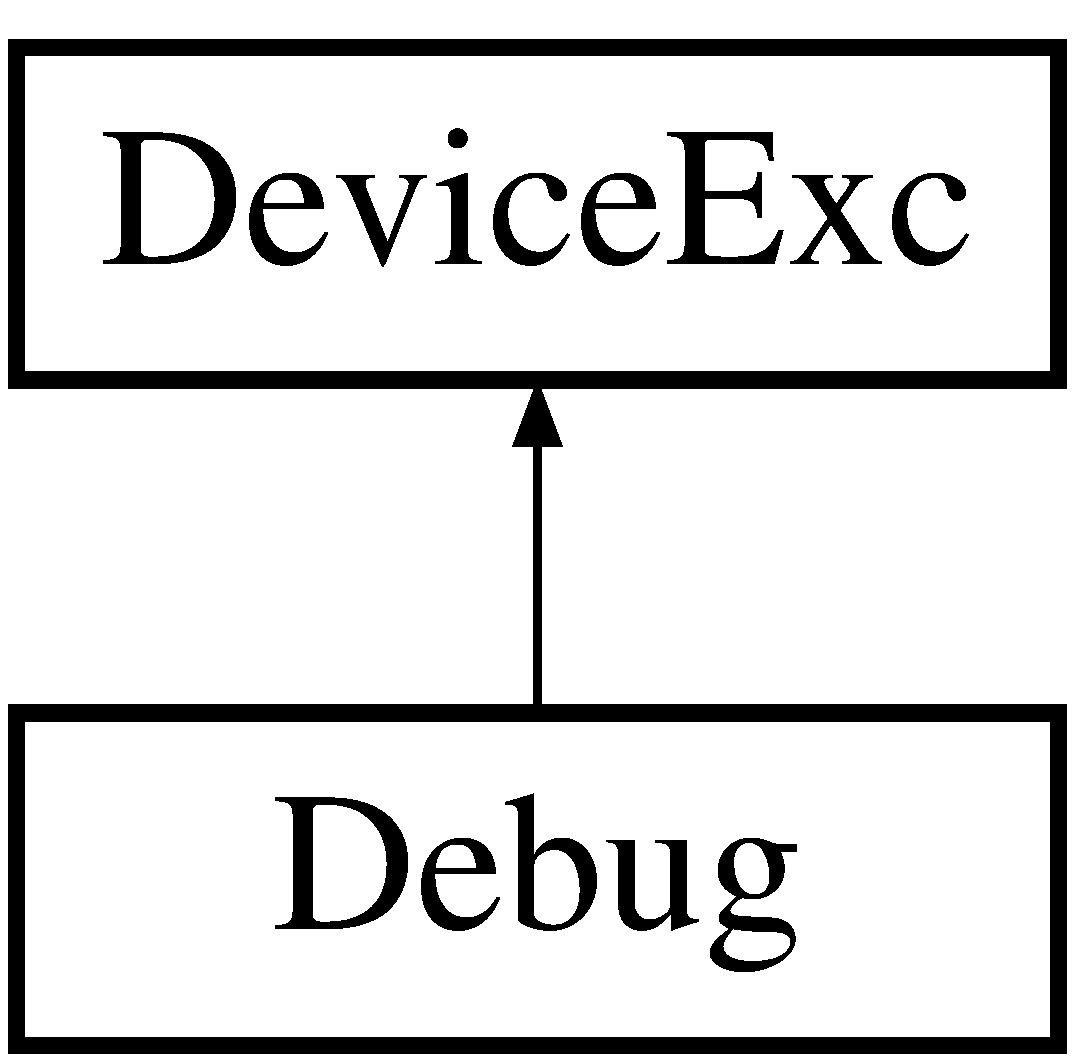
\includegraphics[height=2cm]{classDebug}
\end{center}
\end{figure}
\subsection*{Public Member Functions}
\begin{DoxyCompactItemize}
\item 
\hypertarget{classDebug_a83e8c791e1a70ecaeace305bacab1d04}{
{\bfseries Debug} (\hyperlink{classCPU}{CPU} \&c\_\-, \hyperlink{classMapper}{Mapper} \&m\_\-)}
\label{classDebug_a83e8c791e1a70ecaeace305bacab1d04}

\item 
\hypertarget{classDebug_aa5ea3bb7cd9cadd5274c72b7bbe164fa}{
uint32 {\bfseries packet\_\-pop\_\-word} (char $\ast$$\ast$packet)}
\label{classDebug_aa5ea3bb7cd9cadd5274c72b7bbe164fa}

\item 
\hypertarget{classDebug_ab409b4773599100bf80aeee6f0392291}{
uint8 {\bfseries packet\_\-pop\_\-byte} (char $\ast$$\ast$packet)}
\label{classDebug_ab409b4773599100bf80aeee6f0392291}

\item 
\hypertarget{classDebug_a3a757b15ce3133cd4bc5a503ae2b2439}{
int {\bfseries setup} (uint32 baseaddr, uint32 nwords)}
\label{classDebug_a3a757b15ce3133cd4bc5a503ae2b2439}

\item 
\hypertarget{classDebug_a015e24b9586e31f58fd51b5e0beffdd0}{
int {\bfseries serverloop} (void)}
\label{classDebug_a015e24b9586e31f58fd51b5e0beffdd0}

\item 
\hypertarget{classDebug_ac10c68e808b9198b2577e0d5c29a13ff}{
void {\bfseries exception} (uint16 excCode, int mode, int coprocno)}
\label{classDebug_ac10c68e808b9198b2577e0d5c29a13ff}

\end{DoxyCompactItemize}
\subsection*{Public Attributes}
\begin{DoxyCompactItemize}
\item 
\hypertarget{classDebug_a5c614ecbc3f6d1d782fc531b8fba6be0}{
bool {\bfseries got\_\-interrupt}}
\label{classDebug_a5c614ecbc3f6d1d782fc531b8fba6be0}

\end{DoxyCompactItemize}


The documentation for this class was generated from the following files:\begin{DoxyCompactItemize}
\item 
debug.h\item 
debug.cc\end{DoxyCompactItemize}

\hypertarget{classDECCSRDevice}{
\section{DECCSRDevice Class Reference}
\label{classDECCSRDevice}\index{DECCSRDevice@{DECCSRDevice}}
}
Inheritance diagram for DECCSRDevice:\begin{figure}[H]
\begin{center}
\leavevmode
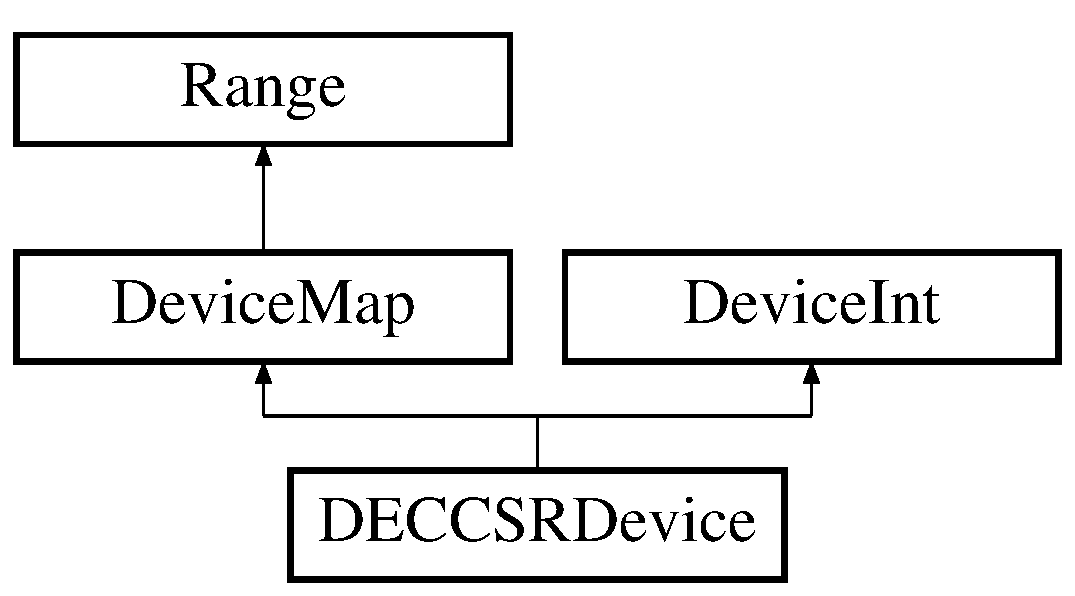
\includegraphics[height=3cm]{classDECCSRDevice}
\end{center}
\end{figure}
\subsection*{Public Member Functions}
\begin{DoxyCompactItemize}
\item 
\hypertarget{classDECCSRDevice_ab00f38e1cd68a11d16e3d5c9ca381af1}{
void {\bfseries assertInt} (uint8 line)}
\label{classDECCSRDevice_ab00f38e1cd68a11d16e3d5c9ca381af1}

\item 
\hypertarget{classDECCSRDevice_a99bb4df90882834bd5c5bcb06457d03d}{
void {\bfseries deassertInt} (uint8 line)}
\label{classDECCSRDevice_a99bb4df90882834bd5c5bcb06457d03d}

\item 
\hypertarget{classDECCSRDevice_a452a8f52b933794f9162ead84814fcd4}{
{\bfseries DECCSRDevice} (uint32 irq\_\-)}
\label{classDECCSRDevice_a452a8f52b933794f9162ead84814fcd4}

\item 
\hypertarget{classDECCSRDevice_a6cc82fe176a5a4e46cf4097ec62f22a0}{
uint32 {\bfseries fetch\_\-word} (uint32 offset, int mode, \hyperlink{classDeviceExc}{DeviceExc} $\ast$client)}
\label{classDECCSRDevice_a6cc82fe176a5a4e46cf4097ec62f22a0}

\item 
\hypertarget{classDECCSRDevice_a9213f37a4ca901a32d22cb61a9cb9d81}{
void {\bfseries store\_\-word} (uint32 offset, uint32 data, \hyperlink{classDeviceExc}{DeviceExc} $\ast$client)}
\label{classDECCSRDevice_a9213f37a4ca901a32d22cb61a9cb9d81}

\item 
\hypertarget{classDECCSRDevice_ada6ce141e4c58bcf6998c00d109c8140}{
const char $\ast$ {\bfseries descriptor\_\-str} () const }
\label{classDECCSRDevice_ada6ce141e4c58bcf6998c00d109c8140}

\end{DoxyCompactItemize}


The documentation for this class was generated from the following files:\begin{DoxyCompactItemize}
\item 
deccsr.h\item 
deccsr.cc\end{DoxyCompactItemize}

\hypertarget{classDECRTCDevice}{
\section{DECRTCDevice Class Reference}
\label{classDECRTCDevice}\index{DECRTCDevice@{DECRTCDevice}}
}
Inheritance diagram for DECRTCDevice:\begin{figure}[H]
\begin{center}
\leavevmode
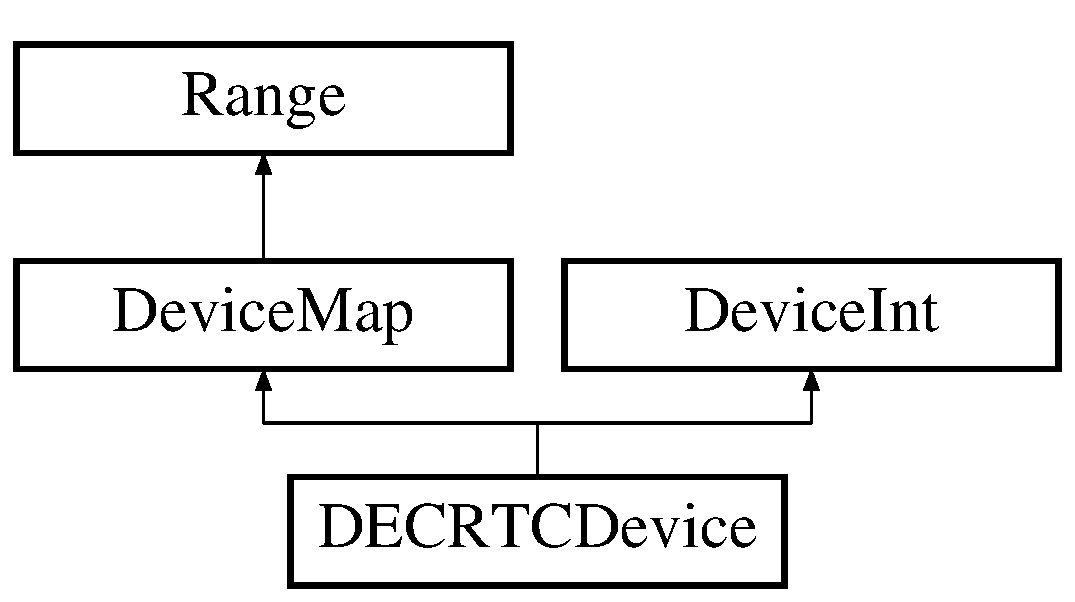
\includegraphics[height=3cm]{classDECRTCDevice}
\end{center}
\end{figure}
\subsection*{Classes}
\begin{DoxyCompactItemize}
\item 
class \hyperlink{classDECRTCDevice_1_1ClockTrigger}{ClockTrigger}
\end{DoxyCompactItemize}
\subsection*{Public Member Functions}
\begin{DoxyCompactItemize}
\item 
\hypertarget{classDECRTCDevice_a1f73f358dc6fb4714cb983696a549a94}{
{\bfseries DECRTCDevice} (\hyperlink{classClock}{Clock} $\ast$\_\-clock, uint32 \_\-irq)}
\label{classDECRTCDevice_a1f73f358dc6fb4714cb983696a549a94}

\item 
\hypertarget{classDECRTCDevice_a89869f71b157a3c6c81a7be897d0e223}{
uint32 {\bfseries fetch\_\-word} (uint32 offset, int mode, \hyperlink{classDeviceExc}{DeviceExc} $\ast$client)}
\label{classDECRTCDevice_a89869f71b157a3c6c81a7be897d0e223}

\item 
\hypertarget{classDECRTCDevice_ad9c476569ab6e229da0ecb9e610f4efb}{
void {\bfseries store\_\-word} (uint32 offset, uint32 data, \hyperlink{classDeviceExc}{DeviceExc} $\ast$client)}
\label{classDECRTCDevice_ad9c476569ab6e229da0ecb9e610f4efb}

\item 
\hypertarget{classDECRTCDevice_a0e319a33e2e91b94f787a4043b796baa}{
const char $\ast$ {\bfseries descriptor\_\-str} () const }
\label{classDECRTCDevice_a0e319a33e2e91b94f787a4043b796baa}

\item 
\hypertarget{classDECRTCDevice_a1e79a0b3fecf8a717dee6454c1f830e0}{
void {\bfseries ready\_\-clock} ()}
\label{classDECRTCDevice_a1e79a0b3fecf8a717dee6454c1f830e0}

\end{DoxyCompactItemize}


The documentation for this class was generated from the following files:\begin{DoxyCompactItemize}
\item 
decrtc.h\item 
decrtc.cc\end{DoxyCompactItemize}

\hypertarget{classDECSerialDevice}{
\section{DECSerialDevice Class Reference}
\label{classDECSerialDevice}\index{DECSerialDevice@{DECSerialDevice}}
}
Inheritance diagram for DECSerialDevice:\begin{figure}[H]
\begin{center}
\leavevmode
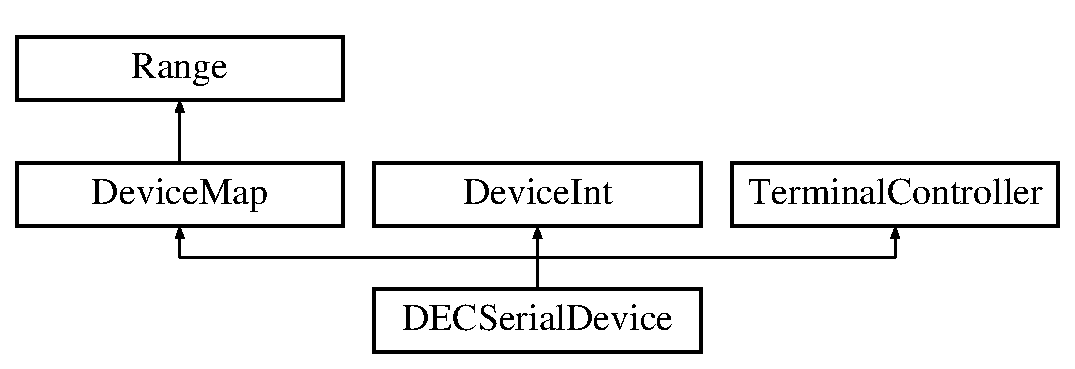
\includegraphics[height=3cm]{classDECSerialDevice}
\end{center}
\end{figure}
\subsection*{Public Member Functions}
\begin{DoxyCompactItemize}
\item 
\hypertarget{classDECSerialDevice_a5352f1903bcbb940a9585d6fdf455e70}{
{\bfseries DECSerialDevice} (\hyperlink{classClock}{Clock} $\ast$clock, uint8 deccsr\_\-irq\_\-)  throw ()}
\label{classDECSerialDevice_a5352f1903bcbb940a9585d6fdf455e70}

\item 
\hypertarget{classDECSerialDevice_a7e7121d53a61efb3b7c6a213b68cbe1f}{
uint32 {\bfseries fetch\_\-word} (uint32 offset, int mode, \hyperlink{classDeviceExc}{DeviceExc} $\ast$client)}
\label{classDECSerialDevice_a7e7121d53a61efb3b7c6a213b68cbe1f}

\item 
\hypertarget{classDECSerialDevice_a703cb7f5757a9076f1074d188291617a}{
void {\bfseries store\_\-word} (uint32 offset, uint32 data, \hyperlink{classDeviceExc}{DeviceExc} $\ast$client)}
\label{classDECSerialDevice_a703cb7f5757a9076f1074d188291617a}

\item 
\hypertarget{classDECSerialDevice_a4bafbd9752125c521627528e8b1c5a2b}{
const char $\ast$ {\bfseries descriptor\_\-str} () const }
\label{classDECSerialDevice_a4bafbd9752125c521627528e8b1c5a2b}

\item 
\hypertarget{classDECSerialDevice_a162892d99421099bcc484975eaa52967}{
virtual void {\bfseries ready\_\-display} (int line)  throw ()}
\label{classDECSerialDevice_a162892d99421099bcc484975eaa52967}

\item 
\hypertarget{classDECSerialDevice_a90c514eea4287882eed3e31f2792964b}{
virtual void {\bfseries unready\_\-display} (int line, char data)  throw (std::bad\_\-alloc)}
\label{classDECSerialDevice_a90c514eea4287882eed3e31f2792964b}

\item 
\hypertarget{classDECSerialDevice_a018c7b26ebc09ce1529549f49a5eb4d4}{
virtual void {\bfseries unready\_\-keyboard} (int line)  throw ()}
\label{classDECSerialDevice_a018c7b26ebc09ce1529549f49a5eb4d4}

\end{DoxyCompactItemize}
\subsection*{Protected Member Functions}
\begin{DoxyCompactItemize}
\item 
\hypertarget{classDECSerialDevice_ac2ab83e7f32d9f70f615eaf3c3121e21}{
virtual void {\bfseries ready\_\-keyboard} (int line)  throw ()}
\label{classDECSerialDevice_ac2ab83e7f32d9f70f615eaf3c3121e21}

\end{DoxyCompactItemize}


The documentation for this class was generated from the following files:\begin{DoxyCompactItemize}
\item 
decserial.h\item 
decserial.cc\end{DoxyCompactItemize}

\hypertarget{classDECStatDevice}{
\section{DECStatDevice Class Reference}
\label{classDECStatDevice}\index{DECStatDevice@{DECStatDevice}}
}
Inheritance diagram for DECStatDevice:\begin{figure}[H]
\begin{center}
\leavevmode
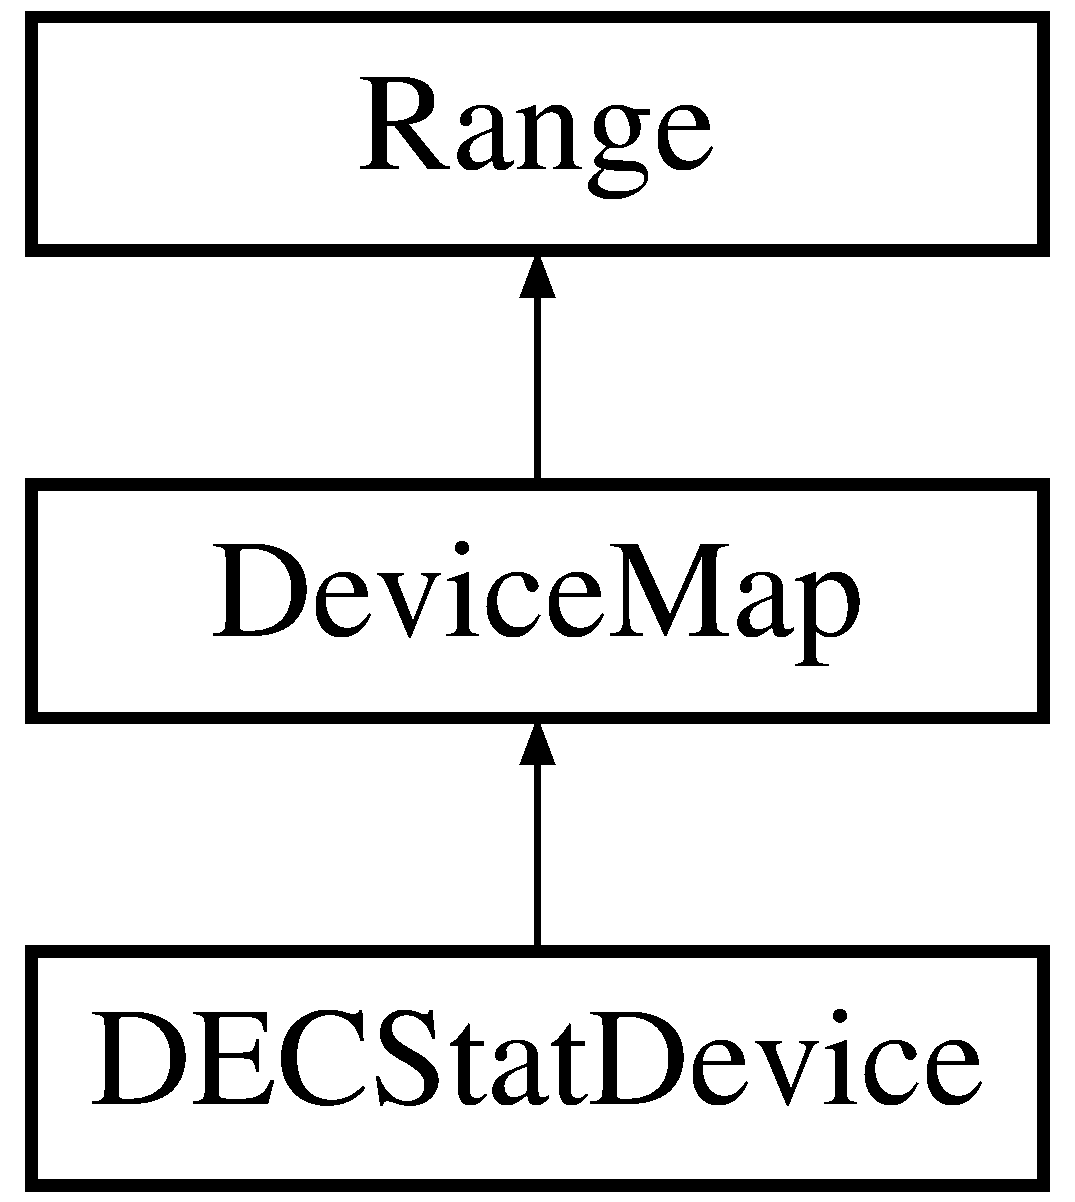
\includegraphics[height=3cm]{classDECStatDevice}
\end{center}
\end{figure}
\subsection*{Public Member Functions}
\begin{DoxyCompactItemize}
\item 
\hypertarget{classDECStatDevice_a15ae2902970cd7ae144572cc169d2e9f}{
uint32 {\bfseries fetch\_\-word} (uint32 offset, int mode, \hyperlink{classDeviceExc}{DeviceExc} $\ast$client)}
\label{classDECStatDevice_a15ae2902970cd7ae144572cc169d2e9f}

\item 
\hypertarget{classDECStatDevice_a5e76b4735aae7b0a5f4475bc461b60a2}{
void {\bfseries store\_\-word} (uint32 offset, uint32 data, \hyperlink{classDeviceExc}{DeviceExc} $\ast$client)}
\label{classDECStatDevice_a5e76b4735aae7b0a5f4475bc461b60a2}

\item 
\hypertarget{classDECStatDevice_a1cdf5669b1c60823487f53628f7c164f}{
const char $\ast$ {\bfseries descriptor\_\-str} () const }
\label{classDECStatDevice_a1cdf5669b1c60823487f53628f7c164f}

\end{DoxyCompactItemize}


The documentation for this class was generated from the following files:\begin{DoxyCompactItemize}
\item 
decstat.h\item 
decstat.cc\end{DoxyCompactItemize}

\hypertarget{classClock_1_1DeferredTasks}{
\section{Clock::DeferredTasks Class Reference}
\label{classClock_1_1DeferredTasks}\index{Clock::DeferredTasks@{Clock::DeferredTasks}}
}
\subsection*{Public Member Functions}
\begin{DoxyCompactItemize}
\item 
\hypertarget{classClock_1_1DeferredTasks_a926f31c0c8b373d47f2ec84d6ecb8456}{
{\bfseries DeferredTasks} (long nanoseconds\_\-left, \hyperlink{classTask}{Task} $\ast$task)  throw ()}
\label{classClock_1_1DeferredTasks_a926f31c0c8b373d47f2ec84d6ecb8456}

\item 
\hypertarget{classClock_1_1DeferredTasks_a9f15b2b4d25c7d5234b1b4bc59bdac44}{
virtual void {\bfseries add\_\-task} (\hyperlink{classTask}{Task} $\ast$task)  throw ()}
\label{classClock_1_1DeferredTasks_a9f15b2b4d25c7d5234b1b4bc59bdac44}

\item 
\hypertarget{classClock_1_1DeferredTasks_a83c3a88b111e960cdcba261f3ab1c969}{
virtual long {\bfseries pass\_\-time} (long nanoseconds)}
\label{classClock_1_1DeferredTasks_a83c3a88b111e960cdcba261f3ab1c969}

\item 
\hypertarget{classClock_1_1DeferredTasks_ab5ebba44377bd518949bd6f93599c0c1}{
virtual long {\bfseries get\_\-nanoseconds\_\-left} ()  throw ()}
\label{classClock_1_1DeferredTasks_ab5ebba44377bd518949bd6f93599c0c1}

\end{DoxyCompactItemize}
\subsection*{Protected Attributes}
\begin{DoxyCompactItemize}
\item 
\hypertarget{classClock_1_1DeferredTasks_a6db5d7ddd158bef346c20a9792b57f3f}{
long {\bfseries nanoseconds\_\-left}}
\label{classClock_1_1DeferredTasks_a6db5d7ddd158bef346c20a9792b57f3f}

\item 
\hypertarget{classClock_1_1DeferredTasks_a17581b0d310a9d7ca041d50698edaeff}{
std::list$<$ \hyperlink{classTask}{Task} $\ast$ $>$ {\bfseries tasks}}
\label{classClock_1_1DeferredTasks_a17581b0d310a9d7ca041d50698edaeff}

\end{DoxyCompactItemize}


The documentation for this class was generated from the following files:\begin{DoxyCompactItemize}
\item 
clock.h\item 
clock.cc\end{DoxyCompactItemize}

\hypertarget{classDeviceExc}{
\section{DeviceExc Class Reference}
\label{classDeviceExc}\index{DeviceExc@{DeviceExc}}
}
Inheritance diagram for DeviceExc:\begin{figure}[H]
\begin{center}
\leavevmode
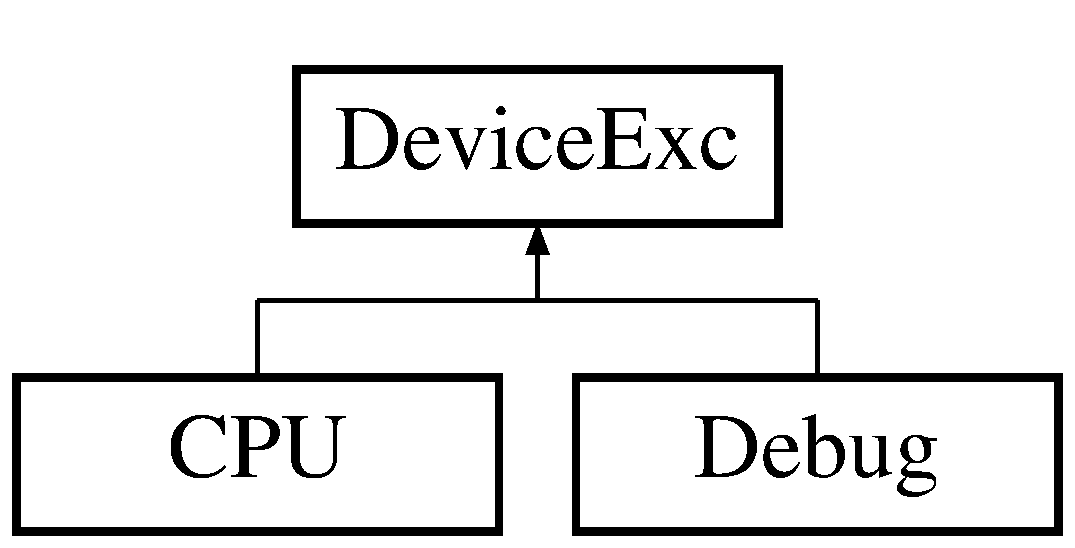
\includegraphics[height=2cm]{classDeviceExc}
\end{center}
\end{figure}
\subsection*{Public Member Functions}
\begin{DoxyCompactItemize}
\item 
\hypertarget{classDeviceExc_adfa40efde878b6499d3ffc66b4fa7166}{
virtual void {\bfseries exception} (uint16 excCode, int mode=ANY, int coprocno=-\/1)=0}
\label{classDeviceExc_adfa40efde878b6499d3ffc66b4fa7166}

\end{DoxyCompactItemize}
\subsection*{Public Attributes}
\begin{DoxyCompactItemize}
\item 
\hypertarget{classDeviceExc_affa8f27155e9b97d0f2d76383a29489f}{
bool {\bfseries exception\_\-pending}}
\label{classDeviceExc_affa8f27155e9b97d0f2d76383a29489f}

\end{DoxyCompactItemize}


The documentation for this class was generated from the following file:\begin{DoxyCompactItemize}
\item 
deviceexc.h\end{DoxyCompactItemize}

\hypertarget{classDeviceInt}{
\section{DeviceInt Class Reference}
\label{classDeviceInt}\index{DeviceInt@{DeviceInt}}
}
Inheritance diagram for DeviceInt:\begin{figure}[H]
\begin{center}
\leavevmode
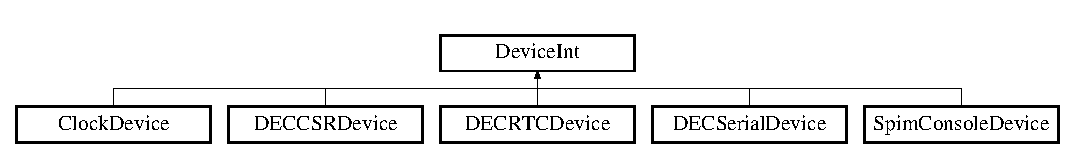
\includegraphics[height=1.68421cm]{classDeviceInt}
\end{center}
\end{figure}
\subsection*{Static Public Member Functions}
\begin{DoxyCompactItemize}
\item 
\hypertarget{classDeviceInt_a7b51658efadb002993df8b4475ce29eb}{
static char $\ast$ {\bfseries strlineno} (uint32 line)}
\label{classDeviceInt_a7b51658efadb002993df8b4475ce29eb}

\item 
\hypertarget{classDeviceInt_a5a1c12ade91f0bf325a26988555f9989}{
static uint32 {\bfseries num2irq} (uint32 num)  throw ()}
\label{classDeviceInt_a5a1c12ade91f0bf325a26988555f9989}

\end{DoxyCompactItemize}
\subsection*{Protected Member Functions}
\begin{DoxyCompactItemize}
\item 
\hypertarget{classDeviceInt_a2b7e17c5314630680c3a09a9e706f870}{
void {\bfseries assertInt} (uint32 line)}
\label{classDeviceInt_a2b7e17c5314630680c3a09a9e706f870}

\item 
\hypertarget{classDeviceInt_ad7387f17b6dfa6acf90e857a7e33aa01}{
void {\bfseries deassertInt} (uint32 line)}
\label{classDeviceInt_ad7387f17b6dfa6acf90e857a7e33aa01}

\item 
\hypertarget{classDeviceInt_a8e93853ae77b6a63a140ed498d9fc8b8}{
virtual const char $\ast$ {\bfseries descriptor\_\-str} (void) const =0}
\label{classDeviceInt_a8e93853ae77b6a63a140ed498d9fc8b8}

\end{DoxyCompactItemize}
\subsection*{Friends}
\begin{DoxyCompactItemize}
\item 
\hypertarget{classDeviceInt_aa29a2d47613fcc0b21d2babf280a2c7f}{
class \hyperlink{classDeviceInt_aa29a2d47613fcc0b21d2babf280a2c7f}{IntCtrl}}
\label{classDeviceInt_aa29a2d47613fcc0b21d2babf280a2c7f}

\end{DoxyCompactItemize}


The documentation for this class was generated from the following files:\begin{DoxyCompactItemize}
\item 
deviceint.h\item 
deviceint.cc\end{DoxyCompactItemize}

\hypertarget{classDeviceMap}{
\section{DeviceMap Class Reference}
\label{classDeviceMap}\index{DeviceMap@{DeviceMap}}
}
Inheritance diagram for DeviceMap:\begin{figure}[H]
\begin{center}
\leavevmode
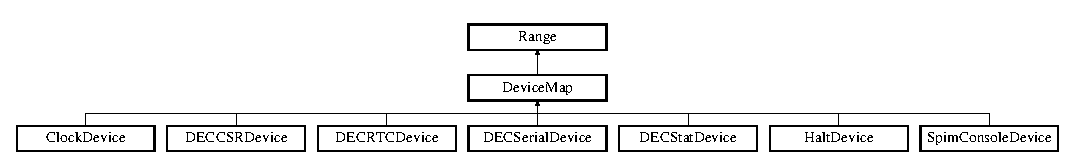
\includegraphics[height=1.80451cm]{classDeviceMap}
\end{center}
\end{figure}
\subsection*{Public Member Functions}
\begin{DoxyCompactItemize}
\item 
\hypertarget{classDeviceMap_aa3051a16728bec8261d031e62edb4fca}{
virtual uint32 {\bfseries fetch\_\-word} (uint32 offset, int mode, \hyperlink{classDeviceExc}{DeviceExc} $\ast$client)=0}
\label{classDeviceMap_aa3051a16728bec8261d031e62edb4fca}

\item 
\hypertarget{classDeviceMap_ac71109d80a98cd1617292f451eed8d36}{
virtual uint16 {\bfseries fetch\_\-halfword} (uint32 offset, \hyperlink{classDeviceExc}{DeviceExc} $\ast$client)}
\label{classDeviceMap_ac71109d80a98cd1617292f451eed8d36}

\item 
\hypertarget{classDeviceMap_a01a27bd6f0a6fbe029609c3a72abde70}{
virtual uint8 {\bfseries fetch\_\-byte} (uint32 offset, \hyperlink{classDeviceExc}{DeviceExc} $\ast$client)}
\label{classDeviceMap_a01a27bd6f0a6fbe029609c3a72abde70}

\item 
\hypertarget{classDeviceMap_a35fca28f44abbd13f9db1e32651b1a10}{
virtual void {\bfseries store\_\-word} (uint32 offset, uint32 data, \hyperlink{classDeviceExc}{DeviceExc} $\ast$client)=0}
\label{classDeviceMap_a35fca28f44abbd13f9db1e32651b1a10}

\item 
\hypertarget{classDeviceMap_a24ff12255b493fc390ffee1241283f8c}{
virtual void {\bfseries store\_\-halfword} (uint32 offset, uint16 data, \hyperlink{classDeviceExc}{DeviceExc} $\ast$client)}
\label{classDeviceMap_a24ff12255b493fc390ffee1241283f8c}

\item 
\hypertarget{classDeviceMap_a2f0ec5a2d3ed8191645d99f3ab555dce}{
virtual void {\bfseries store\_\-byte} (uint32 offset, uint8 data, \hyperlink{classDeviceExc}{DeviceExc} $\ast$client)}
\label{classDeviceMap_a2f0ec5a2d3ed8191645d99f3ab555dce}

\item 
\hypertarget{classDeviceMap_aa4465202ceece719ceb26d24c6a5f454}{
virtual bool {\bfseries canRead} (uint32 offset)  throw ()}
\label{classDeviceMap_aa4465202ceece719ceb26d24c6a5f454}

\item 
\hypertarget{classDeviceMap_a2257514fbcd9acc310cfba5f12574451}{
virtual bool {\bfseries canWrite} (uint32 offset)  throw ()}
\label{classDeviceMap_a2257514fbcd9acc310cfba5f12574451}

\end{DoxyCompactItemize}
\subsection*{Protected Member Functions}
\begin{DoxyCompactItemize}
\item 
\hypertarget{classDeviceMap_ae385e56171b31f2ee27d96e9623d64af}{
{\bfseries DeviceMap} (uint32 \_\-extent)  throw ()}
\label{classDeviceMap_ae385e56171b31f2ee27d96e9623d64af}

\end{DoxyCompactItemize}


The documentation for this class was generated from the following files:\begin{DoxyCompactItemize}
\item 
devicemap.h\item 
devicemap.cc\end{DoxyCompactItemize}

\hypertarget{classDisassembler}{
\section{Disassembler Class Reference}
\label{classDisassembler}\index{Disassembler@{Disassembler}}
}
\subsection*{Public Member Functions}
\begin{DoxyCompactItemize}
\item 
\hypertarget{classDisassembler_adae55d4f2ea0e1e676109cb29100f396}{
{\bfseries Disassembler} (bool host\_\-is\_\-bigendian, FILE $\ast$stream)}
\label{classDisassembler_adae55d4f2ea0e1e676109cb29100f396}

\item 
\hypertarget{classDisassembler_aa45c52f0704884adb330b4c1c052d5b7}{
void {\bfseries disassemble} (uint32 pc, uint32 instr)}
\label{classDisassembler_aa45c52f0704884adb330b4c1c052d5b7}

\end{DoxyCompactItemize}


The documentation for this class was generated from the following files:\begin{DoxyCompactItemize}
\item 
stub-\/dis.h\item 
stub-\/dis.cc\end{DoxyCompactItemize}

\hypertarget{classTerminalController_1_1DisplayDelay}{
\section{TerminalController::DisplayDelay Class Reference}
\label{classTerminalController_1_1DisplayDelay}\index{TerminalController::DisplayDelay@{TerminalController::DisplayDelay}}
}
Inheritance diagram for TerminalController::DisplayDelay:\begin{figure}[H]
\begin{center}
\leavevmode
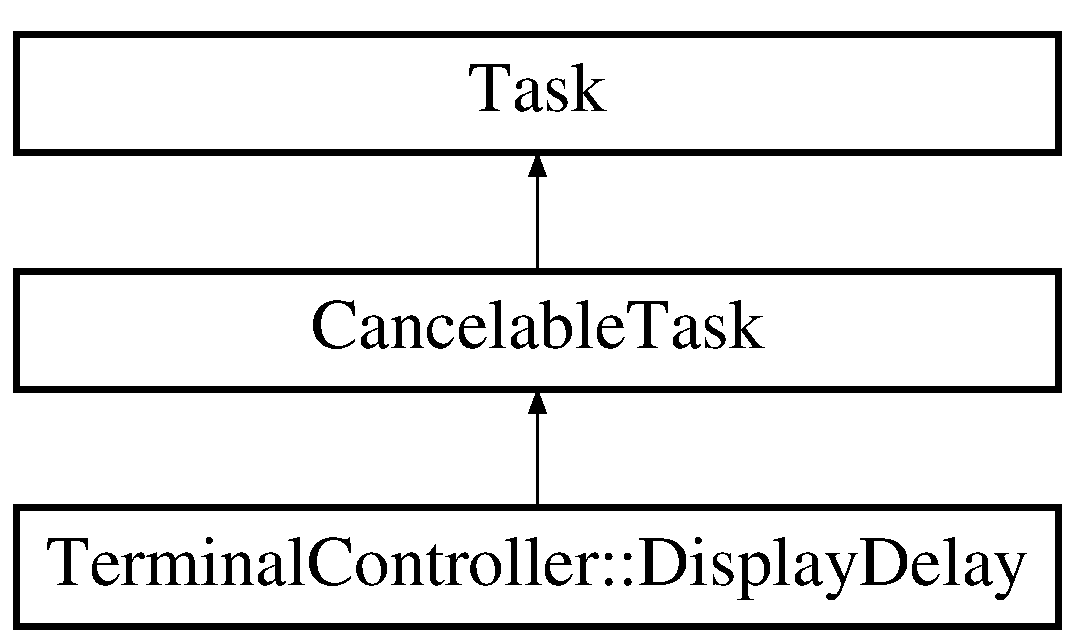
\includegraphics[height=3cm]{classTerminalController_1_1DisplayDelay}
\end{center}
\end{figure}
\subsection*{Public Member Functions}
\begin{DoxyCompactItemize}
\item 
\hypertarget{classTerminalController_1_1DisplayDelay_a1b2a24dac56b2f23c17e8dd2ef1e3d75}{
{\bfseries DisplayDelay} (\hyperlink{classTerminalController}{TerminalController} $\ast$controller, int line)  throw ()}
\label{classTerminalController_1_1DisplayDelay_a1b2a24dac56b2f23c17e8dd2ef1e3d75}

\end{DoxyCompactItemize}
\subsection*{Protected Member Functions}
\begin{DoxyCompactItemize}
\item 
\hypertarget{classTerminalController_1_1DisplayDelay_abe0f542df1df0437944ece955879da69}{
virtual void {\bfseries real\_\-task} ()}
\label{classTerminalController_1_1DisplayDelay_abe0f542df1df0437944ece955879da69}

\end{DoxyCompactItemize}
\subsection*{Protected Attributes}
\begin{DoxyCompactItemize}
\item 
\hypertarget{classTerminalController_1_1DisplayDelay_aa03cf51bb4fdcaad09b8ee962f9e8c2e}{
\hyperlink{classTerminalController}{TerminalController} $\ast$ {\bfseries controller}}
\label{classTerminalController_1_1DisplayDelay_aa03cf51bb4fdcaad09b8ee962f9e8c2e}

\item 
\hypertarget{classTerminalController_1_1DisplayDelay_a4bf95671db0f400ac76617427e5fa0e9}{
int {\bfseries line}}
\label{classTerminalController_1_1DisplayDelay_a4bf95671db0f400ac76617427e5fa0e9}

\end{DoxyCompactItemize}


The documentation for this class was generated from the following files:\begin{DoxyCompactItemize}
\item 
terminalcontroller.h\item 
terminalcontroller.cc\end{DoxyCompactItemize}

\hypertarget{classPlog_1_1End}{
\section{Plog::End Class Reference}
\label{classPlog_1_1End}\index{Plog::End@{Plog::End}}
}


The documentation for this class was generated from the following file:\begin{DoxyCompactItemize}
\item 
prophetlog.h\end{DoxyCompactItemize}

\hypertarget{classEndianSelfTester}{
\section{EndianSelfTester Class Reference}
\label{classEndianSelfTester}\index{EndianSelfTester@{EndianSelfTester}}
}
\subsection*{Public Member Functions}
\begin{DoxyCompactItemize}
\item 
\hypertarget{classEndianSelfTester_a1ac98cdbcbfaa82f42a9a283b0b81585}{
bool {\bfseries host\_\-is\_\-big\_\-endian} () const }
\label{classEndianSelfTester_a1ac98cdbcbfaa82f42a9a283b0b81585}

\end{DoxyCompactItemize}


The documentation for this class was generated from the following file:\begin{DoxyCompactItemize}
\item 
endiantest.h\end{DoxyCompactItemize}

\hypertarget{structexcPriority}{
\section{excPriority Struct Reference}
\label{structexcPriority}\index{excPriority@{excPriority}}
}
\subsection*{Public Attributes}
\begin{DoxyCompactItemize}
\item 
\hypertarget{structexcPriority_a39a726a654eba6f653e0ade494218f40}{
int {\bfseries priority}}
\label{structexcPriority_a39a726a654eba6f653e0ade494218f40}

\item 
\hypertarget{structexcPriority_a056c56096bbf838f85991bd1b069072e}{
int {\bfseries excCode}}
\label{structexcPriority_a056c56096bbf838f85991bd1b069072e}

\item 
\hypertarget{structexcPriority_a3cf74f18cde52f3f849ae26897141de4}{
int {\bfseries mode}}
\label{structexcPriority_a3cf74f18cde52f3f849ae26897141de4}

\end{DoxyCompactItemize}


The documentation for this struct was generated from the following file:\begin{DoxyCompactItemize}
\item 
cpu.h\end{DoxyCompactItemize}

\hypertarget{classPlog_1_1FileRecorder}{
\section{Plog::FileRecorder Class Reference}
\label{classPlog_1_1FileRecorder}\index{Plog::FileRecorder@{Plog::FileRecorder}}
}
Inheritance diagram for Plog::FileRecorder:\begin{figure}[H]
\begin{center}
\leavevmode
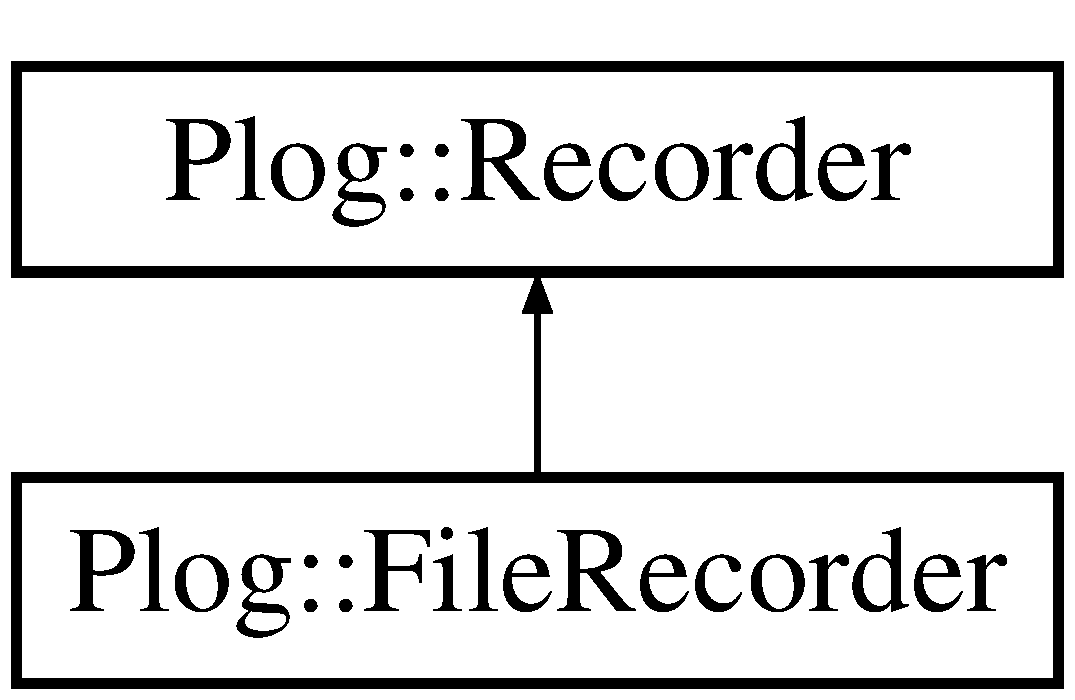
\includegraphics[height=2cm]{classPlog_1_1FileRecorder}
\end{center}
\end{figure}
\subsection*{Public Member Functions}
\begin{DoxyCompactItemize}
\item 
\hypertarget{classPlog_1_1FileRecorder_af397f154039c536cd86aeeae729009d2}{
{\bfseries FileRecorder} (const char $\ast$file)}
\label{classPlog_1_1FileRecorder_af397f154039c536cd86aeeae729009d2}

\item 
\hypertarget{classPlog_1_1FileRecorder_a39a37f25e913858b9b4bcfefcabb114f}{
virtual void {\bfseries RecordMessage} (Plog::PLOG\_\-LEVEL level, const std::string \&message)}
\label{classPlog_1_1FileRecorder_a39a37f25e913858b9b4bcfefcabb114f}

\end{DoxyCompactItemize}


The documentation for this class was generated from the following file:\begin{DoxyCompactItemize}
\item 
prophetlog.cc\end{DoxyCompactItemize}

\hypertarget{classFPU}{
\section{FPU Class Reference}
\label{classFPU}\index{FPU@{FPU}}
}
\subsection*{Public Member Functions}
\begin{DoxyCompactItemize}
\item 
\hypertarget{classFPU_a358d735dc50060c3eb2d416e8d6d8ff7}{
void {\bfseries interpret\_\-float\_\-value} (uint32, float \&)}
\label{classFPU_a358d735dc50060c3eb2d416e8d6d8ff7}

\item 
\hypertarget{classFPU_a4e2113932d665c4e45d7e88c63ddde36}{
void {\bfseries interpret\_\-double\_\-value} (uint64, double \&d)}
\label{classFPU_a4e2113932d665c4e45d7e88c63ddde36}

\item 
\hypertarget{classFPU_a0d9e4de6caf810ebc70e5494f154c99b}{
uint32 {\bfseries uninterpret\_\-float\_\-value} (float f)}
\label{classFPU_a0d9e4de6caf810ebc70e5494f154c99b}

\item 
\hypertarget{classFPU_a5318f58aa92a78c76b309f4a7f5c48a6}{
uint64 {\bfseries uninterpret\_\-double\_\-value} (double d)}
\label{classFPU_a5318f58aa92a78c76b309f4a7f5c48a6}

\item 
\hypertarget{classFPU_aef477ba456ce9008c3ae7e09072b02ed}{
void {\bfseries mfc1\_\-emulate} (uint32 instr, uint32 pc)}
\label{classFPU_aef477ba456ce9008c3ae7e09072b02ed}

\item 
\hypertarget{classFPU_ad0c56d545fee64d72cccdec95fad89af}{
void {\bfseries mtc1\_\-emulate} (uint32 instr, uint32 pc)}
\label{classFPU_ad0c56d545fee64d72cccdec95fad89af}

\item 
\hypertarget{classFPU_a54474473a52874ff909713e0091c3112}{
void {\bfseries adds\_\-emulate} (uint32 instr, uint32 pc)}
\label{classFPU_a54474473a52874ff909713e0091c3112}

\item 
\hypertarget{classFPU_a973f43b95694b7b27c8db702350a1ce6}{
void {\bfseries addd\_\-emulate} (uint32 instr, uint32 pc)}
\label{classFPU_a973f43b95694b7b27c8db702350a1ce6}

\item 
\hypertarget{classFPU_a8f755a58d7463db6324e093fc9f83fa7}{
void {\bfseries subs\_\-emulate} (uint32 instr, uint32 pc)}
\label{classFPU_a8f755a58d7463db6324e093fc9f83fa7}

\item 
\hypertarget{classFPU_a7ee6226cb58ef1fdc21157d9fe7036dc}{
void {\bfseries subd\_\-emulate} (uint32 instr, uint32 pc)}
\label{classFPU_a7ee6226cb58ef1fdc21157d9fe7036dc}

\item 
\hypertarget{classFPU_ad4ae687cb716f811d601cace20f883a6}{
void {\bfseries muls\_\-emulate} (uint32 instr, uint32 pc)}
\label{classFPU_ad4ae687cb716f811d601cace20f883a6}

\item 
\hypertarget{classFPU_a7850950f4e2a725d9dc6ea3c36af5786}{
void {\bfseries muld\_\-emulate} (uint32 instr, uint32 pc)}
\label{classFPU_a7850950f4e2a725d9dc6ea3c36af5786}

\item 
\hypertarget{classFPU_a4ba3a1b7552964876d23beb60162a390}{
void {\bfseries divs\_\-emulate} (uint32 instr, uint32 pc)}
\label{classFPU_a4ba3a1b7552964876d23beb60162a390}

\item 
\hypertarget{classFPU_a95f4b075be936d582b2ec856c520d8f7}{
void {\bfseries divd\_\-emulate} (uint32 instr, uint32 pc)}
\label{classFPU_a95f4b075be936d582b2ec856c520d8f7}

\item 
\hypertarget{classFPU_aa9bd06dbe14b181296977d830f98dce7}{
void {\bfseries abss\_\-emulate} (uint32 instr, uint32 pc)}
\label{classFPU_aa9bd06dbe14b181296977d830f98dce7}

\item 
\hypertarget{classFPU_a444a0fbf10bf86a785590f67c6e9eba3}{
void {\bfseries absd\_\-emulate} (uint32 instr, uint32 pc)}
\label{classFPU_a444a0fbf10bf86a785590f67c6e9eba3}

\item 
\hypertarget{classFPU_a1fa93a22a15dd20327642f3a371ebde7}{
void {\bfseries movs\_\-emulate} (uint32 instr, uint32 pc)}
\label{classFPU_a1fa93a22a15dd20327642f3a371ebde7}

\item 
\hypertarget{classFPU_a2ac46d52ed795327e1a7d41e8ae2f104}{
void {\bfseries movd\_\-emulate} (uint32 instr, uint32 pc)}
\label{classFPU_a2ac46d52ed795327e1a7d41e8ae2f104}

\item 
\hypertarget{classFPU_a6d4242b059ac00a92786b5b02b1f68ad}{
void {\bfseries negs\_\-emulate} (uint32 instr, uint32 pc)}
\label{classFPU_a6d4242b059ac00a92786b5b02b1f68ad}

\item 
\hypertarget{classFPU_a535c953956b80d1e1e19d486b581ae40}{
void {\bfseries negd\_\-emulate} (uint32 instr, uint32 pc)}
\label{classFPU_a535c953956b80d1e1e19d486b581ae40}

\item 
\hypertarget{classFPU_a700c7159f311ed08d8bee659181852a0}{
void {\bfseries cvtsd\_\-emulate} (uint32 instr, uint32 pc)}
\label{classFPU_a700c7159f311ed08d8bee659181852a0}

\item 
\hypertarget{classFPU_a8a077ccd5ff9bd9236d89fd643fb1d85}{
void {\bfseries cvtsw\_\-emulate} (uint32 instr, uint32 pc)}
\label{classFPU_a8a077ccd5ff9bd9236d89fd643fb1d85}

\item 
\hypertarget{classFPU_a4686e932ae0345e75be19be78f882e78}{
void {\bfseries cvtds\_\-emulate} (uint32 instr, uint32 pc)}
\label{classFPU_a4686e932ae0345e75be19be78f882e78}

\item 
\hypertarget{classFPU_a2ee26225f9d1627129ed20b308eb7779}{
void {\bfseries cvtdw\_\-emulate} (uint32 instr, uint32 pc)}
\label{classFPU_a2ee26225f9d1627129ed20b308eb7779}

\item 
\hypertarget{classFPU_af0acd850a4a015b22d9122f21aab0694}{
void {\bfseries cvtws\_\-emulate} (uint32 instr, uint32 pc)}
\label{classFPU_af0acd850a4a015b22d9122f21aab0694}

\item 
\hypertarget{classFPU_aa24cb85a5d3113cf33956954acf23c5d}{
void {\bfseries cvtwd\_\-emulate} (uint32 instr, uint32 pc)}
\label{classFPU_aa24cb85a5d3113cf33956954acf23c5d}

\item 
\hypertarget{classFPU_a755d779270698baf5183494a73311601}{
void {\bfseries csfs\_\-emulate} (uint32 instr, uint32 pc)}
\label{classFPU_a755d779270698baf5183494a73311601}

\item 
\hypertarget{classFPU_a0ac2cf827201ac46cc5c6edbff77f83b}{
void {\bfseries csfd\_\-emulate} (uint32 instr, uint32 pc)}
\label{classFPU_a0ac2cf827201ac46cc5c6edbff77f83b}

\item 
\hypertarget{classFPU_a9ce1fb5bb15b767a978461e19f7a8794}{
void {\bfseries cseqs\_\-emulate} (uint32 instr, uint32 pc)}
\label{classFPU_a9ce1fb5bb15b767a978461e19f7a8794}

\item 
\hypertarget{classFPU_a57085dc91c1d644a9dd1dfa7c6235f58}{
void {\bfseries cseqd\_\-emulate} (uint32 instr, uint32 pc)}
\label{classFPU_a57085dc91c1d644a9dd1dfa7c6235f58}

\item 
\hypertarget{classFPU_a474ea0a72b3aa046deefa32fb4c7e8b2}{
void {\bfseries clts\_\-emulate} (uint32 instr, uint32 pc)}
\label{classFPU_a474ea0a72b3aa046deefa32fb4c7e8b2}

\item 
\hypertarget{classFPU_a49b0cc0e170f59dbfcbbc46eb96fa7cd}{
void {\bfseries cltd\_\-emulate} (uint32 instr, uint32 pc)}
\label{classFPU_a49b0cc0e170f59dbfcbbc46eb96fa7cd}

\item 
\hypertarget{classFPU_af7d7d86382989aefef81d8f4a6f8bcd4}{
void {\bfseries cles\_\-emulate} (uint32 instr, uint32 pc)}
\label{classFPU_af7d7d86382989aefef81d8f4a6f8bcd4}

\item 
\hypertarget{classFPU_a6764d43d5047b524de49904bf2e03d38}{
void {\bfseries cled\_\-emulate} (uint32 instr, uint32 pc)}
\label{classFPU_a6764d43d5047b524de49904bf2e03d38}

\item 
\hypertarget{classFPU_ad88746f20edf49cd5b23c1ed0fa2b2b9}{
void {\bfseries bc1f\_\-emulate} (uint32 instr, uint32 pc)}
\label{classFPU_ad88746f20edf49cd5b23c1ed0fa2b2b9}

\item 
\hypertarget{classFPU_a1f206e5e99c26c62d47e66d298b8f7b8}{
void {\bfseries bc1t\_\-emulate} (uint32 instr, uint32 pc)}
\label{classFPU_a1f206e5e99c26c62d47e66d298b8f7b8}

\item 
\hypertarget{classFPU_a7772a53202d001dc8ea724778b10684f}{
void {\bfseries cpone\_\-emulate} (uint32 instr, uint32 pc)}
\label{classFPU_a7772a53202d001dc8ea724778b10684f}

\item 
\hypertarget{classFPU_a1cbfbf811bb78caad1d27fb10f701782}{
{\bfseries FPU} (SpeculativeCPU $\ast$m, \hyperlink{classIntCtrl}{IntCtrl} $\ast$i)}
\label{classFPU_a1cbfbf811bb78caad1d27fb10f701782}

\item 
\hypertarget{classFPU_a88f9eec5026c8cbb0221fbd0491d3140}{
void {\bfseries Clear\_\-condition} (uint32 \&)}
\label{classFPU_a88f9eec5026c8cbb0221fbd0491d3140}

\item 
\hypertarget{classFPU_a5520a13dac0d050832a245f43f6d5a38}{
void {\bfseries Set\_\-condition} (uint32 \&)}
\label{classFPU_a5520a13dac0d050832a245f43f6d5a38}

\item 
\hypertarget{classFPU_a279cdfd9bfd4d95200ad050a796d8c65}{
void {\bfseries reset} ()}
\label{classFPU_a279cdfd9bfd4d95200ad050a796d8c65}

\item 
\hypertarget{classFPU_aecbf73903f26ca2ebbfaacefa154bb71}{
bool {\bfseries Float\_\-is\_\-NAN} (uint32)}
\label{classFPU_aecbf73903f26ca2ebbfaacefa154bb71}

\item 
\hypertarget{classFPU_ac2c3bf00c3a2c1c1fe81f1dd44b446ac}{
bool {\bfseries Double\_\-is\_\-NAN} (uint64)}
\label{classFPU_ac2c3bf00c3a2c1c1fe81f1dd44b446ac}

\item 
\hypertarget{classFPU_a33b65557a53a4e30657bc9cbb6e43a63}{
bool {\bfseries Fpcondition} (uint32)}
\label{classFPU_a33b65557a53a4e30657bc9cbb6e43a63}

\item 
\hypertarget{classFPU_aebbaa139c9609776428483b9b44f3da9}{
uint16 {\bfseries ft} (const uint32 instr) const }
\label{classFPU_aebbaa139c9609776428483b9b44f3da9}

\end{DoxyCompactItemize}
\subsection*{Public Attributes}
\begin{DoxyCompactItemize}
\item 
\hypertarget{classFPU_a55769238d4733e7f9ac6c2b49d467e62}{
uint32 {\bfseries freg} \mbox{[}32\mbox{]}}
\label{classFPU_a55769238d4733e7f9ac6c2b49d467e62}

\item 
\hypertarget{classFPU_a2cd01292739db9bfd89ea10fc9d6ed2c}{
SpeculativeCPU $\ast$ {\bfseries speculativecpu}}
\label{classFPU_a2cd01292739db9bfd89ea10fc9d6ed2c}

\item 
\hypertarget{classFPU_aea75f0e2d3c4914c567d87d9f7a63a39}{
\hyperlink{classIntCtrl}{IntCtrl} $\ast$ {\bfseries intc}}
\label{classFPU_aea75f0e2d3c4914c567d87d9f7a63a39}

\end{DoxyCompactItemize}


The documentation for this class was generated from the following files:\begin{DoxyCompactItemize}
\item 
prophetfpu.h\item 
prophetfpu.cc\end{DoxyCompactItemize}

\hypertarget{classHaltDevice}{
\section{HaltDevice Class Reference}
\label{classHaltDevice}\index{HaltDevice@{HaltDevice}}
}
Inheritance diagram for HaltDevice:\begin{figure}[H]
\begin{center}
\leavevmode
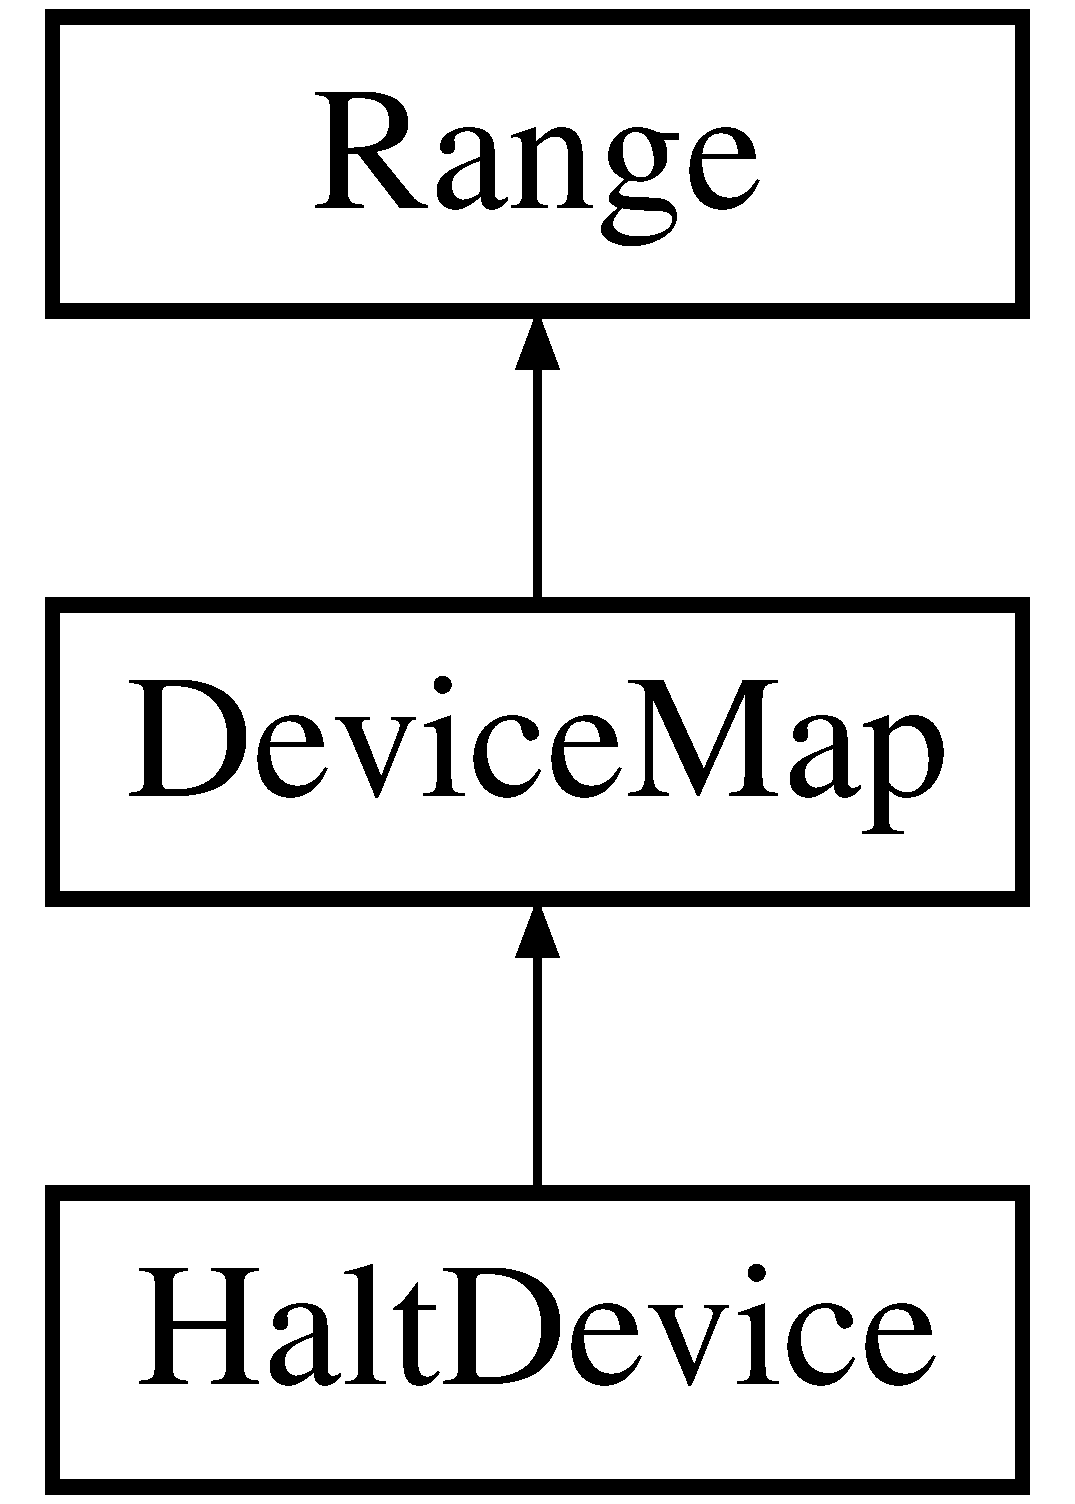
\includegraphics[height=3cm]{classHaltDevice}
\end{center}
\end{figure}
\subsection*{Public Member Functions}
\begin{DoxyCompactItemize}
\item 
\hypertarget{classHaltDevice_ab4948d58e6b7efd5b978ac2069c935d1}{
{\bfseries HaltDevice} (\hyperlink{classvmips}{vmips} $\ast$machine)  throw ()}
\label{classHaltDevice_ab4948d58e6b7efd5b978ac2069c935d1}

\item 
\hypertarget{classHaltDevice_a59cd92570eb9689b67656e6e92ea3457}{
virtual uint32 {\bfseries fetch\_\-word} (uint32 offset, int mode, \hyperlink{classDeviceExc}{DeviceExc} $\ast$client)}
\label{classHaltDevice_a59cd92570eb9689b67656e6e92ea3457}

\item 
\hypertarget{classHaltDevice_a4f13e32c5f0734bae65fe9c62b402e9f}{
virtual void {\bfseries store\_\-word} (uint32 offset, uint32 data, \hyperlink{classDeviceExc}{DeviceExc} $\ast$client)}
\label{classHaltDevice_a4f13e32c5f0734bae65fe9c62b402e9f}

\item 
\hypertarget{classHaltDevice_a6ff3fc3006786f97b201c3481084ca90}{
char $\ast$ {\bfseries descriptor\_\-str} ()}
\label{classHaltDevice_a6ff3fc3006786f97b201c3481084ca90}

\end{DoxyCompactItemize}
\subsection*{Protected Attributes}
\begin{DoxyCompactItemize}
\item 
\hypertarget{classHaltDevice_a025cb05a489514495a72b98123c62e87}{
\hyperlink{classvmips}{vmips} $\ast$ {\bfseries machine}}
\label{classHaltDevice_a025cb05a489514495a72b98123c62e87}

\end{DoxyCompactItemize}


The documentation for this class was generated from the following files:\begin{DoxyCompactItemize}
\item 
haltdev.h\item 
haltdev.cc\end{DoxyCompactItemize}

\hypertarget{classIntCtrl}{
\section{IntCtrl Class Reference}
\label{classIntCtrl}\index{IntCtrl@{IntCtrl}}
}
\subsection*{Public Member Functions}
\begin{DoxyCompactItemize}
\item 
\hypertarget{classIntCtrl_a62f4eae5fbfd7c96852003b02f95c69c}{
virtual uint32 {\bfseries calculateIP} ()  throw ()}
\label{classIntCtrl_a62f4eae5fbfd7c96852003b02f95c69c}

\item 
\hypertarget{classIntCtrl_adf3c4661976f3faabe89d161e10c91d0}{
virtual void {\bfseries connectLine} (uint32 line, \hyperlink{classDeviceInt}{DeviceInt} $\ast$dev)}
\label{classIntCtrl_adf3c4661976f3faabe89d161e10c91d0}

\end{DoxyCompactItemize}


The documentation for this class was generated from the following files:\begin{DoxyCompactItemize}
\item 
intctrl.h\item 
intctrl.cc\end{DoxyCompactItemize}

\hypertarget{classTerminalController_1_1KeyboardPoll}{
\section{TerminalController::KeyboardPoll Class Reference}
\label{classTerminalController_1_1KeyboardPoll}\index{TerminalController::KeyboardPoll@{TerminalController::KeyboardPoll}}
}
Inheritance diagram for TerminalController::KeyboardPoll:\begin{figure}[H]
\begin{center}
\leavevmode
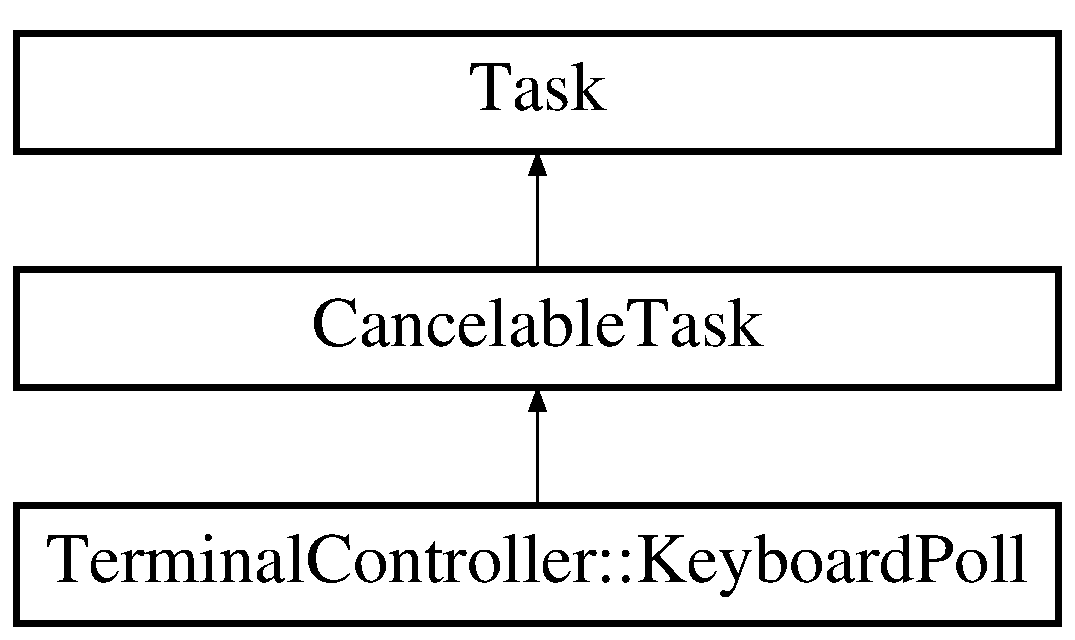
\includegraphics[height=3cm]{classTerminalController_1_1KeyboardPoll}
\end{center}
\end{figure}
\subsection*{Public Member Functions}
\begin{DoxyCompactItemize}
\item 
\hypertarget{classTerminalController_1_1KeyboardPoll_a5367155da125738f1a92d91a602390f9}{
{\bfseries KeyboardPoll} (\hyperlink{classTerminalController}{TerminalController} $\ast$controller)  throw ()}
\label{classTerminalController_1_1KeyboardPoll_a5367155da125738f1a92d91a602390f9}

\end{DoxyCompactItemize}
\subsection*{Protected Member Functions}
\begin{DoxyCompactItemize}
\item 
\hypertarget{classTerminalController_1_1KeyboardPoll_a1af4db6a3ba3b4aaabc7eb72c76b7397}{
virtual void {\bfseries real\_\-task} ()}
\label{classTerminalController_1_1KeyboardPoll_a1af4db6a3ba3b4aaabc7eb72c76b7397}

\end{DoxyCompactItemize}
\subsection*{Protected Attributes}
\begin{DoxyCompactItemize}
\item 
\hypertarget{classTerminalController_1_1KeyboardPoll_a4661060e5cf2cdabd9ba416da0d27d2c}{
\hyperlink{classTerminalController}{TerminalController} $\ast$ {\bfseries controller}}
\label{classTerminalController_1_1KeyboardPoll_a4661060e5cf2cdabd9ba416da0d27d2c}

\end{DoxyCompactItemize}


The documentation for this class was generated from the following files:\begin{DoxyCompactItemize}
\item 
terminalcontroller.h\item 
terminalcontroller.cc\end{DoxyCompactItemize}

\hypertarget{classTerminalController_1_1KeyboardRepoll}{
\section{TerminalController::KeyboardRepoll Class Reference}
\label{classTerminalController_1_1KeyboardRepoll}\index{TerminalController::KeyboardRepoll@{TerminalController::KeyboardRepoll}}
}
Inheritance diagram for TerminalController::KeyboardRepoll:\begin{figure}[H]
\begin{center}
\leavevmode
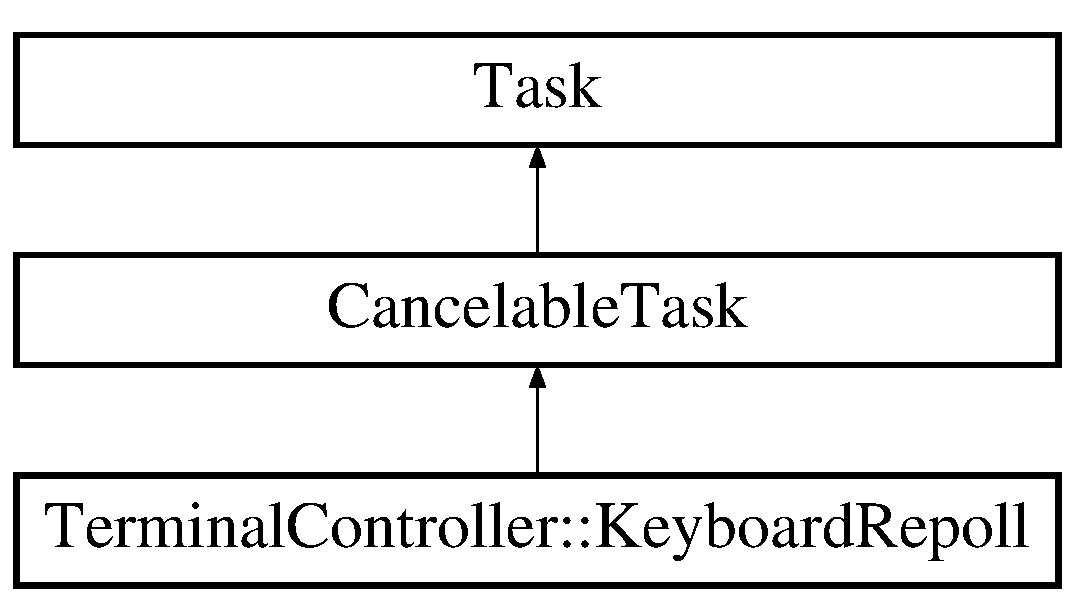
\includegraphics[height=3cm]{classTerminalController_1_1KeyboardRepoll}
\end{center}
\end{figure}
\subsection*{Public Member Functions}
\begin{DoxyCompactItemize}
\item 
\hypertarget{classTerminalController_1_1KeyboardRepoll_aaa7d42fbcac1d6ebd40798a2881e2f82}{
{\bfseries KeyboardRepoll} (\hyperlink{classTerminalController}{TerminalController} $\ast$controller, int line)  throw ()}
\label{classTerminalController_1_1KeyboardRepoll_aaa7d42fbcac1d6ebd40798a2881e2f82}

\end{DoxyCompactItemize}
\subsection*{Protected Member Functions}
\begin{DoxyCompactItemize}
\item 
\hypertarget{classTerminalController_1_1KeyboardRepoll_a4446f19f4cfa20e4bbc307ae11f575b0}{
virtual void {\bfseries real\_\-task} ()}
\label{classTerminalController_1_1KeyboardRepoll_a4446f19f4cfa20e4bbc307ae11f575b0}

\end{DoxyCompactItemize}
\subsection*{Protected Attributes}
\begin{DoxyCompactItemize}
\item 
\hypertarget{classTerminalController_1_1KeyboardRepoll_a5eadc6ba6a2de90cfba9b5f6fab7c422}{
\hyperlink{classTerminalController}{TerminalController} $\ast$ {\bfseries controller}}
\label{classTerminalController_1_1KeyboardRepoll_a5eadc6ba6a2de90cfba9b5f6fab7c422}

\item 
\hypertarget{classTerminalController_1_1KeyboardRepoll_a6625ea420771847109a74dbe775de5d4}{
int {\bfseries line}}
\label{classTerminalController_1_1KeyboardRepoll_a6625ea420771847109a74dbe775de5d4}

\end{DoxyCompactItemize}


The documentation for this class was generated from the following files:\begin{DoxyCompactItemize}
\item 
terminalcontroller.h\item 
terminalcontroller.cc\end{DoxyCompactItemize}

\hypertarget{structlast__change}{
\section{last\_\-change Struct Reference}
\label{structlast__change}\index{last\_\-change@{last\_\-change}}
}
\subsection*{Public Member Functions}
\begin{DoxyCompactItemize}
\item 
\hypertarget{structlast__change_a43a6801c6ef3c378c274a3c310d80a33}{
{\bfseries last\_\-change} (uint32 pc\_\-, uint32 instr\_\-, uint32 old\_\-value\_\-)}
\label{structlast__change_a43a6801c6ef3c378c274a3c310d80a33}

\end{DoxyCompactItemize}
\subsection*{Static Public Member Functions}
\begin{DoxyCompactItemize}
\item 
\hypertarget{structlast__change_a8371a85941a88825f636d36a56a22d28}{
static \hyperlink{structlast__change}{last\_\-change} {\bfseries make} (uint32 pc\_\-, uint32 instr\_\-, uint32 old\_\-value\_\-)}
\label{structlast__change_a8371a85941a88825f636d36a56a22d28}

\end{DoxyCompactItemize}
\subsection*{Public Attributes}
\begin{DoxyCompactItemize}
\item 
\hypertarget{structlast__change_abfd79bca221e524bc0b231e0fadcef16}{
uint32 {\bfseries pc}}
\label{structlast__change_abfd79bca221e524bc0b231e0fadcef16}

\item 
\hypertarget{structlast__change_a7e56a184561e0f3b18732d3f559ce14d}{
uint32 {\bfseries instr}}
\label{structlast__change_a7e56a184561e0f3b18732d3f559ce14d}

\item 
\hypertarget{structlast__change_aeb39258427782c5df01510ff10a0b328}{
uint32 {\bfseries old\_\-value}}
\label{structlast__change_aeb39258427782c5df01510ff10a0b328}

\end{DoxyCompactItemize}


The documentation for this struct was generated from the following file:\begin{DoxyCompactItemize}
\item 
cpu.h\end{DoxyCompactItemize}

\hypertarget{structTerminalController_1_1LineState}{
\section{TerminalController::LineState Struct Reference}
\label{structTerminalController_1_1LineState}\index{TerminalController::LineState@{TerminalController::LineState}}
}
\subsection*{Public Attributes}
\begin{DoxyCompactItemize}
\item 
\hypertarget{structTerminalController_1_1LineState_aa3d5368683cf0c21a6eb4d995a7a0d76}{
termios {\bfseries tty\_\-state}}
\label{structTerminalController_1_1LineState_aa3d5368683cf0c21a6eb4d995a7a0d76}

\item 
\hypertarget{structTerminalController_1_1LineState_aa6ed05eb943bb04a902a0c10cbb4c98b}{
int {\bfseries tty\_\-fd}}
\label{structTerminalController_1_1LineState_aa6ed05eb943bb04a902a0c10cbb4c98b}

\item 
\hypertarget{structTerminalController_1_1LineState_a88e46fd3d83878ce3d92d85a245796e8}{
\hyperlink{classTerminalController_1_1KeyboardRepoll}{KeyboardRepoll} $\ast$ {\bfseries keyboard\_\-repoll}}
\label{structTerminalController_1_1LineState_a88e46fd3d83878ce3d92d85a245796e8}

\item 
\hypertarget{structTerminalController_1_1LineState_a478b3bef98dd7e10aa79f71d88c29c64}{
\hyperlink{classTerminalController_1_1DisplayDelay}{DisplayDelay} $\ast$ {\bfseries display\_\-delay}}
\label{structTerminalController_1_1LineState_a478b3bef98dd7e10aa79f71d88c29c64}

\item 
\hypertarget{structTerminalController_1_1LineState_a6f28f0977415d283fb1cf51935fc4388}{
char {\bfseries keyboard\_\-char}}
\label{structTerminalController_1_1LineState_a6f28f0977415d283fb1cf51935fc4388}

\item 
\hypertarget{structTerminalController_1_1LineState_aa6e0e680ed2f77007c03f870a21b6bb0}{
State {\bfseries keyboard\_\-state}}
\label{structTerminalController_1_1LineState_aa6e0e680ed2f77007c03f870a21b6bb0}

\item 
\hypertarget{structTerminalController_1_1LineState_aa477be2fd952f2218d951ff2ee5c63db}{
State {\bfseries display\_\-state}}
\label{structTerminalController_1_1LineState_aa477be2fd952f2218d951ff2ee5c63db}

\end{DoxyCompactItemize}


The documentation for this struct was generated from the following file:\begin{DoxyCompactItemize}
\item 
terminalcontroller.h\end{DoxyCompactItemize}

\hypertarget{classPlog_1_1Log}{
\section{Plog::Log Class Reference}
\label{classPlog_1_1Log}\index{Plog::Log@{Plog::Log}}
}
\subsection*{Static Public Member Functions}
\begin{DoxyCompactItemize}
\item 
\hypertarget{classPlog_1_1Log_a4881c1fa2a0fc05d439cbc246cfd4743}{
static bool {\bfseries ShouldLog} (\hyperlink{classPlog_1_1CallSite}{CallSite} \&)}
\label{classPlog_1_1Log_a4881c1fa2a0fc05d439cbc246cfd4743}

\item 
\hypertarget{classPlog_1_1Log_a0d7251048b9f8b3998366e9a283b9547}{
static std::ostringstream $\ast$ {\bfseries Out} ()}
\label{classPlog_1_1Log_a0d7251048b9f8b3998366e9a283b9547}

\item 
\hypertarget{classPlog_1_1Log_abbadf43bf9aae54fb93ed366800deb19}{
static void {\bfseries Flush} (std::ostringstream $\ast$, const \hyperlink{classPlog_1_1CallSite}{CallSite} \&)}
\label{classPlog_1_1Log_abbadf43bf9aae54fb93ed366800deb19}

\end{DoxyCompactItemize}


The documentation for this class was generated from the following files:\begin{DoxyCompactItemize}
\item 
prophetlog.h\item 
prophetlog.cc\end{DoxyCompactItemize}

\hypertarget{classMapper}{
\section{Mapper Class Reference}
\label{classMapper}\index{Mapper@{Mapper}}
}
\subsection*{Classes}
\begin{DoxyCompactItemize}
\item 
struct \hyperlink{structMapper_1_1BusErrorInfo}{BusErrorInfo}
\end{DoxyCompactItemize}
\subsection*{Public Types}
\begin{DoxyCompactItemize}
\item 
\hypertarget{classMapper_a70bf3035f1c02611e55f05dfa7a80187}{
typedef std::vector$<$ \hyperlink{classRange}{Range} $\ast$ $>$ {\bfseries Ranges}}
\label{classMapper_a70bf3035f1c02611e55f05dfa7a80187}

\end{DoxyCompactItemize}
\subsection*{Public Member Functions}
\begin{DoxyCompactItemize}
\item 
\hypertarget{classMapper_a8733fffed63e13e9a0584d2e3c85d0b4}{
int {\bfseries add\_\-range} (\hyperlink{classRange}{Range} $\ast$r)}
\label{classMapper_a8733fffed63e13e9a0584d2e3c85d0b4}

\item 
\hypertarget{classMapper_a1c30883b6490a8283f4dab8dfe797860}{
int {\bfseries map\_\-at\_\-physical\_\-address} (\hyperlink{classRange}{Range} $\ast$r, uint32 pa)}
\label{classMapper_a1c30883b6490a8283f4dab8dfe797860}

\item 
\hypertarget{classMapper_aad996f69d0a2aca785f5a8e9440789be}{
uint32 {\bfseries swap\_\-word} (uint32 w)}
\label{classMapper_aad996f69d0a2aca785f5a8e9440789be}

\item 
\hypertarget{classMapper_a51a9d4d84550d699fa738fccc0e227da}{
uint16 {\bfseries swap\_\-halfword} (uint16 h)}
\label{classMapper_a51a9d4d84550d699fa738fccc0e227da}

\item 
\hypertarget{classMapper_ac40b7a8813b99b8b71ac2ae9e18c07b6}{
uint32 {\bfseries mips\_\-to\_\-host\_\-word} (uint32 w)}
\label{classMapper_ac40b7a8813b99b8b71ac2ae9e18c07b6}

\item 
\hypertarget{classMapper_ab63092a89802fab46fe3c4e2191e76fd}{
uint32 {\bfseries host\_\-to\_\-mips\_\-word} (uint32 w)}
\label{classMapper_ab63092a89802fab46fe3c4e2191e76fd}

\item 
\hypertarget{classMapper_a071b247e7dc9ec05844a168dba047b85}{
uint16 {\bfseries mips\_\-to\_\-host\_\-halfword} (uint16 h)}
\label{classMapper_a071b247e7dc9ec05844a168dba047b85}

\item 
\hypertarget{classMapper_a18be0c1a96acac7cea7b32b9d46ba800}{
uint16 {\bfseries host\_\-to\_\-mips\_\-halfword} (uint16 h)}
\label{classMapper_a18be0c1a96acac7cea7b32b9d46ba800}

\item 
\hypertarget{classMapper_a79b29cfdb440f48772303d66c8f33ad1}{
void {\bfseries bus\_\-error} (\hyperlink{classDeviceExc}{DeviceExc} $\ast$client, int32 mode, uint32 addr, int32 width, uint32 data=0xffffffff)}
\label{classMapper_a79b29cfdb440f48772303d66c8f33ad1}

\item 
\hypertarget{classMapper_a4633b1f7ac51dfac73feff2fc4cc24e9}{
uint32 {\bfseries fetch\_\-word} (uint32 addr, int32 mode, bool cacheable, \hyperlink{classDeviceExc}{DeviceExc} $\ast$client)}
\label{classMapper_a4633b1f7ac51dfac73feff2fc4cc24e9}

\item 
\hypertarget{classMapper_a89eff1600c368db94fcd2cfecccc3d30}{
uint16 {\bfseries fetch\_\-halfword} (uint32 addr, bool cacheable, \hyperlink{classDeviceExc}{DeviceExc} $\ast$client)}
\label{classMapper_a89eff1600c368db94fcd2cfecccc3d30}

\item 
\hypertarget{classMapper_a8992f22898fce1355d26c9920fc0fd04}{
uint8 {\bfseries fetch\_\-byte} (uint32 addr, bool cacheable, \hyperlink{classDeviceExc}{DeviceExc} $\ast$client)}
\label{classMapper_a8992f22898fce1355d26c9920fc0fd04}

\item 
\hypertarget{classMapper_a7d9aef8d094254baf1a629ce7ac87366}{
void {\bfseries store\_\-word} (uint32 addr, uint32 data, bool cacheable, \hyperlink{classDeviceExc}{DeviceExc} $\ast$client)}
\label{classMapper_a7d9aef8d094254baf1a629ce7ac87366}

\item 
\hypertarget{classMapper_acc43182e1ae60925793b36ba7c35dbfd}{
void {\bfseries store\_\-halfword} (uint32 addr, uint16 data, bool cacheable, \hyperlink{classDeviceExc}{DeviceExc} $\ast$client)}
\label{classMapper_acc43182e1ae60925793b36ba7c35dbfd}

\item 
\hypertarget{classMapper_a161265d93e767b5e52fbfb4d83970f87}{
void {\bfseries store\_\-byte} (uint32 addr, uint8 data, bool cacheable, \hyperlink{classDeviceExc}{DeviceExc} $\ast$client)}
\label{classMapper_a161265d93e767b5e52fbfb4d83970f87}

\item 
\hypertarget{classMapper_af8ef34c52d4c0fdf5f5e7c12587cf455}{
\hyperlink{classRange}{Range} $\ast$ {\bfseries find\_\-mapping\_\-range} (uint32 p)  throw ()}
\label{classMapper_af8ef34c52d4c0fdf5f5e7c12587cf455}

\item 
\hypertarget{classMapper_ab77d2b3eea937495e705aaba009b3940}{
void {\bfseries dump\_\-stack} (FILE $\ast$f, uint32 stackphys)}
\label{classMapper_ab77d2b3eea937495e705aaba009b3940}

\item 
\hypertarget{classMapper_afe775b5a9960a04b565bc851755bb6e4}{
void {\bfseries get\_\-last\_\-berr\_\-info} (\hyperlink{structMapper_1_1BusErrorInfo}{BusErrorInfo} \&info)}
\label{classMapper_afe775b5a9960a04b565bc851755bb6e4}

\end{DoxyCompactItemize}
\subsection*{Public Attributes}
\begin{DoxyCompactItemize}
\item 
\hypertarget{classMapper_a0a22497e194768c9324d2b91d5d4d5af}{
\hyperlink{structMapper_1_1BusErrorInfo}{BusErrorInfo} {\bfseries last\_\-berr\_\-info}}
\label{classMapper_a0a22497e194768c9324d2b91d5d4d5af}

\end{DoxyCompactItemize}


The documentation for this class was generated from the following files:\begin{DoxyCompactItemize}
\item 
mapper.h\item 
mapper.cc\end{DoxyCompactItemize}

\hypertarget{classMemoryModule}{
\section{MemoryModule Class Reference}
\label{classMemoryModule}\index{MemoryModule@{MemoryModule}}
}
Inheritance diagram for MemoryModule:\begin{figure}[H]
\begin{center}
\leavevmode
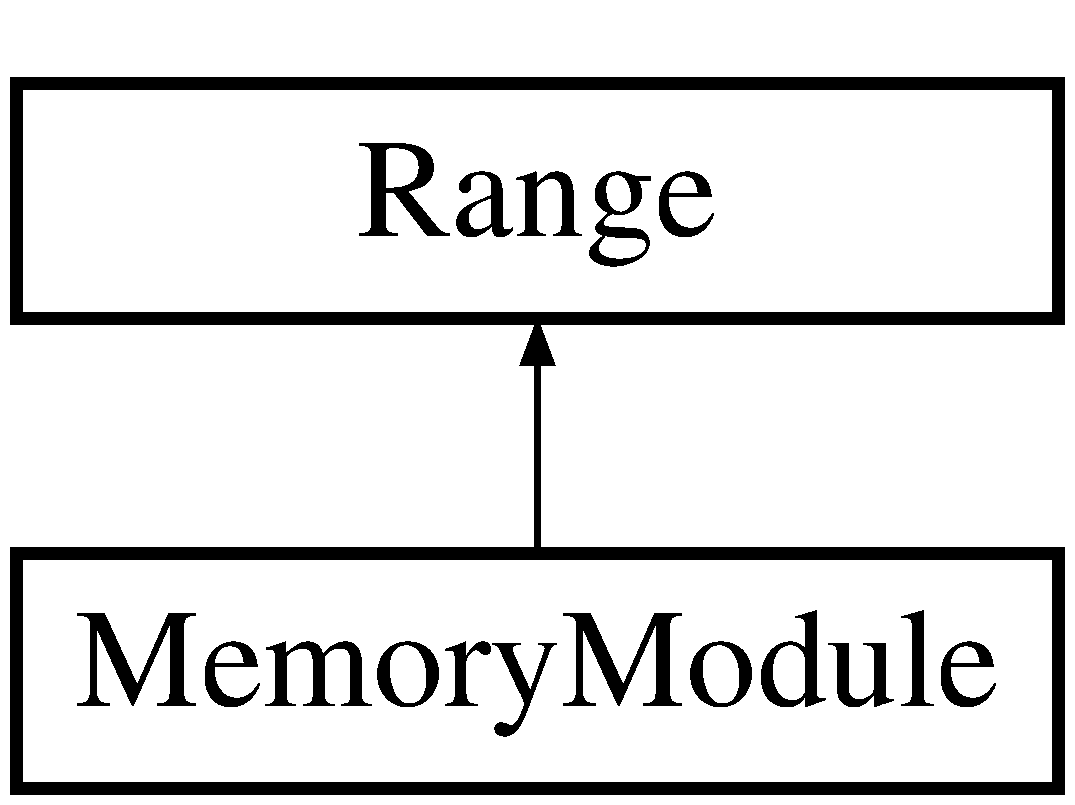
\includegraphics[height=2cm]{classMemoryModule}
\end{center}
\end{figure}
\subsection*{Public Member Functions}
\begin{DoxyCompactItemize}
\item 
\hypertarget{classMemoryModule_a6d75820f2b0187421938e5a54d016c81}{
{\bfseries MemoryModule} (size\_\-t size)}
\label{classMemoryModule_a6d75820f2b0187421938e5a54d016c81}

\end{DoxyCompactItemize}
\subsection*{Public Attributes}
\begin{DoxyCompactItemize}
\item 
\hypertarget{classMemoryModule_a61b35d32fd4ca055aa41d7665baa3c87}{
uint32 $\ast$ {\bfseries myaddr}}
\label{classMemoryModule_a61b35d32fd4ca055aa41d7665baa3c87}

\end{DoxyCompactItemize}


The documentation for this class was generated from the following file:\begin{DoxyCompactItemize}
\item 
memorymodule.h\end{DoxyCompactItemize}

\hypertarget{classPlog_1_1NoClassInfo}{
\section{Plog::NoClassInfo Class Reference}
\label{classPlog_1_1NoClassInfo}\index{Plog::NoClassInfo@{Plog::NoClassInfo}}
}


The documentation for this class was generated from the following file:\begin{DoxyCompactItemize}
\item 
prophetlog.h\end{DoxyCompactItemize}

\hypertarget{structTrace_1_1Operand}{
\section{Trace::Operand Struct Reference}
\label{structTrace_1_1Operand}\index{Trace::Operand@{Trace::Operand}}
}
\subsection*{Public Member Functions}
\begin{DoxyCompactItemize}
\item 
\hypertarget{structTrace_1_1Operand_a4d3d267d61dbcd7b7908c422b4172638}{
{\bfseries Operand} (const char $\ast$tag\_\-, int regno\_\-, uint32 val\_\-)}
\label{structTrace_1_1Operand_a4d3d267d61dbcd7b7908c422b4172638}

\item 
\hypertarget{structTrace_1_1Operand_ad0114607af6885d946620aef2490febf}{
{\bfseries Operand} (const char $\ast$tag\_\-, uint32 val\_\-)}
\label{structTrace_1_1Operand_ad0114607af6885d946620aef2490febf}

\end{DoxyCompactItemize}
\subsection*{Static Public Member Functions}
\begin{DoxyCompactItemize}
\item 
\hypertarget{structTrace_1_1Operand_a447d15d9296741d1932284be020a7e72}{
static \hyperlink{structTrace_1_1Operand}{Operand} {\bfseries make} (const char $\ast$tag\_\-, int regno\_\-, uint32 val\_\-)}
\label{structTrace_1_1Operand_a447d15d9296741d1932284be020a7e72}

\item 
\hypertarget{structTrace_1_1Operand_a8907c7fe05eb0bd1e770ea3a246b59e1}{
static \hyperlink{structTrace_1_1Operand}{Operand} {\bfseries make} (const char $\ast$tag\_\-, uint32 val\_\-)}
\label{structTrace_1_1Operand_a8907c7fe05eb0bd1e770ea3a246b59e1}

\end{DoxyCompactItemize}
\subsection*{Public Attributes}
\begin{DoxyCompactItemize}
\item 
\hypertarget{structTrace_1_1Operand_a9b796de2fc78d642b7330745c2d8a520}{
const char $\ast$ {\bfseries tag}}
\label{structTrace_1_1Operand_a9b796de2fc78d642b7330745c2d8a520}

\item 
\hypertarget{structTrace_1_1Operand_a6c025207b70e102cb5338258d709136e}{
int {\bfseries regno}}
\label{structTrace_1_1Operand_a6c025207b70e102cb5338258d709136e}

\item 
\hypertarget{structTrace_1_1Operand_a551b2f8b156c890c2399f04d8d9dfefb}{
uint32 {\bfseries val}}
\label{structTrace_1_1Operand_a551b2f8b156c890c2399f04d8d9dfefb}

\end{DoxyCompactItemize}


The documentation for this struct was generated from the following file:\begin{DoxyCompactItemize}
\item 
cpu.h\end{DoxyCompactItemize}

\hypertarget{structOption}{
\section{Option Struct Reference}
\label{structOption}\index{Option@{Option}}
}
\subsection*{Public Attributes}
\begin{DoxyCompactItemize}
\item 
\hypertarget{structOption_a8aae24492e599aeb657d5f953044196c}{
char $\ast$ {\bfseries name}}
\label{structOption_a8aae24492e599aeb657d5f953044196c}

\item 
\hypertarget{structOption_a6cfb977fc319239971836988f5f665dc}{
int {\bfseries type}}
\label{structOption_a6cfb977fc319239971836988f5f665dc}

\item 
\hypertarget{structOption_ac5691f09bc79d4185da7d88730f53b62}{
union \hyperlink{unionOptionValue}{OptionValue} {\bfseries value}}
\label{structOption_ac5691f09bc79d4185da7d88730f53b62}

\end{DoxyCompactItemize}


The documentation for this struct was generated from the following file:\begin{DoxyCompactItemize}
\item 
options.h\end{DoxyCompactItemize}

\hypertarget{classOptions}{
\section{Options Class Reference}
\label{classOptions}\index{Options@{Options}}
}
Inheritance diagram for Options:\begin{figure}[H]
\begin{center}
\leavevmode
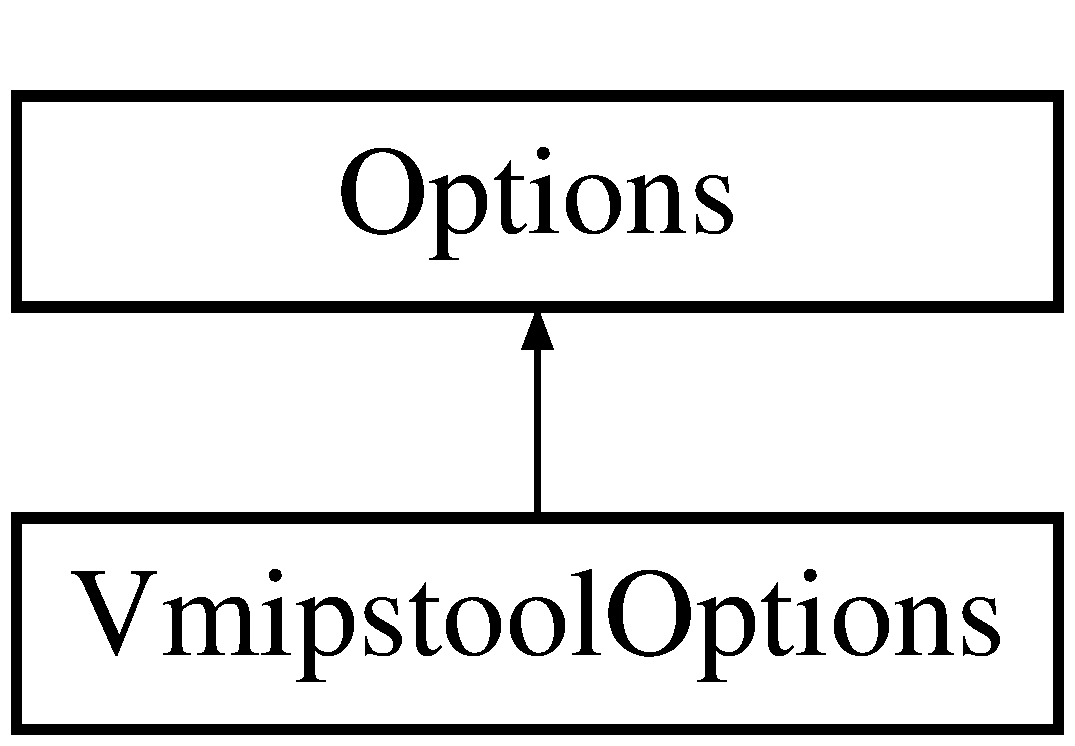
\includegraphics[height=2cm]{classOptions}
\end{center}
\end{figure}
\subsection*{Public Member Functions}
\begin{DoxyCompactItemize}
\item 
\hypertarget{classOptions_a3bcfc6315059cdfc80086ac4e8ebb8fb}{
virtual void {\bfseries process\_\-options} (int argc, char $\ast$$\ast$argv)}
\label{classOptions_a3bcfc6315059cdfc80086ac4e8ebb8fb}

\item 
\hypertarget{classOptions_a3a535c4c76588d00f62c9817bc0ff63b}{
union \hyperlink{unionOptionValue}{OptionValue} $\ast$ {\bfseries option} (char $\ast$name)}
\label{classOptions_a3a535c4c76588d00f62c9817bc0ff63b}

\end{DoxyCompactItemize}
\subsection*{Protected Types}
\begin{DoxyCompactItemize}
\item 
\hypertarget{classOptions_af9c17aca9b06a52a376735f3985613a2}{
typedef std::map$<$ std::string, \hyperlink{structOption}{Option} $>$ {\bfseries OptionMap}}
\label{classOptions_af9c17aca9b06a52a376735f3985613a2}

\end{DoxyCompactItemize}
\subsection*{Protected Member Functions}
\begin{DoxyCompactItemize}
\item 
\hypertarget{classOptions_a5b2d7759ab32fe3a5c638a18862a0e54}{
void {\bfseries process\_\-defaults} (void)}
\label{classOptions_a5b2d7759ab32fe3a5c638a18862a0e54}

\item 
\hypertarget{classOptions_ad8ec1474331ba97df748a9ceaf1f48a6}{
void {\bfseries process\_\-one\_\-option} (const char $\ast$const option)}
\label{classOptions_ad8ec1474331ba97df748a9ceaf1f48a6}

\item 
\hypertarget{classOptions_a76a5fec3abf24dd992b76e6056392604}{
int {\bfseries process\_\-first\_\-option} (char $\ast$$\ast$bufptr, int lineno=0, char $\ast$fn=NULL)}
\label{classOptions_a76a5fec3abf24dd992b76e6056392604}

\item 
\hypertarget{classOptions_a06b815b611cffcd3ee17fdaeb1787854}{
int {\bfseries process\_\-options\_\-from\_\-file} (char $\ast$filename)}
\label{classOptions_a06b815b611cffcd3ee17fdaeb1787854}

\item 
\hypertarget{classOptions_af82c0bbc02cb2c8f6a115dd1fdd43579}{
int {\bfseries tilde\_\-expand} (char $\ast$filename)}
\label{classOptions_af82c0bbc02cb2c8f6a115dd1fdd43579}

\item 
\hypertarget{classOptions_a50a9e19f3ff310d8d483dc74d4442a87}{
virtual void {\bfseries usage} (char $\ast$argv0)}
\label{classOptions_a50a9e19f3ff310d8d483dc74d4442a87}

\item 
\hypertarget{classOptions_a6e6c73b2ed51467f7f076638e0726629}{
void {\bfseries set\_\-str\_\-option} (char $\ast$key, char $\ast$value)}
\label{classOptions_a6e6c73b2ed51467f7f076638e0726629}

\item 
\hypertarget{classOptions_ab7f5346ac22e0c72eafb3324fd84236e}{
void {\bfseries set\_\-num\_\-option} (char $\ast$key, uint32 value)}
\label{classOptions_ab7f5346ac22e0c72eafb3324fd84236e}

\item 
\hypertarget{classOptions_a89174e246a138fd030eed58a2ca2f358}{
void {\bfseries set\_\-flag\_\-option} (char $\ast$key, bool value)}
\label{classOptions_a89174e246a138fd030eed58a2ca2f358}

\item 
\hypertarget{classOptions_a1273ec7b1f585443952d3d43feec0010}{
char $\ast$ {\bfseries strprefix} (char $\ast$crack\_\-smoker, char $\ast$crack)}
\label{classOptions_a1273ec7b1f585443952d3d43feec0010}

\item 
\hypertarget{classOptions_a43c1b070c853edd7d3b227e300f6db80}{
int {\bfseries find\_\-option\_\-type} (char $\ast$option)}
\label{classOptions_a43c1b070c853edd7d3b227e300f6db80}

\item 
\hypertarget{classOptions_a4a9be4a96d5b12a8abb469fef02af7ee}{
\hyperlink{structOption}{Option} $\ast$ {\bfseries optstruct} (char $\ast$name, bool install=false)}
\label{classOptions_a4a9be4a96d5b12a8abb469fef02af7ee}

\item 
\hypertarget{classOptions_a11e86765e4e309f8eb0abef4f235d106}{
void {\bfseries print\_\-package\_\-version} (char $\ast$toolname, char $\ast$version)}
\label{classOptions_a11e86765e4e309f8eb0abef4f235d106}

\item 
\hypertarget{classOptions_ac6c9b11dab112ef2647386e45da45bb0}{
void {\bfseries print\_\-config\_\-info} (void)}
\label{classOptions_ac6c9b11dab112ef2647386e45da45bb0}

\end{DoxyCompactItemize}
\subsection*{Protected Attributes}
\begin{DoxyCompactItemize}
\item 
\hypertarget{classOptions_a9c57c93eb164dd69a2c63c8d86f90ab2}{
OptionMap {\bfseries table}}
\label{classOptions_a9c57c93eb164dd69a2c63c8d86f90ab2}

\end{DoxyCompactItemize}


The documentation for this class was generated from the following files:\begin{DoxyCompactItemize}
\item 
options.h\item 
options.cc\end{DoxyCompactItemize}

\hypertarget{unionOptionValue}{
\section{OptionValue Union Reference}
\label{unionOptionValue}\index{OptionValue@{OptionValue}}
}
\subsection*{Public Attributes}
\begin{DoxyCompactItemize}
\item 
\hypertarget{unionOptionValue_a80ecb0b3cfc92d6b6d4fdf1d958a6017}{
char $\ast$ {\bfseries str}}
\label{unionOptionValue_a80ecb0b3cfc92d6b6d4fdf1d958a6017}

\item 
\hypertarget{unionOptionValue_a755d65b9d23c7e92f1168787208a4f51}{
bool {\bfseries flag}}
\label{unionOptionValue_a755d65b9d23c7e92f1168787208a4f51}

\item 
\hypertarget{unionOptionValue_aef8f2590401c87928a7565885e3633fc}{
uint32 {\bfseries num}}
\label{unionOptionValue_aef8f2590401c87928a7565885e3633fc}

\end{DoxyCompactItemize}


The documentation for this union was generated from the following file:\begin{DoxyCompactItemize}
\item 
options.h\end{DoxyCompactItemize}

\hypertarget{classProphet}{
\section{Prophet Class Reference}
\label{classProphet}\index{Prophet@{Prophet}}
}
Inheritance diagram for Prophet:\begin{figure}[H]
\begin{center}
\leavevmode
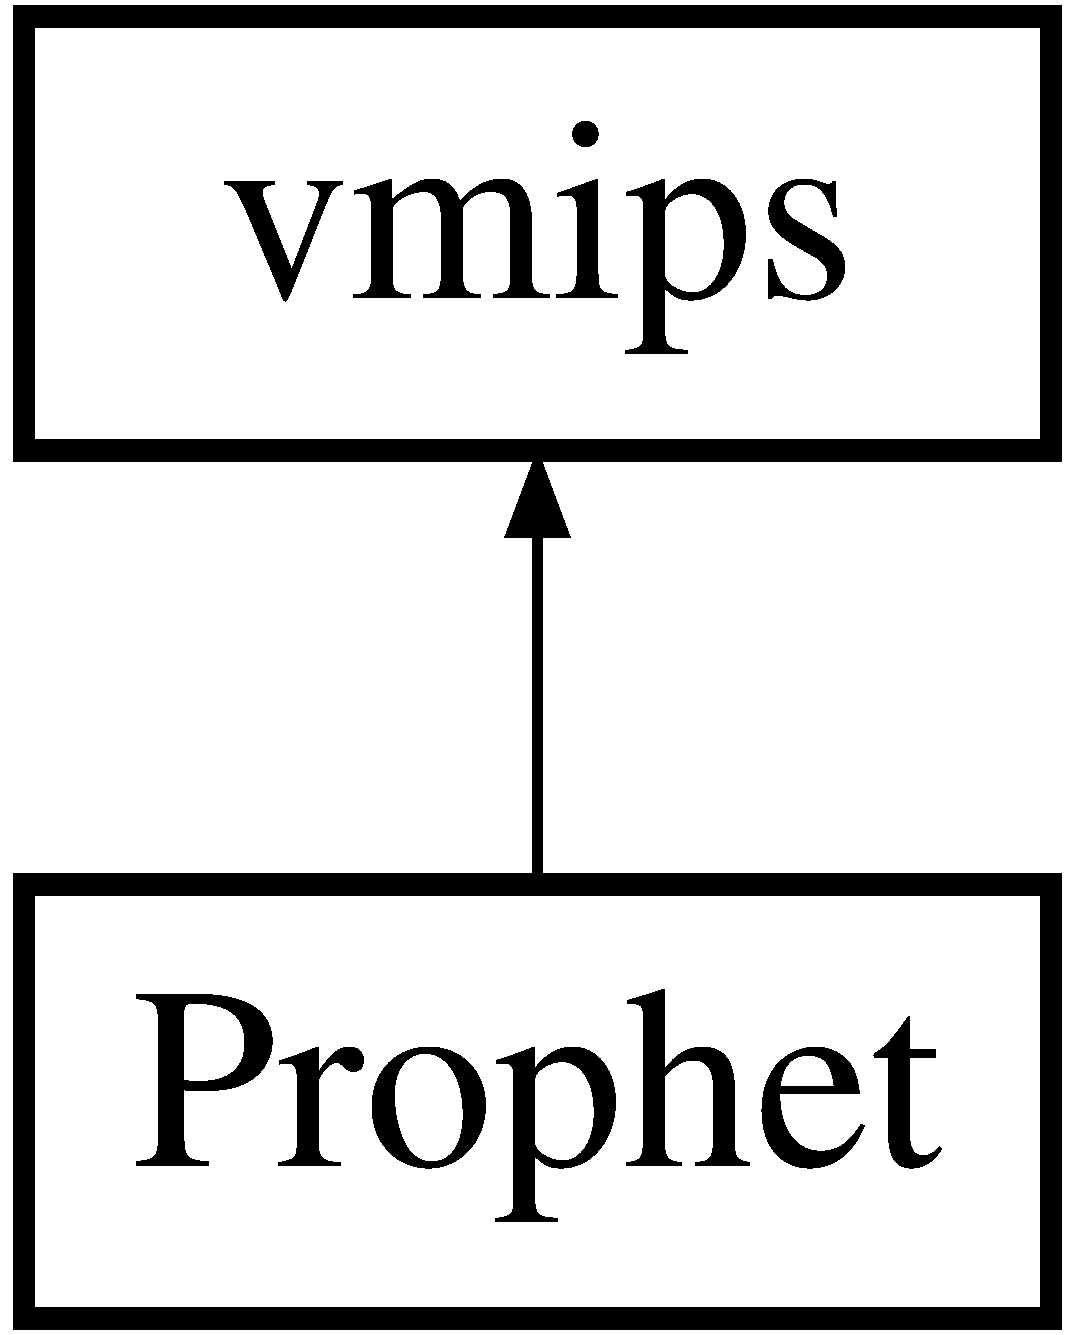
\includegraphics[height=2cm]{classProphet}
\end{center}
\end{figure}
\subsection*{Public Member Functions}
\begin{DoxyCompactItemize}
\item 
\hypertarget{classProphet_a57c6fa39fd79cacf5628304f85684139}{
{\bfseries Prophet} (uint32 argc, char $\ast$$\ast$argv)}
\label{classProphet_a57c6fa39fd79cacf5628304f85684139}

\item 
\hypertarget{classProphet_ae68eeb183488d3b2bd747e94ef28bc79}{
void {\bfseries setup\_\-machine} (void)}
\label{classProphet_ae68eeb183488d3b2bd747e94ef28bc79}

\item 
\hypertarget{classProphet_a268003f7e2637a524dfe893c9ca27089}{
void {\bfseries step} (void)}
\label{classProphet_a268003f7e2637a524dfe893c9ca27089}

\item 
\hypertarget{classProphet_abb3b6f1777aadb0a5b40c38a56ca36b9}{
int {\bfseries run} (void)}
\label{classProphet_abb3b6f1777aadb0a5b40c38a56ca36b9}

\item 
\hypertarget{classProphet_abe7eb928d0f643a21bc77c2db533ad63}{
uint32 {\bfseries getCpuNum} ()}
\label{classProphet_abe7eb928d0f643a21bc77c2db533ad63}

\end{DoxyCompactItemize}


The documentation for this class was generated from the following files:\begin{DoxyCompactItemize}
\item 
prophet\_\-vmips.h\item 
prophet\_\-vmips.cc\end{DoxyCompactItemize}

\hypertarget{classProphetStat_1_1ProphetCpuStat}{
\section{ProphetStat::ProphetCpuStat Class Reference}
\label{classProphetStat_1_1ProphetCpuStat}\index{ProphetStat::ProphetCpuStat@{ProphetStat::ProphetCpuStat}}
}


{\ttfamily \#include $<$prophetcpustat.h$>$}

\subsection*{Public Member Functions}
\begin{DoxyCompactItemize}
\item 
void \hyperlink{classProphetStat_1_1ProphetCpuStat_a80086134fec10a5180c7c7a2c3cc2378}{addSquashLen} (int cpuId, int len)
\item 
void \hyperlink{classProphetStat_1_1ProphetCpuStat_ae57688a78d61dcbe7370fefae03ecb98}{addProCpuStatToXml} (\hyperlink{classXmlElement}{XmlElement} $\ast$root)
\item 
void \hyperlink{classProphetStat_1_1ProphetCpuStat_a8343c003cef10d15351dbafcfc74962e}{printCpuStat} (FILE $\ast$fp=stderr)
\item 
\hypertarget{classProphetStat_1_1ProphetCpuStat_acd041425cbc0d744751b87a121047ab9}{
\hyperlink{classProphetStat_1_1SquashOnSpList}{SquashOnSpList} $\ast$ {\bfseries getSquList} ()}
\label{classProphetStat_1_1ProphetCpuStat_acd041425cbc0d744751b87a121047ab9}

\end{DoxyCompactItemize}
\subsection*{Static Public Member Functions}
\begin{DoxyCompactItemize}
\item 
static \hyperlink{classProphetStat_1_1ProphetCpuStat}{ProphetCpuStat} $\ast$ \hyperlink{classProphetStat_1_1ProphetCpuStat_a1dfee1a62c17b8e9035b68563368702e}{getProCpuStatInstance} ()
\end{DoxyCompactItemize}
\subsection*{Static Public Attributes}
\begin{DoxyCompactItemize}
\item 
\hypertarget{classProphetStat_1_1ProphetCpuStat_aa86b6ecd1908f2dcb64aa4c016758d81}{
static int {\bfseries coreNum} = 0}
\label{classProphetStat_1_1ProphetCpuStat_aa86b6ecd1908f2dcb64aa4c016758d81}

\end{DoxyCompactItemize}
\subsection*{Protected Member Functions}
\begin{DoxyCompactItemize}
\item 
\hypertarget{classProphetStat_1_1ProphetCpuStat_ad9e5aad82ee6015568bdfa6f3417458e}{
void {\bfseries getTotalSquashLen} ()}
\label{classProphetStat_1_1ProphetCpuStat_ad9e5aad82ee6015568bdfa6f3417458e}

\item 
\hypertarget{classProphetStat_1_1ProphetCpuStat_a515c271e82770fa4155b9aa30e6e6bf6}{
void {\bfseries printSquashLen} (FILE $\ast$fp=stderr)}
\label{classProphetStat_1_1ProphetCpuStat_a515c271e82770fa4155b9aa30e6e6bf6}

\item 
\hypertarget{classProphetStat_1_1ProphetCpuStat_ae07ae8a7fe5a86b18e4916673f5f8d0f}{
void {\bfseries addSquashLenToXml} (\hyperlink{classXmlElement}{XmlElement} $\ast$root)}
\label{classProphetStat_1_1ProphetCpuStat_ae07ae8a7fe5a86b18e4916673f5f8d0f}

\end{DoxyCompactItemize}


\subsection{Detailed Description}
cpustat class 

\subsection{Member Function Documentation}
\hypertarget{classProphetStat_1_1ProphetCpuStat_ae57688a78d61dcbe7370fefae03ecb98}{
\index{ProphetStat::ProphetCpuStat@{ProphetStat::ProphetCpuStat}!addProCpuStatToXml@{addProCpuStatToXml}}
\index{addProCpuStatToXml@{addProCpuStatToXml}!ProphetStat::ProphetCpuStat@{ProphetStat::ProphetCpuStat}}
\subsubsection[{addProCpuStatToXml}]{\setlength{\rightskip}{0pt plus 5cm}void ProphetStat::ProphetCpuStat::addProCpuStatToXml ({\bf XmlElement} $\ast$ {\em root})}}
\label{classProphetStat_1_1ProphetCpuStat_ae57688a78d61dcbe7370fefae03ecb98}
将ProphetCpuStat对象统计的信息加入到root元素下,(供统一打印) 
\begin{DoxyParams}{Parameters}
\item[{\em root}](代挂载的XmlElement元素指针) \end{DoxyParams}
\hypertarget{classProphetStat_1_1ProphetCpuStat_a80086134fec10a5180c7c7a2c3cc2378}{
\index{ProphetStat::ProphetCpuStat@{ProphetStat::ProphetCpuStat}!addSquashLen@{addSquashLen}}
\index{addSquashLen@{addSquashLen}!ProphetStat::ProphetCpuStat@{ProphetStat::ProphetCpuStat}}
\subsubsection[{addSquashLen}]{\setlength{\rightskip}{0pt plus 5cm}void ProphetStat::ProphetCpuStat::addSquashLen (int {\em cpuId}, \/  int {\em len})}}
\label{classProphetStat_1_1ProphetCpuStat_a80086134fec10a5180c7c7a2c3cc2378}
将核号为cpuid上的撤销长度为len的统计值加一 
\begin{DoxyParams}{Parameters}
\item[{\em cpuId}]核号\mbox{[}0..coreNum-\/1\mbox{]} \item[{\em len}]撤销长度(此次撤销总共撤销的线程数 ) \mbox{[}0..coreNum-\/1\mbox{]} \end{DoxyParams}
\hypertarget{classProphetStat_1_1ProphetCpuStat_a1dfee1a62c17b8e9035b68563368702e}{
\index{ProphetStat::ProphetCpuStat@{ProphetStat::ProphetCpuStat}!getProCpuStatInstance@{getProCpuStatInstance}}
\index{getProCpuStatInstance@{getProCpuStatInstance}!ProphetStat::ProphetCpuStat@{ProphetStat::ProphetCpuStat}}
\subsubsection[{getProCpuStatInstance}]{\setlength{\rightskip}{0pt plus 5cm}{\bf ProphetCpuStat} $\ast$ ProphetStat::ProphetCpuStat::getProCpuStatInstance ()\hspace{0.3cm}{\ttfamily  \mbox{[}static\mbox{]}}}}
\label{classProphetStat_1_1ProphetCpuStat_a1dfee1a62c17b8e9035b68563368702e}
单例模式, 调用该静态方法返回唯一的ProphetCpuStat对象。在返回该对象前, 将coreNum的值设为 用户在运行时附带的参数的值. \begin{DoxyReturn}{Returns}
返回指向ProphetCpuStat对象的指针. 
\end{DoxyReturn}
\hypertarget{classProphetStat_1_1ProphetCpuStat_a8343c003cef10d15351dbafcfc74962e}{
\index{ProphetStat::ProphetCpuStat@{ProphetStat::ProphetCpuStat}!printCpuStat@{printCpuStat}}
\index{printCpuStat@{printCpuStat}!ProphetStat::ProphetCpuStat@{ProphetStat::ProphetCpuStat}}
\subsubsection[{printCpuStat}]{\setlength{\rightskip}{0pt plus 5cm}void ProphetStat::ProphetCpuStat::printCpuStat (FILE $\ast$ {\em fp} = {\ttfamily stderr})}}
\label{classProphetStat_1_1ProphetCpuStat_a8343c003cef10d15351dbafcfc74962e}
向文件fp 打印出ProphetCpuStat对象统计的信息.fp 指向的为普通文本文件.调用此方法时, fp 为NULL, 或stderr, 或stdout, 其他的fp不接受。当fp 为NULL使, 由方法的实现决定 创建一个新文件, 并将fp指针指向该文件. 
\begin{DoxyParams}{Parameters}
\item[{\em fp}]\end{DoxyParams}


The documentation for this class was generated from the following files:\begin{DoxyCompactItemize}
\item 
prophetcpustat.h\item 
prophetcpustat.cc\end{DoxyCompactItemize}

\hypertarget{classProphetException}{
\section{ProphetException Class Reference}
\label{classProphetException}\index{ProphetException@{ProphetException}}
}
\subsection*{Public Member Functions}
\begin{DoxyCompactItemize}
\item 
\hypertarget{classProphetException_a4305dd7b73d550cfd74575e4bb876aca}{
{\bfseries ProphetException} (std::string s)}
\label{classProphetException_a4305dd7b73d550cfd74575e4bb876aca}

\item 
\hypertarget{classProphetException_a6278d95871d281e0486815fa7dca882c}{
{\bfseries GET\_\-ACCESSOR} (std::string, Reason)}
\label{classProphetException_a6278d95871d281e0486815fa7dca882c}

\end{DoxyCompactItemize}


The documentation for this class was generated from the following file:\begin{DoxyCompactItemize}
\item 
predefine.h\end{DoxyCompactItemize}

\hypertarget{classRange}{
\section{Range Class Reference}
\label{classRange}\index{Range@{Range}}
}
Inheritance diagram for Range:\begin{figure}[H]
\begin{center}
\leavevmode
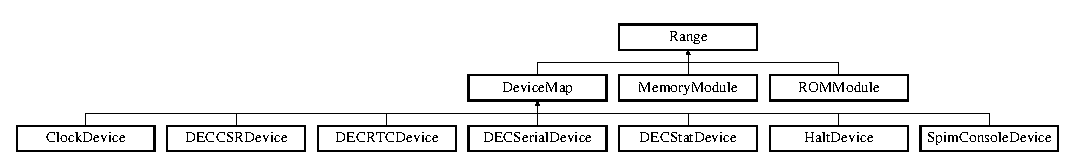
\includegraphics[height=1.80451cm]{classRange}
\end{center}
\end{figure}
\subsection*{Public Member Functions}
\begin{DoxyCompactItemize}
\item 
\hypertarget{classRange_a714d831416094daf2f534435c36b2c8e}{
{\bfseries Range} (uint32 \_\-base, uint32 \_\-extent, caddr\_\-t \_\-address, int \_\-perms)}
\label{classRange_a714d831416094daf2f534435c36b2c8e}

\item 
\hypertarget{classRange_a5076637f68d20251b9800db6a1922ca7}{
virtual bool {\bfseries incorporates} (uint32 addr)  throw ()}
\label{classRange_a5076637f68d20251b9800db6a1922ca7}

\item 
\hypertarget{classRange_a73ad70c479cc77fcf6cb65a8da2993cb}{
virtual bool {\bfseries overlaps} (\hyperlink{classRange}{Range} $\ast$r)  throw ()}
\label{classRange_a73ad70c479cc77fcf6cb65a8da2993cb}

\item 
\hypertarget{classRange_ab4b6e3925cd4559eb8879deed47cb806}{
virtual uint32 {\bfseries getBase} () const }
\label{classRange_ab4b6e3925cd4559eb8879deed47cb806}

\item 
\hypertarget{classRange_addefe753334150b3cbaca2d5f157f17b}{
virtual uint32 {\bfseries getExtent} () const }
\label{classRange_addefe753334150b3cbaca2d5f157f17b}

\item 
\hypertarget{classRange_accb1e300390e551b7b35408413aa99b5}{
virtual void $\ast$ {\bfseries getAddress} () const }
\label{classRange_accb1e300390e551b7b35408413aa99b5}

\item 
\hypertarget{classRange_ac2cb371b9e99eacd063e422b1691204b}{
virtual int {\bfseries getPerms} () const }
\label{classRange_ac2cb371b9e99eacd063e422b1691204b}

\item 
\hypertarget{classRange_a5f60a7e0ad9e6d61d86b82163a78f776}{
virtual void {\bfseries setBase} (uint32 newBase)  throw ()}
\label{classRange_a5f60a7e0ad9e6d61d86b82163a78f776}

\item 
\hypertarget{classRange_a8228499c091dc0eae49f66877a6352c2}{
virtual void {\bfseries setPerms} (int newPerms)  throw ()}
\label{classRange_a8228499c091dc0eae49f66877a6352c2}

\item 
\hypertarget{classRange_a14cad9824900aba8bea2da530e365062}{
virtual bool {\bfseries canRead} (uint32 offset)  throw ()}
\label{classRange_a14cad9824900aba8bea2da530e365062}

\item 
\hypertarget{classRange_aff1be6b26b1c8e4d2b9da3aed0047f61}{
virtual bool {\bfseries canWrite} (uint32 offset)  throw ()}
\label{classRange_aff1be6b26b1c8e4d2b9da3aed0047f61}

\item 
\hypertarget{classRange_a28e79e890739dd67a6c23bf0f7c02af9}{
virtual uint32 {\bfseries fetch\_\-word} (uint32 offset, int mode, \hyperlink{classDeviceExc}{DeviceExc} $\ast$client)}
\label{classRange_a28e79e890739dd67a6c23bf0f7c02af9}

\item 
\hypertarget{classRange_a50db2c6c72990ee650848a1c1fa4fec6}{
virtual uint16 {\bfseries fetch\_\-halfword} (uint32 offset, \hyperlink{classDeviceExc}{DeviceExc} $\ast$client)}
\label{classRange_a50db2c6c72990ee650848a1c1fa4fec6}

\item 
\hypertarget{classRange_af1c0d52a57febea4a3028bdaa09e30f1}{
virtual uint8 {\bfseries fetch\_\-byte} (uint32 offset, \hyperlink{classDeviceExc}{DeviceExc} $\ast$client)}
\label{classRange_af1c0d52a57febea4a3028bdaa09e30f1}

\item 
\hypertarget{classRange_ae39949a0fa25f9496279f8af55ba941a}{
virtual void {\bfseries store\_\-word} (uint32 offset, uint32 data, \hyperlink{classDeviceExc}{DeviceExc} $\ast$client)}
\label{classRange_ae39949a0fa25f9496279f8af55ba941a}

\item 
\hypertarget{classRange_ad2b6650ff9971e2dd21f401008b445ca}{
virtual void {\bfseries store\_\-halfword} (uint32 offset, uint16 data, \hyperlink{classDeviceExc}{DeviceExc} $\ast$client)}
\label{classRange_ad2b6650ff9971e2dd21f401008b445ca}

\item 
\hypertarget{classRange_ac33096c6c3db8aad007facc14f5c0617}{
virtual void {\bfseries store\_\-byte} (uint32 offset, uint8 data, \hyperlink{classDeviceExc}{DeviceExc} $\ast$client)}
\label{classRange_ac33096c6c3db8aad007facc14f5c0617}

\end{DoxyCompactItemize}
\subsection*{Protected Attributes}
\begin{DoxyCompactItemize}
\item 
\hypertarget{classRange_a4086c61cc8ad865a384f469efd86bf65}{
uint32 {\bfseries base}}
\label{classRange_a4086c61cc8ad865a384f469efd86bf65}

\item 
\hypertarget{classRange_a760eb4f06062a8ac89bafc956b2639a2}{
uint32 {\bfseries extent}}
\label{classRange_a760eb4f06062a8ac89bafc956b2639a2}

\item 
\hypertarget{classRange_a6b5d02990f5f9e483e48bcd69047093b}{
void $\ast$ {\bfseries address}}
\label{classRange_a6b5d02990f5f9e483e48bcd69047093b}

\item 
\hypertarget{classRange_a360eeae0c0bdf8b0095c879c9f4cb111}{
int {\bfseries perms}}
\label{classRange_a360eeae0c0bdf8b0095c879c9f4cb111}

\end{DoxyCompactItemize}


The documentation for this class was generated from the following files:\begin{DoxyCompactItemize}
\item 
range.h\item 
range.cc\end{DoxyCompactItemize}

\hypertarget{classProphetStat_1_1RecAdder}{
\section{ProphetStat::RecAdder Class Reference}
\label{classProphetStat_1_1RecAdder}\index{ProphetStat::RecAdder@{ProphetStat::RecAdder}}
}


class \hyperlink{classProphetStat_1_1RecAdder}{RecAdder} wil be inherited by the classes needing statistic to add a \hyperlink{classProphetStat_1_1StatRecord}{StatRecord} instance  




{\ttfamily \#include $<$prophetstatistic.h$>$}

\subsection*{Public Member Functions}
\begin{DoxyCompactItemize}
\item 
\hypertarget{classProphetStat_1_1RecAdder_a2b6cd4108f1c802cc64a7f38e8af00bc}{
\hyperlink{classProphetStat_1_1StatRecord}{StatRecord} $\ast$ {\bfseries GetRec} ()}
\label{classProphetStat_1_1RecAdder_a2b6cd4108f1c802cc64a7f38e8af00bc}

\end{DoxyCompactItemize}
\subsection*{Protected Attributes}
\begin{DoxyCompactItemize}
\item 
\hypertarget{classProphetStat_1_1RecAdder_a5b617fa4c74960bca50be4e7f6a216d6}{
\hyperlink{classProphetStat_1_1StatRecord}{StatRecord} $\ast$ {\bfseries m\_\-Record}}
\label{classProphetStat_1_1RecAdder_a5b617fa4c74960bca50be4e7f6a216d6}

\end{DoxyCompactItemize}


\subsection{Detailed Description}
class \hyperlink{classProphetStat_1_1RecAdder}{RecAdder} wil be inherited by the classes needing statistic to add a \hyperlink{classProphetStat_1_1StatRecord}{StatRecord} instance 

The documentation for this class was generated from the following files:\begin{DoxyCompactItemize}
\item 
prophetstatistic.h\item 
prophetstatistic.cc\end{DoxyCompactItemize}

\hypertarget{structTrace_1_1Record}{
\section{Trace::Record Struct Reference}
\label{structTrace_1_1Record}\index{Trace::Record@{Trace::Record}}
}
\subsection*{Public Types}
\begin{DoxyCompactItemize}
\item 
\hypertarget{structTrace_1_1Record_a180a49f2bfb22355b363e219c964841c}{
typedef std::vector$<$ \hyperlink{structTrace_1_1Operand}{Operand} $>$ {\bfseries OperandListType}}
\label{structTrace_1_1Record_a180a49f2bfb22355b363e219c964841c}

\end{DoxyCompactItemize}
\subsection*{Public Member Functions}
\begin{DoxyCompactItemize}
\item 
\hypertarget{structTrace_1_1Record_ac8273cd7c6aca64757a6dfe5b37d7236}{
void {\bfseries inputs\_\-push\_\-back\_\-op} (const char $\ast$tag, int regno, uint32 val)}
\label{structTrace_1_1Record_ac8273cd7c6aca64757a6dfe5b37d7236}

\item 
\hypertarget{structTrace_1_1Record_a0d4f30b820a0523ab8829a268a0d04ad}{
void {\bfseries inputs\_\-push\_\-back\_\-op} (const char $\ast$tag, uint32 val)}
\label{structTrace_1_1Record_a0d4f30b820a0523ab8829a268a0d04ad}

\item 
\hypertarget{structTrace_1_1Record_a61484ad788baaa57462ebfb23637942d}{
void {\bfseries outputs\_\-push\_\-back\_\-op} (const char $\ast$tag, int regno, uint32 val)}
\label{structTrace_1_1Record_a61484ad788baaa57462ebfb23637942d}

\item 
\hypertarget{structTrace_1_1Record_ac1f177689ea6d50c3bd273b4f930b47f}{
void {\bfseries outputs\_\-push\_\-back\_\-op} (const char $\ast$tag, uint32 val)}
\label{structTrace_1_1Record_ac1f177689ea6d50c3bd273b4f930b47f}

\item 
\hypertarget{structTrace_1_1Record_a795423079fc1202660c2146bd662ebe0}{
void {\bfseries clear} ()}
\label{structTrace_1_1Record_a795423079fc1202660c2146bd662ebe0}

\end{DoxyCompactItemize}
\subsection*{Public Attributes}
\begin{DoxyCompactItemize}
\item 
\hypertarget{structTrace_1_1Record_aba28a18d28949eacc7f9053b6ef85c81}{
OperandListType {\bfseries inputs}}
\label{structTrace_1_1Record_aba28a18d28949eacc7f9053b6ef85c81}

\item 
\hypertarget{structTrace_1_1Record_ae5f156de424fc9289773bca8ecfaff33}{
OperandListType {\bfseries outputs}}
\label{structTrace_1_1Record_ae5f156de424fc9289773bca8ecfaff33}

\item 
\hypertarget{structTrace_1_1Record_a7ef5267ef3122f653c675efd32dbce70}{
uint32 {\bfseries pc}}
\label{structTrace_1_1Record_a7ef5267ef3122f653c675efd32dbce70}

\item 
\hypertarget{structTrace_1_1Record_a78b942443619b45c7484fd22c2274480}{
uint32 {\bfseries instr}}
\label{structTrace_1_1Record_a78b942443619b45c7484fd22c2274480}

\item 
\hypertarget{structTrace_1_1Record_a2412276632ed5e14e36fc75d44fa8bcf}{
uint32 {\bfseries saved\_\-reg} \mbox{[}CPU\_\-REG\_\-NUMBER\mbox{]}}
\label{structTrace_1_1Record_a2412276632ed5e14e36fc75d44fa8bcf}

\end{DoxyCompactItemize}


The documentation for this struct was generated from the following file:\begin{DoxyCompactItemize}
\item 
cpu.h\end{DoxyCompactItemize}

\hypertarget{classPlog_1_1Recorder}{
\section{Plog::Recorder Class Reference}
\label{classPlog_1_1Recorder}\index{Plog::Recorder@{Plog::Recorder}}
}
Inheritance diagram for Plog::Recorder:\begin{figure}[H]
\begin{center}
\leavevmode
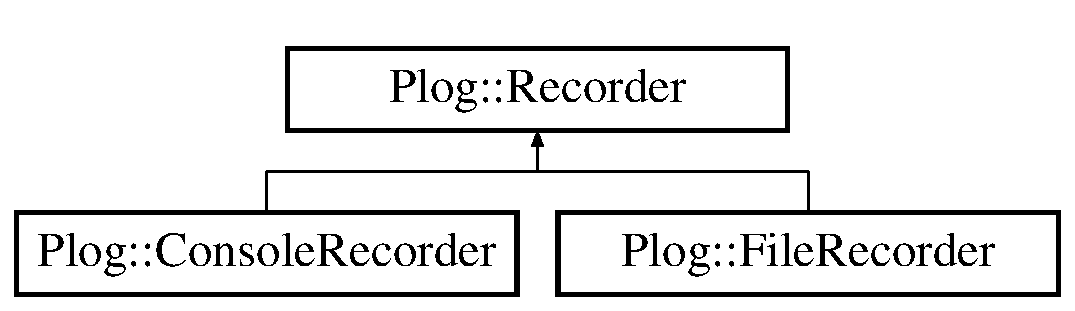
\includegraphics[height=2cm]{classPlog_1_1Recorder}
\end{center}
\end{figure}
\subsection*{Public Member Functions}
\begin{DoxyCompactItemize}
\item 
\hypertarget{classPlog_1_1Recorder_a9c049eccb4393f255881ffa8b80cb98c}{
virtual void {\bfseries RecordMessage} (Plog::PLOG\_\-LEVEL, const std::string \&)=0}
\label{classPlog_1_1Recorder_a9c049eccb4393f255881ffa8b80cb98c}

\item 
\hypertarget{classPlog_1_1Recorder_a6337130ba46fcf60fedb55de9cb5ce96}{
void {\bfseries Enable} (bool work)}
\label{classPlog_1_1Recorder_a6337130ba46fcf60fedb55de9cb5ce96}

\item 
\hypertarget{classPlog_1_1Recorder_a2b75e0a31d40f4376f942e54fef339e5}{
bool {\bfseries IsEnabled} ()}
\label{classPlog_1_1Recorder_a2b75e0a31d40f4376f942e54fef339e5}

\item 
\hypertarget{classPlog_1_1Recorder_a78f446727f7ff5ba803e4a1f3be6a736}{
void {\bfseries WithTime} (bool time)}
\label{classPlog_1_1Recorder_a78f446727f7ff5ba803e4a1f3be6a736}

\item 
\hypertarget{classPlog_1_1Recorder_aa7df41ab647abbef5d74e1130dd0b483}{
bool {\bfseries WantsTime} ()}
\label{classPlog_1_1Recorder_aa7df41ab647abbef5d74e1130dd0b483}

\end{DoxyCompactItemize}


The documentation for this class was generated from the following file:\begin{DoxyCompactItemize}
\item 
prophetlog.cc\end{DoxyCompactItemize}

\hypertarget{classROMModule}{
\section{ROMModule Class Reference}
\label{classROMModule}\index{ROMModule@{ROMModule}}
}
Inheritance diagram for ROMModule:\begin{figure}[H]
\begin{center}
\leavevmode
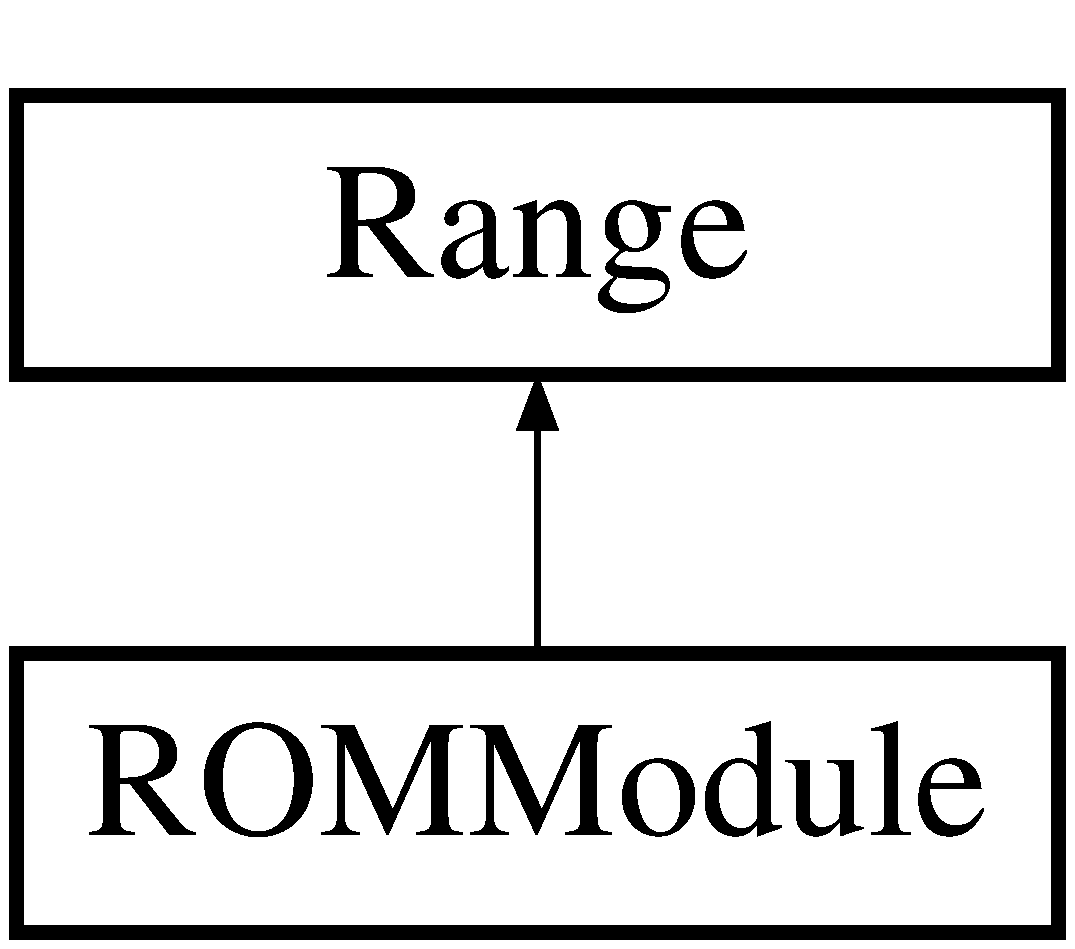
\includegraphics[height=2cm]{classROMModule}
\end{center}
\end{figure}
\subsection*{Public Member Functions}
\begin{DoxyCompactItemize}
\item 
\hypertarget{classROMModule_ad158896a7c2b34808b27b7c6cd37a591}{
{\bfseries ROMModule} (FILE $\ast$f)}
\label{classROMModule_ad158896a7c2b34808b27b7c6cd37a591}

\end{DoxyCompactItemize}


The documentation for this class was generated from the following files:\begin{DoxyCompactItemize}
\item 
rommodule.h\item 
rommodule.cc\end{DoxyCompactItemize}

\hypertarget{classPlog_1_1Setting}{
\section{Plog::Setting Class Reference}
\label{classPlog_1_1Setting}\index{Plog::Setting@{Plog::Setting}}
}
\subsection*{Static Public Member Functions}
\begin{DoxyCompactItemize}
\item 
\hypertarget{classPlog_1_1Setting_a57a98de5300e30c6e7b6116b24844932}{
static \hyperlink{classPlog_1_1Setting}{Setting} $\ast$ {\bfseries Get} ()}
\label{classPlog_1_1Setting_a57a98de5300e30c6e7b6116b24844932}

\end{DoxyCompactItemize}
\subsection*{Public Attributes}
\begin{DoxyCompactItemize}
\item 
\hypertarget{classPlog_1_1Setting_ae780b0802f45be241975826529b4afdc}{
PLOG\_\-LEVEL {\bfseries m\_\-LogLevel}}
\label{classPlog_1_1Setting_ae780b0802f45be241975826529b4afdc}

\item 
\hypertarget{classPlog_1_1Setting_a7ce9f256edbcc73d59b99b7248f3cefa}{
std::string {\bfseries m\_\-File}}
\label{classPlog_1_1Setting_a7ce9f256edbcc73d59b99b7248f3cefa}

\item 
\hypertarget{classPlog_1_1Setting_a2be8c36482b885337070614d6f3f2272}{
bool {\bfseries m\_\-CTime}}
\label{classPlog_1_1Setting_a2be8c36482b885337070614d6f3f2272}

\item 
\hypertarget{classPlog_1_1Setting_addb68862383e97438f322864becc844b}{
bool {\bfseries m\_\-FTime}}
\label{classPlog_1_1Setting_addb68862383e97438f322864becc844b}

\item 
\hypertarget{classPlog_1_1Setting_a50159970f3f4656360ae4fef4ef051ed}{
bool {\bfseries m\_\-EnableConsole}}
\label{classPlog_1_1Setting_a50159970f3f4656360ae4fef4ef051ed}

\item 
\hypertarget{classPlog_1_1Setting_a6b96ec6940210cfd99e90954b376c613}{
bool {\bfseries m\_\-EnableFile}}
\label{classPlog_1_1Setting_a6b96ec6940210cfd99e90954b376c613}

\item 
\hypertarget{classPlog_1_1Setting_ace3bd8c0c1003c63ed9f249d083878bb}{
bool {\bfseries m\_\-PrintLocation}}
\label{classPlog_1_1Setting_ace3bd8c0c1003c63ed9f249d083878bb}

\item 
\hypertarget{classPlog_1_1Setting_aaf06938c4085bb853a6834ef862b5c54}{
Recorders\_\-t {\bfseries m\_\-Recorders}}
\label{classPlog_1_1Setting_aaf06938c4085bb853a6834ef862b5c54}

\item 
\hypertarget{classPlog_1_1Setting_a7976384ea552f28fb0f00f8bcba6816d}{
FatalFunction {\bfseries m\_\-CrashFunction}}
\label{classPlog_1_1Setting_a7976384ea552f28fb0f00f8bcba6816d}

\end{DoxyCompactItemize}


The documentation for this class was generated from the following file:\begin{DoxyCompactItemize}
\item 
prophetlog.cc\end{DoxyCompactItemize}

\hypertarget{structSpawnClientData}{
\section{SpawnClientData Struct Reference}
\label{structSpawnClientData}\index{SpawnClientData@{SpawnClientData}}
}


user defined data passed to its associated actions  




{\ttfamily \#include $<$prophetstatistic.h$>$}

\subsection*{Public Attributes}
\begin{DoxyCompactItemize}
\item 
\hypertarget{structSpawnClientData_a8e35651fe3951d5a6a34ef3dca2e09c6}{
\hyperlink{classProphetStat_1_1RecAdder}{ProphetStat::RecAdder} $\ast$ {\bfseries m\_\-SubAdder}}
\label{structSpawnClientData_a8e35651fe3951d5a6a34ef3dca2e09c6}

\end{DoxyCompactItemize}


\subsection{Detailed Description}
user defined data passed to its associated actions 

The documentation for this struct was generated from the following file:\begin{DoxyCompactItemize}
\item 
prophetstatistic.h\end{DoxyCompactItemize}

\hypertarget{classSpeculativeLogic}{
\section{SpeculativeLogic Class Reference}
\label{classSpeculativeLogic}\index{SpeculativeLogic@{SpeculativeLogic}}
}
\subsection*{Public Types}
\begin{DoxyCompactItemize}
\item 
\hypertarget{classSpeculativeLogic_a2461a666684d4cdcf00181732a8688b3}{
typedef std::list$<$ SpeculativeCPU $\ast$ $>$ {\bfseries SpList}}
\label{classSpeculativeLogic_a2461a666684d4cdcf00181732a8688b3}

\item 
\hypertarget{classSpeculativeLogic_a0f88679e7c8857e42f0d80838ea7cf5c}{
typedef std::list$<$ SpeculativeCPU $\ast$ $>$::iterator {\bfseries SpListIterator}}
\label{classSpeculativeLogic_a0f88679e7c8857e42f0d80838ea7cf5c}

\item 
\hypertarget{classSpeculativeLogic_aa34206026defbc01f2dc57f5a8ff0c67}{
typedef std::list$<$ SpeculativeCPU $\ast$ $>$::const\_\-iterator {\bfseries SpListConstIterator}}
\label{classSpeculativeLogic_aa34206026defbc01f2dc57f5a8ff0c67}

\end{DoxyCompactItemize}
\subsection*{Public Member Functions}
\begin{DoxyCompactItemize}
\item 
\hypertarget{classSpeculativeLogic_acb0f37017ed611ab21c131ed65b21702}{
void {\bfseries SwapToSpList} (SpeculativeCPU $\ast$, SpeculativeCPU $\ast$)}
\label{classSpeculativeLogic_acb0f37017ed611ab21c131ed65b21702}

\item 
\hypertarget{classSpeculativeLogic_a8e5f35ba96b8b0d8f43620550a994529}{
void {\bfseries SwapToFreeList} (SpeculativeCPU $\ast$)}
\label{classSpeculativeLogic_a8e5f35ba96b8b0d8f43620550a994529}

\item 
\hypertarget{classSpeculativeLogic_a84ae57d761581365e019cab467a9b577}{
SpeculativeCPU $\ast$ {\bfseries GetParent} (SpeculativeCPU $\ast$)}
\label{classSpeculativeLogic_a84ae57d761581365e019cab467a9b577}

\item 
\hypertarget{classSpeculativeLogic_a30a3107c14fd7196dc8874ab4177902c}{
SpeculativeCPU $\ast$ {\bfseries GetSubthread} (SpeculativeCPU $\ast$)}
\label{classSpeculativeLogic_a30a3107c14fd7196dc8874ab4177902c}

\item 
\hypertarget{classSpeculativeLogic_a6c5d1030f697921ae4a6dec57c7d9317}{
SpeculativeCPU $\ast$ {\bfseries NotifySpawn} (SpeculativeCPU $\ast$)}
\label{classSpeculativeLogic_a6c5d1030f697921ae4a6dec57c7d9317}

\item 
\hypertarget{classSpeculativeLogic_aa8e34fc7b001120855e0856d9cdd396e}{
void {\bfseries SquashSubthread} (SpeculativeCPU $\ast$, SpeculativeCPU::SQUASH\_\-REASON)}
\label{classSpeculativeLogic_aa8e34fc7b001120855e0856d9cdd396e}

\item 
\hypertarget{classSpeculativeLogic_ae61a5e6d7c9b2fb555396a5ba5aa452b}{
bool {\bfseries VerifySubthread} (SpeculativeCPU $\ast$)}
\label{classSpeculativeLogic_ae61a5e6d7c9b2fb555396a5ba5aa452b}

\item 
\hypertarget{classSpeculativeLogic_aa4eca95eca5abcdeed41287ea6581d09}{
bool {\bfseries PassStableToken} (SpeculativeCPU $\ast$)}
\label{classSpeculativeLogic_aa4eca95eca5abcdeed41287ea6581d09}

\item 
\hypertarget{classSpeculativeLogic_aea27ed6fe3808b6731d3d2e6e9aa1521}{
uint32 {\bfseries GetStackTop} (SpeculativeCPU $\ast$)}
\label{classSpeculativeLogic_aea27ed6fe3808b6731d3d2e6e9aa1521}

\item 
\hypertarget{classSpeculativeLogic_a3b5cfbc29580d96258bff914f8be5f61}{
SpeculativeCPU $\ast$ {\bfseries GetRunner} ()}
\label{classSpeculativeLogic_a3b5cfbc29580d96258bff914f8be5f61}

\item 
\hypertarget{classSpeculativeLogic_a3fd5927ddc4a29f415a016ab38bd6e93}{
void {\bfseries Step} (void)}
\label{classSpeculativeLogic_a3fd5927ddc4a29f415a016ab38bd6e93}

\item 
\hypertarget{classSpeculativeLogic_a6d44073e699460877f7840e4ed7bdaf5}{
void {\bfseries Reset} (void)}
\label{classSpeculativeLogic_a6d44073e699460877f7840e4ed7bdaf5}

\item 
\hypertarget{classSpeculativeLogic_a0e1c5d513f123870ef2722d5b9969d74}{
bool {\bfseries CheckStateOnQuit} ()}
\label{classSpeculativeLogic_a0e1c5d513f123870ef2722d5b9969d74}

\item 
\hypertarget{classSpeculativeLogic_ae8addd001c76eff87101f1c8a3911a23}{
size\_\-t {\bfseries FreeListSize} ()}
\label{classSpeculativeLogic_ae8addd001c76eff87101f1c8a3911a23}

\item 
\hypertarget{classSpeculativeLogic_aefbc24db69f077274b14f607955a7358}{
size\_\-t {\bfseries SpListSize} ()}
\label{classSpeculativeLogic_aefbc24db69f077274b14f607955a7358}

\item 
\hypertarget{classSpeculativeLogic_a0f0e9ab0f1def2f9248b61324f2fc21f}{
int {\bfseries PosInSpList} (SpeculativeCPU $\ast$sender, SpeculativeCPU $\ast$)}
\label{classSpeculativeLogic_a0f0e9ab0f1def2f9248b61324f2fc21f}

\item 
\hypertarget{classSpeculativeLogic_a69fc56353e58b2a63f0711ed2b4831d6}{
int {\bfseries getSpDegree} (SpeculativeCPU $\ast$)}
\label{classSpeculativeLogic_a69fc56353e58b2a63f0711ed2b4831d6}

\end{DoxyCompactItemize}
\subsection*{Static Public Member Functions}
\begin{DoxyCompactItemize}
\item 
\hypertarget{classSpeculativeLogic_af95e558b3c77884f73b10a0fcf480fe5}{
static \hyperlink{classSpeculativeLogic}{SpeculativeLogic} $\ast$ {\bfseries GetInstance} ()}
\label{classSpeculativeLogic_af95e558b3c77884f73b10a0fcf480fe5}

\end{DoxyCompactItemize}


The documentation for this class was generated from the following files:\begin{DoxyCompactItemize}
\item 
speculativelogic.h\item 
speculativelogic.cc\end{DoxyCompactItemize}

\hypertarget{classSpimConsoleDevice}{
\section{SpimConsoleDevice Class Reference}
\label{classSpimConsoleDevice}\index{SpimConsoleDevice@{SpimConsoleDevice}}
}
Inheritance diagram for SpimConsoleDevice:\begin{figure}[H]
\begin{center}
\leavevmode
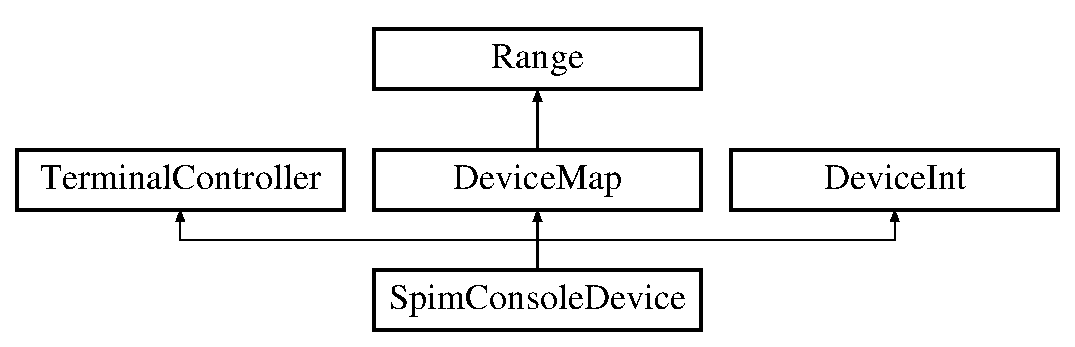
\includegraphics[height=3cm]{classSpimConsoleDevice}
\end{center}
\end{figure}
\subsection*{Classes}
\begin{DoxyCompactItemize}
\item 
class \hyperlink{classSpimConsoleDevice_1_1ClockTrigger}{ClockTrigger}
\end{DoxyCompactItemize}
\subsection*{Public Member Functions}
\begin{DoxyCompactItemize}
\item 
\hypertarget{classSpimConsoleDevice_a5f551a1fb38ddc2fa858e3ba6a7f4d8d}{
{\bfseries SpimConsoleDevice} (\hyperlink{classClock}{Clock} $\ast$clock)  throw ( std::bad\_\-alloc )}
\label{classSpimConsoleDevice_a5f551a1fb38ddc2fa858e3ba6a7f4d8d}

\item 
\hypertarget{classSpimConsoleDevice_a08bf5b3c9651f945ef46fac6f5ab0a8a}{
virtual void {\bfseries ready\_\-display} (int line)  throw ()}
\label{classSpimConsoleDevice_a08bf5b3c9651f945ef46fac6f5ab0a8a}

\item 
\hypertarget{classSpimConsoleDevice_a05eaad591781ef58baad9905c2f3dbde}{
virtual void {\bfseries unready\_\-display} (int line, char data)  throw ( std::bad\_\-alloc )}
\label{classSpimConsoleDevice_a05eaad591781ef58baad9905c2f3dbde}

\item 
\hypertarget{classSpimConsoleDevice_a69b27e3320892b3190c94bc0124c3705}{
virtual void {\bfseries unready\_\-keyboard} (int line)  throw ()}
\label{classSpimConsoleDevice_a69b27e3320892b3190c94bc0124c3705}

\item 
\hypertarget{classSpimConsoleDevice_a4a6473276fdd22bb253b0275d3aaf622}{
virtual void {\bfseries ready\_\-clock} ()  throw ( std::bad\_\-alloc )}
\label{classSpimConsoleDevice_a4a6473276fdd22bb253b0275d3aaf622}

\item 
\hypertarget{classSpimConsoleDevice_a3feff73864a3fc39e88924c2ae29b358}{
virtual void {\bfseries unready\_\-clock} ()  throw ()}
\label{classSpimConsoleDevice_a3feff73864a3fc39e88924c2ae29b358}

\item 
\hypertarget{classSpimConsoleDevice_a10a8f062fcee183b49c1cfaab2d729cb}{
virtual uint32 {\bfseries fetch\_\-word} (uint32 offset, int mode, \hyperlink{classDeviceExc}{DeviceExc} $\ast$client)}
\label{classSpimConsoleDevice_a10a8f062fcee183b49c1cfaab2d729cb}

\item 
\hypertarget{classSpimConsoleDevice_a171e1c405553688ac6d7a344579c4762}{
virtual void {\bfseries store\_\-word} (uint32 offset, uint32 data, \hyperlink{classDeviceExc}{DeviceExc} $\ast$client)}
\label{classSpimConsoleDevice_a171e1c405553688ac6d7a344579c4762}

\item 
\hypertarget{classSpimConsoleDevice_ade305bc5e335fc57fde48661b2fac932}{
virtual const char $\ast$ {\bfseries descriptor\_\-str} () const }
\label{classSpimConsoleDevice_ade305bc5e335fc57fde48661b2fac932}

\end{DoxyCompactItemize}
\subsection*{Protected Member Functions}
\begin{DoxyCompactItemize}
\item 
\hypertarget{classSpimConsoleDevice_a1d4e7b7cf74058b78b97c1b38989fb32}{
virtual void {\bfseries ready\_\-keyboard} (int line)  throw ()}
\label{classSpimConsoleDevice_a1d4e7b7cf74058b78b97c1b38989fb32}

\end{DoxyCompactItemize}
\subsection*{Protected Attributes}
\begin{DoxyCompactItemize}
\item 
\hypertarget{classSpimConsoleDevice_a9d198eda9fea1f785d1e1a5b6dee989f}{
\hyperlink{classSpimConsoleDevice_1_1ClockTrigger}{ClockTrigger} $\ast$ {\bfseries trigger}}
\label{classSpimConsoleDevice_a9d198eda9fea1f785d1e1a5b6dee989f}

\item 
\hypertarget{classSpimConsoleDevice_a4f18e808134f6316b56414af76ef5166}{
bool {\bfseries display\_\-interrupt\_\-enable} \mbox{[}2\mbox{]}}
\label{classSpimConsoleDevice_a4f18e808134f6316b56414af76ef5166}

\item 
\hypertarget{classSpimConsoleDevice_ac630afbba920b08a99d58abac7ee8db0}{
bool {\bfseries keyboard\_\-interrupt\_\-enable} \mbox{[}2\mbox{]}}
\label{classSpimConsoleDevice_ac630afbba920b08a99d58abac7ee8db0}

\item 
\hypertarget{classSpimConsoleDevice_ad7800f8b1f3f8901eb442ec9b43e4d44}{
bool {\bfseries clock\_\-interrupt}}
\label{classSpimConsoleDevice_ad7800f8b1f3f8901eb442ec9b43e4d44}

\item 
\hypertarget{classSpimConsoleDevice_a1151ad9401979e409f63d3ce3cb2747f}{
State {\bfseries clock\_\-state}}
\label{classSpimConsoleDevice_a1151ad9401979e409f63d3ce3cb2747f}

\end{DoxyCompactItemize}
\subsection*{Static Protected Attributes}
\begin{DoxyCompactItemize}
\item 
\hypertarget{classSpimConsoleDevice_a4f5c6639fafcb0e60141c55d42e74c80}{
static const long {\bfseries KEYBOARD\_\-POLL\_\-NS} = 400 $\ast$ 1000}
\label{classSpimConsoleDevice_a4f5c6639fafcb0e60141c55d42e74c80}

\item 
\hypertarget{classSpimConsoleDevice_a42c7c6cd43f403cbfaf11e4e688145e3}{
static const long {\bfseries KEYBOARD\_\-REPOLL\_\-NS} = 40 $\ast$ 1000 $\ast$ 1000}
\label{classSpimConsoleDevice_a42c7c6cd43f403cbfaf11e4e688145e3}

\item 
\hypertarget{classSpimConsoleDevice_a63a0316380e0fec7d91e01fb41e962af}{
static const long {\bfseries DISPLAY\_\-READY\_\-DELAY\_\-NS} = 40 $\ast$ 1000 $\ast$ 1000}
\label{classSpimConsoleDevice_a63a0316380e0fec7d91e01fb41e962af}

\item 
\hypertarget{classSpimConsoleDevice_a6ee877243858bff6624f76b87db50320}{
static const long {\bfseries CLOCK\_\-TRIGGER\_\-NS} = 1000 $\ast$ 1000 $\ast$1000}
\label{classSpimConsoleDevice_a6ee877243858bff6624f76b87db50320}

\end{DoxyCompactItemize}


The documentation for this class was generated from the following files:\begin{DoxyCompactItemize}
\item 
spimconsole.h\item 
spimconsole.cc\end{DoxyCompactItemize}

\hypertarget{structSquashClientData}{
\section{SquashClientData Struct Reference}
\label{structSquashClientData}\index{SquashClientData@{SquashClientData}}
}
\subsection*{Public Attributes}
\begin{DoxyCompactItemize}
\item 
\hypertarget{structSquashClientData_a02d8bd7ce5dcbdecc42d2286c5f4d792}{
const char $\ast$ {\bfseries m\_\-Reason}}
\label{structSquashClientData_a02d8bd7ce5dcbdecc42d2286c5f4d792}

\item 
\hypertarget{structSquashClientData_a6203a9812d96721ec44613d996977cdf}{
int {\bfseries m\_\-DisInSpList}}
\label{structSquashClientData_a6203a9812d96721ec44613d996977cdf}

\end{DoxyCompactItemize}


The documentation for this struct was generated from the following file:\begin{DoxyCompactItemize}
\item 
prophetstatistic.h\end{DoxyCompactItemize}

\hypertarget{classProphetStat_1_1SquashOnSpList}{
\section{ProphetStat::SquashOnSpList Class Reference}
\label{classProphetStat_1_1SquashOnSpList}\index{ProphetStat::SquashOnSpList@{ProphetStat::SquashOnSpList}}
}
\subsection*{Public Member Functions}
\begin{DoxyCompactItemize}
\item 
\hypertarget{classProphetStat_1_1SquashOnSpList_a83814cf7d6a2590cdf55d7ba913f6aab}{
void {\bfseries addToList} (SquashOrSpawn state, int posSpList)}
\label{classProphetStat_1_1SquashOnSpList_a83814cf7d6a2590cdf55d7ba913f6aab}

\item 
\hypertarget{classProphetStat_1_1SquashOnSpList_a94b56064cbc458c271b2494bb437b082}{
void {\bfseries addToXml} (\hyperlink{classXmlElement}{XmlElement} $\ast$root)}
\label{classProphetStat_1_1SquashOnSpList_a94b56064cbc458c271b2494bb437b082}

\item 
\hypertarget{classProphetStat_1_1SquashOnSpList_a4bffc14013536873a62dd0f98d4d69e8}{
void {\bfseries printList} (FILE $\ast$fp=stderr)}
\label{classProphetStat_1_1SquashOnSpList_a4bffc14013536873a62dd0f98d4d69e8}

\item 
\hypertarget{classProphetStat_1_1SquashOnSpList_aceea97fb1e7f46c34fa46fecbfdb7922}{
void {\bfseries calProp} ()}
\label{classProphetStat_1_1SquashOnSpList_aceea97fb1e7f46c34fa46fecbfdb7922}

\end{DoxyCompactItemize}
\subsection*{Static Public Member Functions}
\begin{DoxyCompactItemize}
\item 
\hypertarget{classProphetStat_1_1SquashOnSpList_a7ab26166ecb4d874d08b565c287e7124}{
static \hyperlink{classProphetStat_1_1SquashOnSpList}{SquashOnSpList} $\ast$ {\bfseries getInstance} (int num)}
\label{classProphetStat_1_1SquashOnSpList_a7ab26166ecb4d874d08b565c287e7124}

\end{DoxyCompactItemize}


The documentation for this class was generated from the following files:\begin{DoxyCompactItemize}
\item 
prophetcpustat.h\item 
prophetcpustat.cc\end{DoxyCompactItemize}

\hypertarget{structProphetStat_1_1StatCpu}{
\section{ProphetStat::StatCpu Struct Reference}
\label{structProphetStat_1_1StatCpu}\index{ProphetStat::StatCpu@{ProphetStat::StatCpu}}
}


{\ttfamily \#include $<$prophetstatistic.h$>$}

\subsection*{Public Member Functions}
\begin{DoxyCompactItemize}
\item 
\hypertarget{structProphetStat_1_1StatCpu_a6e4ce4ed546daef76b87825bc2b4a52c}{
double {\bfseries averageCoreNum} ()}
\label{structProphetStat_1_1StatCpu_a6e4ce4ed546daef76b87825bc2b4a52c}

\item 
\hypertarget{structProphetStat_1_1StatCpu_a9fba1d4e54315792e05bc32ff3908e6e}{
double $\ast$ {\bfseries calProportion} ()}
\label{structProphetStat_1_1StatCpu_a9fba1d4e54315792e05bc32ff3908e6e}

\end{DoxyCompactItemize}
\subsection*{Static Public Member Functions}
\begin{DoxyCompactItemize}
\item 
\hypertarget{structProphetStat_1_1StatCpu_a8bcebe874f1f2281914831c2f29e7b94}{
static \hyperlink{structProphetStat_1_1StatCpu}{StatCpu} $\ast$ {\bfseries getStatCpuInstance} (int n)}
\label{structProphetStat_1_1StatCpu_a8bcebe874f1f2281914831c2f29e7b94}

\end{DoxyCompactItemize}
\subsection*{Public Attributes}
\begin{DoxyCompactItemize}
\item 
\hypertarget{structProphetStat_1_1StatCpu_a17060d381054d9f4cfde5e45a1a68801}{
int {\bfseries num}}
\label{structProphetStat_1_1StatCpu_a17060d381054d9f4cfde5e45a1a68801}

\item 
\hypertarget{structProphetStat_1_1StatCpu_a0ce6afabe767f77c09c722ee0ed2f5f2}{
int $\ast$ {\bfseries coreNum}}
\label{structProphetStat_1_1StatCpu_a0ce6afabe767f77c09c722ee0ed2f5f2}

\item 
\hypertarget{structProphetStat_1_1StatCpu_a5d8ad59ddc734b1bb5df2bb9340ff045}{
double $\ast$ {\bfseries proportion}}
\label{structProphetStat_1_1StatCpu_a5d8ad59ddc734b1bb5df2bb9340ff045}

\end{DoxyCompactItemize}
\subsection*{Static Public Attributes}
\begin{DoxyCompactItemize}
\item 
\hypertarget{structProphetStat_1_1StatCpu_a23a77b4ddaf86f71fe1c4aed534ff303}{
static \hyperlink{structProphetStat_1_1StatCpu}{StatCpu} $\ast$ {\bfseries hasone} = NULL}
\label{structProphetStat_1_1StatCpu_a23a77b4ddaf86f71fe1c4aed534ff303}

\end{DoxyCompactItemize}


\subsection{Detailed Description}
统计CPU核利用率, 主要从在某一时刻, 有多少个核在同时运行这个方面进行统计的。 这个是单例模式, 使用getStatCpuInstance来构造一个唯一的对象。 

The documentation for this struct was generated from the following files:\begin{DoxyCompactItemize}
\item 
prophetstatistic.h\item 
prophetstatistic.cc\end{DoxyCompactItemize}

\hypertarget{classProphetStat_1_1Statistic}{
\section{ProphetStat::Statistic Class Reference}
\label{classProphetStat_1_1Statistic}\index{ProphetStat::Statistic@{ProphetStat::Statistic}}
}


\hyperlink{classProphetStat_1_1Statistic}{Statistic} maintains all the statistic record for the cpus.  


\subsection*{Public Member Functions}
\begin{DoxyCompactItemize}
\item 
\hypertarget{classProphetStat_1_1Statistic_aaaf8c7d24fec7daaa91ae86cf34df8e7}{
void {\bfseries RegisterRec} (\hyperlink{classProphetStat_1_1StatRecord}{StatRecord} $\ast$)}
\label{classProphetStat_1_1Statistic_aaaf8c7d24fec7daaa91ae86cf34df8e7}

\item 
\hypertarget{classProphetStat_1_1Statistic_a97156929bf7aea0054539e2ee14ce6ed}{
\hyperlink{classXmlElement}{XmlElement} $\ast$ {\bfseries AddToXml} (\hyperlink{classXmlElement}{XmlElement} $\ast$)}
\label{classProphetStat_1_1Statistic_a97156929bf7aea0054539e2ee14ce6ed}

\item 
\hypertarget{classProphetStat_1_1Statistic_a42df9e3d53fa6f1097662d2b2162f4f9}{
\hyperlink{classXmlElement}{XmlElement} $\ast$ {\bfseries AddStat} (\hyperlink{classXmlElement}{XmlElement} $\ast$)}
\label{classProphetStat_1_1Statistic_a42df9e3d53fa6f1097662d2b2162f4f9}

\end{DoxyCompactItemize}
\subsection*{Static Public Member Functions}
\begin{DoxyCompactItemize}
\item 
\hypertarget{classProphetStat_1_1Statistic_a20d8045bf9fa6c491d58c810c7bcfdf1}{
static \hyperlink{classProphetStat_1_1Statistic}{Statistic} $\ast$ {\bfseries Get} ()}
\label{classProphetStat_1_1Statistic_a20d8045bf9fa6c491d58c810c7bcfdf1}

\end{DoxyCompactItemize}


\subsection{Detailed Description}
\hyperlink{classProphetStat_1_1Statistic}{Statistic} maintains all the statistic record for the cpus. 

The documentation for this class was generated from the following file:\begin{DoxyCompactItemize}
\item 
prophetstatistic.cc\end{DoxyCompactItemize}

\hypertarget{structProphetStat_1_1StatItem}{
\section{ProphetStat::StatItem Struct Reference}
\label{structProphetStat_1_1StatItem}\index{ProphetStat::StatItem@{ProphetStat::StatItem}}
}


instruction hash list item, its content is loaded from setting file  




{\ttfamily \#include $<$prophetstatistic.h$>$}

\subsection*{Public Attributes}
\begin{DoxyCompactItemize}
\item 
\hypertarget{structProphetStat_1_1StatItem_a5ccca91275abbbf583d84417d1334dfe}{
int {\bfseries m\_\-Cost}}
\label{structProphetStat_1_1StatItem_a5ccca91275abbbf583d84417d1334dfe}

\item 
\hypertarget{structProphetStat_1_1StatItem_aaccb4e5101e8fbe1ccbe634abc7dea8a}{
STAT\_\-ACTION {\bfseries m\_\-Action}}
\label{structProphetStat_1_1StatItem_aaccb4e5101e8fbe1ccbe634abc7dea8a}

\end{DoxyCompactItemize}


\subsection{Detailed Description}
instruction hash list item, its content is loaded from setting file 

The documentation for this struct was generated from the following file:\begin{DoxyCompactItemize}
\item 
prophetstatistic.h\end{DoxyCompactItemize}

\hypertarget{classProphetStat_1_1StatRecord}{
\section{ProphetStat::StatRecord Class Reference}
\label{classProphetStat_1_1StatRecord}\index{ProphetStat::StatRecord@{ProphetStat::StatRecord}}
}


a class to store the statistical variables  




{\ttfamily \#include $<$prophetstatistic.h$>$}

\subsection*{Public Member Functions}
\begin{DoxyCompactItemize}
\item 
\hypertarget{classProphetStat_1_1StatRecord_a416ba4e0c158e1b767d8aa2ed9e641f7}{
\hyperlink{classXmlElement}{XmlElement} $\ast$ {\bfseries XmlNode} ()}
\label{classProphetStat_1_1StatRecord_a416ba4e0c158e1b767d8aa2ed9e641f7}

\end{DoxyCompactItemize}
\subsection*{Public Attributes}
\begin{DoxyCompactItemize}
\item 
\hypertarget{classProphetStat_1_1StatRecord_adcaf3b295803c9b7465e36d65a65cd2f}{
int {\bfseries m\_\-TotalInst}}
\label{classProphetStat_1_1StatRecord_adcaf3b295803c9b7465e36d65a65cd2f}

\item 
\hypertarget{classProphetStat_1_1StatRecord_a6089b42fc0f5f237e29c816c3cf04fb5}{
int {\bfseries m\_\-TotalClock}}
\label{classProphetStat_1_1StatRecord_a6089b42fc0f5f237e29c816c3cf04fb5}

\item 
\hypertarget{classProphetStat_1_1StatRecord_a80f35b54d4f3d71ec1adbe1fc8d1c8d7}{
int {\bfseries m\_\-SpawnedThread}}
\label{classProphetStat_1_1StatRecord_a80f35b54d4f3d71ec1adbe1fc8d1c8d7}

\item 
\hypertarget{classProphetStat_1_1StatRecord_a675632b8cdb330e399fafee02d28d91f}{
int {\bfseries m\_\-CommitedThread}}
\label{classProphetStat_1_1StatRecord_a675632b8cdb330e399fafee02d28d91f}

\item 
\hypertarget{classProphetStat_1_1StatRecord_a85a86c8f03bb2639d3632d938dce1623}{
int {\bfseries m\_\-FailedThread}}
\label{classProphetStat_1_1StatRecord_a85a86c8f03bb2639d3632d938dce1623}

\item 
\hypertarget{classProphetStat_1_1StatRecord_a9c9d065b110c636a5c0a33ff778a32ab}{
int {\bfseries m\_\-FailOnDDV}}
\label{classProphetStat_1_1StatRecord_a9c9d065b110c636a5c0a33ff778a32ab}

\item 
\hypertarget{classProphetStat_1_1StatRecord_a6eb48e8025ddbaf03c9821ecf0ece141}{
int {\bfseries m\_\-FailOnInstruction}}
\label{classProphetStat_1_1StatRecord_a6eb48e8025ddbaf03c9821ecf0ece141}

\item 
\hypertarget{classProphetStat_1_1StatRecord_a0d56f4c698ccb4be2cc53a26472299d2}{
int {\bfseries m\_\-FailOnRegV}}
\label{classProphetStat_1_1StatRecord_a0d56f4c698ccb4be2cc53a26472299d2}

\item 
\hypertarget{classProphetStat_1_1StatRecord_affe6402022a08df397f6d116d05da17f}{
int {\bfseries m\_\-FailOnMMV}}
\label{classProphetStat_1_1StatRecord_affe6402022a08df397f6d116d05da17f}

\item 
\hypertarget{classProphetStat_1_1StatRecord_a6592e18e0a97cc20ac56d0b6cc2c65de}{
int {\bfseries m\_\-FailOnLowPriority}}
\label{classProphetStat_1_1StatRecord_a6592e18e0a97cc20ac56d0b6cc2c65de}

\item 
\hypertarget{classProphetStat_1_1StatRecord_a18420ad96ce376d50f64ae8d24cf25b8}{
int {\bfseries m\_\-FailOnControl}}
\label{classProphetStat_1_1StatRecord_a18420ad96ce376d50f64ae8d24cf25b8}

\item 
\hypertarget{classProphetStat_1_1StatRecord_a2b66d08cc571964ed5fd7f6c75decacb}{
int {\bfseries m\_\-FailOnReset}}
\label{classProphetStat_1_1StatRecord_a2b66d08cc571964ed5fd7f6c75decacb}

\item 
\hypertarget{classProphetStat_1_1StatRecord_aa720c4c24423432491a2d3dd4625d3a6}{
int {\bfseries m\_\-FailOnHalt}}
\label{classProphetStat_1_1StatRecord_aa720c4c24423432491a2d3dd4625d3a6}

\item 
\hypertarget{classProphetStat_1_1StatRecord_a3131a4ce6e94b8b6b373320ee9597cf7}{
int {\bfseries m\_\-FailOnQuit}}
\label{classProphetStat_1_1StatRecord_a3131a4ce6e94b8b6b373320ee9597cf7}

\item 
\hypertarget{classProphetStat_1_1StatRecord_a6c8918e48850d149777aa13c2c409d82}{
int {\bfseries m\_\-FailOnException}}
\label{classProphetStat_1_1StatRecord_a6c8918e48850d149777aa13c2c409d82}

\item 
\hypertarget{classProphetStat_1_1StatRecord_acf575606eca1e925b2031331414f8c51}{
int {\bfseries m\_\-FailOnUnknown}}
\label{classProphetStat_1_1StatRecord_acf575606eca1e925b2031331414f8c51}

\item 
\hypertarget{classProphetStat_1_1StatRecord_ac75ae7acd227a411c409a15db51c964f}{
int {\bfseries m\_\-StartTime}}
\label{classProphetStat_1_1StatRecord_ac75ae7acd227a411c409a15db51c964f}

\item 
\hypertarget{classProphetStat_1_1StatRecord_a836ee85204d65d771ca87c6da8260a83}{
int {\bfseries m\_\-FinishTime}}
\label{classProphetStat_1_1StatRecord_a836ee85204d65d771ca87c6da8260a83}

\item 
\hypertarget{classProphetStat_1_1StatRecord_ae2b0d2cbb93d739409c78b729880bbd8}{
int $\ast$ {\bfseries m\_\-FailNumBuf}}
\label{classProphetStat_1_1StatRecord_ae2b0d2cbb93d739409c78b729880bbd8}

\item 
\hypertarget{classProphetStat_1_1StatRecord_a63c9ad764eea13134f90185c6dcdfa7f}{
\hyperlink{structProphetStat_1_1StatTime}{StatTime} $\ast$ {\bfseries m\_\-TimeStatistic}}
\label{classProphetStat_1_1StatRecord_a63c9ad764eea13134f90185c6dcdfa7f}

\end{DoxyCompactItemize}
\subsection*{Static Public Attributes}
\begin{DoxyCompactItemize}
\item 
\hypertarget{classProphetStat_1_1StatRecord_a2002cb849842096dd9724a5948a9fef3}{
static int {\bfseries m\_\-FailNumBufSize} = 0}
\label{classProphetStat_1_1StatRecord_a2002cb849842096dd9724a5948a9fef3}

\item 
\hypertarget{classProphetStat_1_1StatRecord_a877704fda335e3067af262a2b2e41e44}{
static \hyperlink{structProphetStat_1_1StatCpu}{StatCpu} $\ast$ {\bfseries m\_\-CpuStat} = NULL}
\label{classProphetStat_1_1StatRecord_a877704fda335e3067af262a2b2e41e44}

\item 
\hypertarget{classProphetStat_1_1StatRecord_a7ddc6930036810c1b24addc59f9cc0a4}{
static int {\bfseries m\_\-SeqTime} = 0}
\label{classProphetStat_1_1StatRecord_a7ddc6930036810c1b24addc59f9cc0a4}

\item 
\hypertarget{classProphetStat_1_1StatRecord_ab74d5acea0265b52037090c4c5e9416a}{
static int {\bfseries m\_\-ParalTime} = 0}
\label{classProphetStat_1_1StatRecord_ab74d5acea0265b52037090c4c5e9416a}

\item 
\hypertarget{classProphetStat_1_1StatRecord_a5ced35d9aadf20c7026fb0279fa36fd1}{
static int {\bfseries m\_\-ClockParalTime} = 0}
\label{classProphetStat_1_1StatRecord_a5ced35d9aadf20c7026fb0279fa36fd1}

\end{DoxyCompactItemize}


\subsection{Detailed Description}
a class to store the statistical variables 非静态属性 只统计单个核(由单个对象表示)上的若干参数, 静态属性统计全局的(所有对象,所有核上)参数 因此非静态属性使用时, 最后要把所有的核统计的结果累加, 而静态属性不需要累加 

The documentation for this class was generated from the following files:\begin{DoxyCompactItemize}
\item 
prophetstatistic.h\item 
prophetstatistic.cc\end{DoxyCompactItemize}

\hypertarget{structProphetStat_1_1StatTime}{
\section{ProphetStat::StatTime Struct Reference}
\label{structProphetStat_1_1StatTime}\index{ProphetStat::StatTime@{ProphetStat::StatTime}}
}
\subsection*{Public Member Functions}
\begin{DoxyCompactItemize}
\item 
\hypertarget{structProphetStat_1_1StatTime_a78dd2e2fb84673db1d28f210e1830257}{
long {\bfseries setTotalTime} ()}
\label{structProphetStat_1_1StatTime_a78dd2e2fb84673db1d28f210e1830257}

\end{DoxyCompactItemize}
\subsection*{Public Attributes}
\begin{DoxyCompactItemize}
\item 
\hypertarget{structProphetStat_1_1StatTime_ac676df9157635eaffc5bd02f654daee9}{
int {\bfseries m\_\-freeTime}}
\label{structProphetStat_1_1StatTime_ac676df9157635eaffc5bd02f654daee9}

\item 
\hypertarget{structProphetStat_1_1StatTime_aa3ec64ca05e740139b76184158169db0}{
int {\bfseries m\_\-squashTime}}
\label{structProphetStat_1_1StatTime_aa3ec64ca05e740139b76184158169db0}

\item 
\hypertarget{structProphetStat_1_1StatTime_ae7ddad00f7aaeb89b70c155a240ff2c9}{
int {\bfseries m\_\-waitTime}}
\label{structProphetStat_1_1StatTime_ae7ddad00f7aaeb89b70c155a240ff2c9}

\item 
\hypertarget{structProphetStat_1_1StatTime_a594256279592f8f1776ecb4191322657}{
int {\bfseries m\_\-spTime}}
\label{structProphetStat_1_1StatTime_a594256279592f8f1776ecb4191322657}

\item 
\hypertarget{structProphetStat_1_1StatTime_a930e8175516047464f9eb041173bd210}{
int {\bfseries m\_\-noSptime}}
\label{structProphetStat_1_1StatTime_a930e8175516047464f9eb041173bd210}

\item 
\hypertarget{structProphetStat_1_1StatTime_a645cbfe1814ac1af3a4644573998b210}{
int {\bfseries m\_\-timeSlot}}
\label{structProphetStat_1_1StatTime_a645cbfe1814ac1af3a4644573998b210}

\item 
\hypertarget{structProphetStat_1_1StatTime_ac9887a51cf8fc6875cc2e8a7c8b587ce}{
int {\bfseries m\_\-timeNeedVerify}}
\label{structProphetStat_1_1StatTime_ac9887a51cf8fc6875cc2e8a7c8b587ce}

\item 
\hypertarget{structProphetStat_1_1StatTime_a3bfe4024fcde7a64c301355abc74f400}{
long {\bfseries m\_\-totalTime}}
\label{structProphetStat_1_1StatTime_a3bfe4024fcde7a64c301355abc74f400}

\item 
\hypertarget{structProphetStat_1_1StatTime_a3fde3247b4aae233cf4af8d18b1cb0e3}{
int {\bfseries m\_\-psliceTime}}
\label{structProphetStat_1_1StatTime_a3fde3247b4aae233cf4af8d18b1cb0e3}

\item 
\hypertarget{structProphetStat_1_1StatTime_a28277280c2a3516ec0e9bb496846356d}{
int {\bfseries m\_\-lastFinishTime}}
\label{structProphetStat_1_1StatTime_a28277280c2a3516ec0e9bb496846356d}

\item 
\hypertarget{structProphetStat_1_1StatTime_a9e1958fda986447845cb2da7d9c575ea}{
StatState {\bfseries m\_\-runState}}
\label{structProphetStat_1_1StatTime_a9e1958fda986447845cb2da7d9c575ea}

\end{DoxyCompactItemize}


The documentation for this struct was generated from the following files:\begin{DoxyCompactItemize}
\item 
prophetstatistic.h\item 
prophetstatistic.cc\end{DoxyCompactItemize}

\hypertarget{classTask}{
\section{Task Class Reference}
\label{classTask}\index{Task@{Task}}
}
Inheritance diagram for Task:\begin{figure}[H]
\begin{center}
\leavevmode
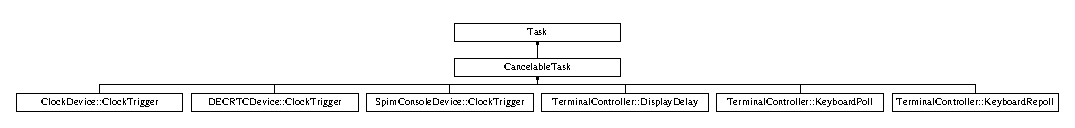
\includegraphics[height=1.27273cm]{classTask}
\end{center}
\end{figure}
\subsection*{Public Member Functions}
\begin{DoxyCompactItemize}
\item 
\hypertarget{classTask_a87488fcdd09c9a0200913333fb6c9c32}{
virtual void {\bfseries task} ()=0}
\label{classTask_a87488fcdd09c9a0200913333fb6c9c32}

\end{DoxyCompactItemize}


The documentation for this class was generated from the following file:\begin{DoxyCompactItemize}
\item 
task.h\end{DoxyCompactItemize}

\hypertarget{classTerminalController}{
\section{TerminalController Class Reference}
\label{classTerminalController}\index{TerminalController@{TerminalController}}
}
Inheritance diagram for TerminalController:\begin{figure}[H]
\begin{center}
\leavevmode
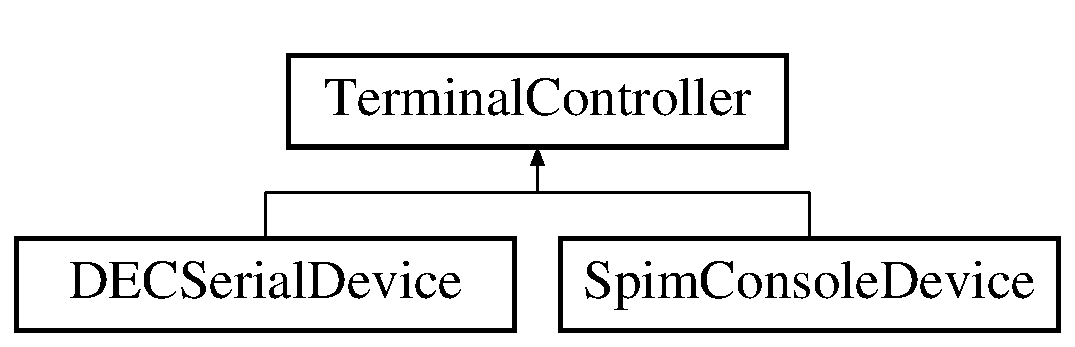
\includegraphics[height=2cm]{classTerminalController}
\end{center}
\end{figure}
\subsection*{Classes}
\begin{DoxyCompactItemize}
\item 
class \hyperlink{classTerminalController_1_1DisplayDelay}{DisplayDelay}
\item 
class \hyperlink{classTerminalController_1_1KeyboardPoll}{KeyboardPoll}
\item 
class \hyperlink{classTerminalController_1_1KeyboardRepoll}{KeyboardRepoll}
\item 
struct \hyperlink{structTerminalController_1_1LineState}{LineState}
\end{DoxyCompactItemize}
\subsection*{Public Member Functions}
\begin{DoxyCompactItemize}
\item 
\hypertarget{classTerminalController_a1c0eb6e303af08fd8a3339f148947d45}{
{\bfseries TerminalController} (\hyperlink{classClock}{Clock} $\ast$clock, long keyboard\_\-poll\_\-ns, long keyboard\_\-repoll\_\-ns, long display\_\-ready\_\-delay\_\-ns)  throw ( std::bad\_\-alloc )}
\label{classTerminalController_a1c0eb6e303af08fd8a3339f148947d45}

\item 
\hypertarget{classTerminalController_acf0828324151635cac47807c736a1308}{
virtual bool {\bfseries connect\_\-terminal} (int tty\_\-fd, int line)  throw ()}
\label{classTerminalController_acf0828324151635cac47807c736a1308}

\item 
\hypertarget{classTerminalController_aea2409c72052fcd47289b447f83eb10a}{
virtual void {\bfseries remove\_\-terminal} (int line)  throw ()}
\label{classTerminalController_aea2409c72052fcd47289b447f83eb10a}

\item 
\hypertarget{classTerminalController_a157b1f7b289043c3b27470230875d9c3}{
bool {\bfseries line\_\-connected} (const int line) const }
\label{classTerminalController_a157b1f7b289043c3b27470230875d9c3}

\item 
\hypertarget{classTerminalController_a0e2d66f0e2cbe7373bf8e0ba4ac6c5b1}{
virtual void {\bfseries reinitialize\_\-terminals} ()  throw ()}
\label{classTerminalController_a0e2d66f0e2cbe7373bf8e0ba4ac6c5b1}

\item 
\hypertarget{classTerminalController_a343a40e774eeb2506b0bfbc5817d0c62}{
virtual void {\bfseries poll\_\-keyboards} ()  throw ( std::bad\_\-alloc )}
\label{classTerminalController_a343a40e774eeb2506b0bfbc5817d0c62}

\item 
\hypertarget{classTerminalController_a985b6892fc255a919238acecb947a978}{
virtual void {\bfseries repoll\_\-keyboard} (int line)  throw ( std::bad\_\-alloc )}
\label{classTerminalController_a985b6892fc255a919238acecb947a978}

\item 
\hypertarget{classTerminalController_acf0314b08dad27cfe57bf374cecbc5a3}{
virtual void {\bfseries unready\_\-display} (int line, char data)  throw ( std::bad\_\-alloc )}
\label{classTerminalController_acf0314b08dad27cfe57bf374cecbc5a3}

\item 
\hypertarget{classTerminalController_a38a988039e7bcb29a7b6b74273d99ffa}{
virtual void {\bfseries ready\_\-display} (int line)  throw ()}
\label{classTerminalController_a38a988039e7bcb29a7b6b74273d99ffa}

\item 
\hypertarget{classTerminalController_afe5b8685b5149db2b7cc5b2e395a479e}{
virtual void {\bfseries unready\_\-keyboard} (int line)  throw ()}
\label{classTerminalController_afe5b8685b5149db2b7cc5b2e395a479e}

\end{DoxyCompactItemize}
\subsection*{Protected Types}
\begin{DoxyCompactItemize}
\item 
enum {\bfseries State} \{ {\bfseries UNREADY} =  0, 
{\bfseries READY} =  CTL\_\-RDY
 \}
\end{DoxyCompactItemize}
\subsection*{Protected Member Functions}
\begin{DoxyCompactItemize}
\item 
\hypertarget{classTerminalController_a0475271dfd2cbed03ea8c95964771b20}{
virtual void {\bfseries ready\_\-keyboard} (int line)  throw ()}
\label{classTerminalController_a0475271dfd2cbed03ea8c95964771b20}

\item 
\hypertarget{classTerminalController_a2b3bc99eae822e9fec9b54e0a3aad57a}{
virtual bool {\bfseries prepare\_\-tty} (int line)  throw ()}
\label{classTerminalController_a2b3bc99eae822e9fec9b54e0a3aad57a}

\item 
\hypertarget{classTerminalController_a43234a11dfcdbca163d940a214f11009}{
void {\bfseries copy\_\-unready\_\-keyboards} (fd\_\-set $\ast$set)}
\label{classTerminalController_a43234a11dfcdbca163d940a214f11009}

\end{DoxyCompactItemize}
\subsection*{Protected Attributes}
\begin{DoxyCompactItemize}
\item 
\hypertarget{classTerminalController_a33f5df34e7dfe739abd1917086a6951a}{
const long {\bfseries keyboard\_\-poll\_\-ns}}
\label{classTerminalController_a33f5df34e7dfe739abd1917086a6951a}

\item 
\hypertarget{classTerminalController_a9e1ac2e3cddddb5030363e5f307a4072}{
const long {\bfseries keyboard\_\-repoll\_\-ns}}
\label{classTerminalController_a9e1ac2e3cddddb5030363e5f307a4072}

\item 
\hypertarget{classTerminalController_a610627e857d986c28e833ee814b58707}{
const long {\bfseries display\_\-ready\_\-delay\_\-ns}}
\label{classTerminalController_a610627e857d986c28e833ee814b58707}

\item 
\hypertarget{classTerminalController_a8a717f21efebbc0355a617cdba2f058d}{
\hyperlink{classTerminalController_1_1KeyboardPoll}{KeyboardPoll} $\ast$ {\bfseries keyboard\_\-poll}}
\label{classTerminalController_a8a717f21efebbc0355a617cdba2f058d}

\item 
\hypertarget{classTerminalController_a06b8c5b177712c24a257c500116b7044}{
\hyperlink{classClock}{Clock} $\ast$ {\bfseries clock}}
\label{classTerminalController_a06b8c5b177712c24a257c500116b7044}

\item 
\hypertarget{classTerminalController_aaa95a9790c6ba7ed5901ae06431c29d6}{
int {\bfseries max\_\-fd}}
\label{classTerminalController_aaa95a9790c6ba7ed5901ae06431c29d6}

\item 
\hypertarget{classTerminalController_ae646b89a2d0ecd3b056d86c655064060}{
fd\_\-set {\bfseries unready\_\-keyboards}}
\label{classTerminalController_ae646b89a2d0ecd3b056d86c655064060}

\item 
\hypertarget{classTerminalController_a8396e3aef90eecaa4e97e31be16cac55}{
\hyperlink{structTerminalController_1_1LineState}{LineState} {\bfseries lines} \mbox{[}MAX\_\-TERMINALS\mbox{]}}
\label{classTerminalController_a8396e3aef90eecaa4e97e31be16cac55}

\end{DoxyCompactItemize}


The documentation for this class was generated from the following files:\begin{DoxyCompactItemize}
\item 
terminalcontroller.h\item 
terminalcontroller.cc\end{DoxyCompactItemize}

\hypertarget{classTLBEntry}{
\section{TLBEntry Class Reference}
\label{classTLBEntry}\index{TLBEntry@{TLBEntry}}
}
\subsection*{Public Member Functions}
\begin{DoxyCompactItemize}
\item 
\hypertarget{classTLBEntry_a4febc7aae3fda3da47da131e28cbdf50}{
uint32 {\bfseries vpn} () const }
\label{classTLBEntry_a4febc7aae3fda3da47da131e28cbdf50}

\item 
\hypertarget{classTLBEntry_a9ea42aca3ac9841e50ca88717a57675d}{
uint16 {\bfseries asid} () const }
\label{classTLBEntry_a9ea42aca3ac9841e50ca88717a57675d}

\item 
\hypertarget{classTLBEntry_a4595566739ea73c5b89a1bb9a8b472fc}{
uint32 {\bfseries pfn} () const }
\label{classTLBEntry_a4595566739ea73c5b89a1bb9a8b472fc}

\item 
\hypertarget{classTLBEntry_ac2a92150e0568daa9810e624d39a235b}{
bool {\bfseries noncacheable} () const }
\label{classTLBEntry_ac2a92150e0568daa9810e624d39a235b}

\item 
\hypertarget{classTLBEntry_a035428d115899db13cad9ae4a0bd19d6}{
bool {\bfseries dirty} () const }
\label{classTLBEntry_a035428d115899db13cad9ae4a0bd19d6}

\item 
\hypertarget{classTLBEntry_a29878217888278dbe3bc4ab3abbf081e}{
bool {\bfseries valid} () const }
\label{classTLBEntry_a29878217888278dbe3bc4ab3abbf081e}

\item 
\hypertarget{classTLBEntry_a958ad780663c9f6ff19f5011223abc4a}{
bool {\bfseries global} () const }
\label{classTLBEntry_a958ad780663c9f6ff19f5011223abc4a}

\end{DoxyCompactItemize}
\subsection*{Public Attributes}
\begin{DoxyCompactItemize}
\item 
\hypertarget{classTLBEntry_a7c5e2152c1e6555442f578bf5f0d35ee}{
uint32 {\bfseries entryHi}}
\label{classTLBEntry_a7c5e2152c1e6555442f578bf5f0d35ee}

\item 
\hypertarget{classTLBEntry_a19348876d3ee848767dc483d89be40bc}{
uint32 {\bfseries entryLo}}
\label{classTLBEntry_a19348876d3ee848767dc483d89be40bc}

\end{DoxyCompactItemize}


The documentation for this class was generated from the following file:\begin{DoxyCompactItemize}
\item 
tlbentry.h\end{DoxyCompactItemize}

\hypertarget{classTrace}{
\section{Trace Class Reference}
\label{classTrace}\index{Trace@{Trace}}
}
\subsection*{Classes}
\begin{DoxyCompactItemize}
\item 
struct \hyperlink{structTrace_1_1Operand}{Operand}
\item 
struct \hyperlink{structTrace_1_1Record}{Record}
\end{DoxyCompactItemize}
\subsection*{Public Types}
\begin{DoxyCompactItemize}
\item 
\hypertarget{classTrace_aad12016da100049193ab3d80539d3d1d}{
typedef std::deque$<$ \hyperlink{structTrace_1_1Record}{Record} $>$ {\bfseries RecordListType}}
\label{classTrace_aad12016da100049193ab3d80539d3d1d}

\item 
\hypertarget{classTrace_a97298d04d58f7f9e9ae9c61bb233d338}{
typedef RecordListType::iterator {\bfseries record\_\-iterator}}
\label{classTrace_a97298d04d58f7f9e9ae9c61bb233d338}

\end{DoxyCompactItemize}
\subsection*{Public Member Functions}
\begin{DoxyCompactItemize}
\item 
\hypertarget{classTrace_aecfd5dcb23567239137fc3a0b8b95a07}{
record\_\-iterator {\bfseries rbegin} ()}
\label{classTrace_aecfd5dcb23567239137fc3a0b8b95a07}

\item 
\hypertarget{classTrace_a37e3f1074220029b6f693bafcc99dccf}{
record\_\-iterator {\bfseries rend} ()}
\label{classTrace_a37e3f1074220029b6f693bafcc99dccf}

\item 
\hypertarget{classTrace_a7e719f22d141f62d4da6f22d13e27972}{
void {\bfseries clear} ()}
\label{classTrace_a7e719f22d141f62d4da6f22d13e27972}

\item 
\hypertarget{classTrace_a80451c390ed1f70bba6b4ed422b8bfa3}{
size\_\-t {\bfseries record\_\-size} () const }
\label{classTrace_a80451c390ed1f70bba6b4ed422b8bfa3}

\item 
\hypertarget{classTrace_a86280544f756d1de4ca1b2ac94343a3e}{
void {\bfseries pop\_\-front\_\-record} ()}
\label{classTrace_a86280544f756d1de4ca1b2ac94343a3e}

\item 
\hypertarget{classTrace_a047322e249c7d70db314689bea6dc2e0}{
void {\bfseries push\_\-back\_\-record} (\hyperlink{structTrace_1_1Record}{Trace::Record} \&r)}
\label{classTrace_a047322e249c7d70db314689bea6dc2e0}

\end{DoxyCompactItemize}
\subsection*{Public Attributes}
\begin{DoxyCompactItemize}
\item 
\hypertarget{classTrace_a3b817748af702ec1e1f4f47c7c622c1a}{
std::map$<$ int, \hyperlink{structlast__change}{last\_\-change} $>$ {\bfseries last\_\-change\_\-for\_\-reg}}
\label{classTrace_a3b817748af702ec1e1f4f47c7c622c1a}

\item 
\hypertarget{classTrace_a829f74b75c3a0f8fe5d1be97ccafa5d1}{
bool {\bfseries exception\_\-happened}}
\label{classTrace_a829f74b75c3a0f8fe5d1be97ccafa5d1}

\item 
\hypertarget{classTrace_a52b0dd9f6e0b024ef6b0dd51e806537e}{
int {\bfseries last\_\-exception\_\-code}}
\label{classTrace_a52b0dd9f6e0b024ef6b0dd51e806537e}

\end{DoxyCompactItemize}


The documentation for this class was generated from the following file:\begin{DoxyCompactItemize}
\item 
cpu.h\end{DoxyCompactItemize}

\hypertarget{structProphetStat_1_1tstat}{
\section{ProphetStat::tstat Struct Reference}
\label{structProphetStat_1_1tstat}\index{ProphetStat::tstat@{ProphetStat::tstat}}
}
\subsection*{Public Attributes}
\begin{DoxyCompactItemize}
\item 
\hypertarget{structProphetStat_1_1tstat_a694ce1d906f707d011c2205739cbdf69}{
int {\bfseries m\_\-TSpawnedThread}}
\label{structProphetStat_1_1tstat_a694ce1d906f707d011c2205739cbdf69}

\item 
\hypertarget{structProphetStat_1_1tstat_afa7b7f1e0601ac262fa1f835a4e0e1d8}{
int {\bfseries m\_\-TFailedThread}}
\label{structProphetStat_1_1tstat_afa7b7f1e0601ac262fa1f835a4e0e1d8}

\item 
\hypertarget{structProphetStat_1_1tstat_a907931fb44b2913b38e4aa68fe5b05c5}{
int {\bfseries m\_\-TFailOnDDV}}
\label{structProphetStat_1_1tstat_a907931fb44b2913b38e4aa68fe5b05c5}

\item 
\hypertarget{structProphetStat_1_1tstat_abf1b5569e8f82646eefc90245d603345}{
int {\bfseries m\_\-TFailOnInstruction}}
\label{structProphetStat_1_1tstat_abf1b5569e8f82646eefc90245d603345}

\item 
\hypertarget{structProphetStat_1_1tstat_a729cd10397d6da6e409cf759960693e3}{
int {\bfseries m\_\-TFailOnRegV}}
\label{structProphetStat_1_1tstat_a729cd10397d6da6e409cf759960693e3}

\item 
\hypertarget{structProphetStat_1_1tstat_a3418de332f65500d0654faf296862842}{
int {\bfseries m\_\-TFailOnMMV}}
\label{structProphetStat_1_1tstat_a3418de332f65500d0654faf296862842}

\item 
\hypertarget{structProphetStat_1_1tstat_a47460711eec4436ee27b783b37256a6d}{
int {\bfseries m\_\-TFailOnLowPriority}}
\label{structProphetStat_1_1tstat_a47460711eec4436ee27b783b37256a6d}

\item 
\hypertarget{structProphetStat_1_1tstat_a5e3f752e3f8f6f15e489b9f1e6a4c5eb}{
int {\bfseries m\_\-TFailOnControl}}
\label{structProphetStat_1_1tstat_a5e3f752e3f8f6f15e489b9f1e6a4c5eb}

\item 
\hypertarget{structProphetStat_1_1tstat_a6ee4ecbf9f7a400d705d59c2d1711b28}{
int {\bfseries m\_\-TFailOnReset}}
\label{structProphetStat_1_1tstat_a6ee4ecbf9f7a400d705d59c2d1711b28}

\item 
\hypertarget{structProphetStat_1_1tstat_a4fba404748848028775fbd8482ea12a8}{
int {\bfseries m\_\-TFailOnHalt}}
\label{structProphetStat_1_1tstat_a4fba404748848028775fbd8482ea12a8}

\item 
\hypertarget{structProphetStat_1_1tstat_aa21aa86ea165d5bf9bb8524309454e72}{
int {\bfseries m\_\-TFailOnQuit}}
\label{structProphetStat_1_1tstat_aa21aa86ea165d5bf9bb8524309454e72}

\item 
\hypertarget{structProphetStat_1_1tstat_a4428443bb94cd1e1a6c24bc432ca0c21}{
int {\bfseries m\_\-TFailOnException}}
\label{structProphetStat_1_1tstat_a4428443bb94cd1e1a6c24bc432ca0c21}

\item 
\hypertarget{structProphetStat_1_1tstat_a7a30646b7b82d1cc4fa96721462f59ac}{
int {\bfseries m\_\-TFailOnUnknown}}
\label{structProphetStat_1_1tstat_a7a30646b7b82d1cc4fa96721462f59ac}

\item 
\hypertarget{structProphetStat_1_1tstat_a482f4a0b515c775e686822135aaa8378}{
int {\bfseries m\_\-TFailNumBufSize}}
\label{structProphetStat_1_1tstat_a482f4a0b515c775e686822135aaa8378}

\item 
\hypertarget{structProphetStat_1_1tstat_a8ada08b132a362f766a3f2ffe415d3bb}{
int $\ast$ {\bfseries m\_\-TFailNumBuf}}
\label{structProphetStat_1_1tstat_a8ada08b132a362f766a3f2ffe415d3bb}

\item 
\hypertarget{structProphetStat_1_1tstat_a77258d5c47e37842c529765e93392c45}{
\hyperlink{structProphetStat_1_1StatTime}{StatTime} $\ast$ {\bfseries m\_\-TTimeStatistic}}
\label{structProphetStat_1_1tstat_a77258d5c47e37842c529765e93392c45}

\end{DoxyCompactItemize}


The documentation for this struct was generated from the following file:\begin{DoxyCompactItemize}
\item 
prophetstatistic.cc\end{DoxyCompactItemize}

\hypertarget{classvmips}{
\section{vmips Class Reference}
\label{classvmips}\index{vmips@{vmips}}
}
Inheritance diagram for vmips:\begin{figure}[H]
\begin{center}
\leavevmode
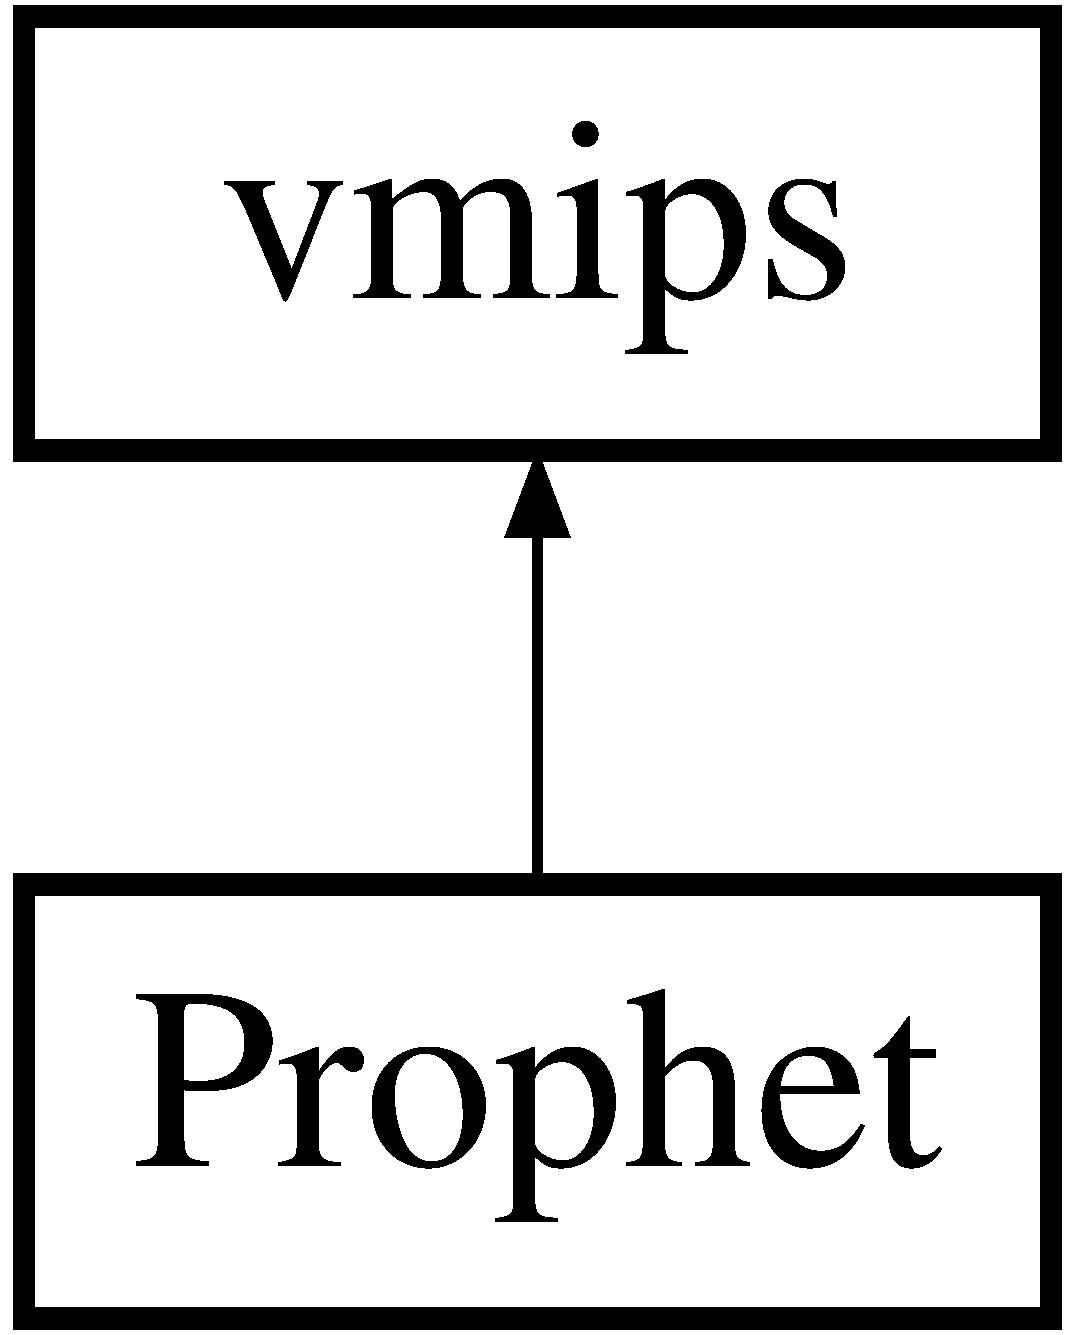
\includegraphics[height=2cm]{classvmips}
\end{center}
\end{figure}
\subsection*{Public Member Functions}
\begin{DoxyCompactItemize}
\item 
\hypertarget{classvmips_a637840190b95211ff10a780e03a9e528}{
void {\bfseries refresh\_\-options} (void)}
\label{classvmips_a637840190b95211ff10a780e03a9e528}

\item 
\hypertarget{classvmips_a7b5449e9f0ba819a3a3364222c8d31d3}{
{\bfseries vmips} (int argc, char $\ast$$\ast$argv)}
\label{classvmips_a7b5449e9f0ba819a3a3364222c8d31d3}

\item 
\hypertarget{classvmips_a69ec3a670b86d802f91157dc791b4617}{
virtual void {\bfseries setup\_\-machine} (void)}
\label{classvmips_a69ec3a670b86d802f91157dc791b4617}

\item 
\hypertarget{classvmips_aa8d4ad6d657ddb10b54b6281a31b0a1c}{
void {\bfseries randomize} (void)}
\label{classvmips_aa8d4ad6d657ddb10b54b6281a31b0a1c}

\item 
\hypertarget{classvmips_a59555b31b9b80731838b73a9fb6d9166}{
void {\bfseries halt} (void)  throw ()}
\label{classvmips_a59555b31b9b80731838b73a9fb6d9166}

\item 
\hypertarget{classvmips_a9d9b546b6cdabd0e813dd7cf8e6a9a12}{
int {\bfseries host\_\-endian\_\-selftest} (void)}
\label{classvmips_a9d9b546b6cdabd0e813dd7cf8e6a9a12}

\item 
\hypertarget{classvmips_a6ba4b580d4069985bcac2dfa653bda2c}{
virtual void {\bfseries step} (void)}
\label{classvmips_a6ba4b580d4069985bcac2dfa653bda2c}

\item 
\hypertarget{classvmips_adf103ab6badbdd18cdd22ba98ac8d9f4}{
virtual int {\bfseries run} (void)}
\label{classvmips_adf103ab6badbdd18cdd22ba98ac8d9f4}

\end{DoxyCompactItemize}
\subsection*{Static Public Member Functions}
\begin{DoxyCompactItemize}
\item 
\hypertarget{classvmips_a4354f7aef601f61d923f8794e73d17aa}{
static uint32 {\bfseries get\_\-file\_\-size} (FILE $\ast$fp)  throw ()}
\label{classvmips_a4354f7aef601f61d923f8794e73d17aa}

\end{DoxyCompactItemize}
\subsection*{Public Attributes}
\begin{DoxyCompactItemize}
\item 
\hypertarget{classvmips_a205bf9dd1afc05f8472862411c5662bc}{
\hyperlink{classMapper}{Mapper} $\ast$ {\bfseries physmem}}
\label{classvmips_a205bf9dd1afc05f8472862411c5662bc}

\item 
\hypertarget{classvmips_a894fc31ccd3e941302d94bfa1ed4ccf2}{
\hyperlink{classCPU}{CPU} $\ast$ {\bfseries cpu}}
\label{classvmips_a894fc31ccd3e941302d94bfa1ed4ccf2}

\item 
\hypertarget{classvmips_a8181ed4a2475f6f46c100e864b43223c}{
\hyperlink{classIntCtrl}{IntCtrl} $\ast$ {\bfseries intc}}
\label{classvmips_a8181ed4a2475f6f46c100e864b43223c}

\item 
\hypertarget{classvmips_a553a8e8bf5c557ab9bf66bd643e7e8b5}{
\hyperlink{classOptions}{Options} $\ast$ {\bfseries opt}}
\label{classvmips_a553a8e8bf5c557ab9bf66bd643e7e8b5}

\item 
\hypertarget{classvmips_ab9df9188bbd2505338201a19552c0cb7}{
\hyperlink{classMemoryModule}{MemoryModule} $\ast$ {\bfseries memmod}}
\label{classvmips_ab9df9188bbd2505338201a19552c0cb7}

\item 
\hypertarget{classvmips_af4540ce57a78b02824f91ab26033e388}{
\hyperlink{classDebug}{Debug} $\ast$ {\bfseries dbgr}}
\label{classvmips_af4540ce57a78b02824f91ab26033e388}

\item 
\hypertarget{classvmips_a6882445296ef06c42b790ca04b9174ab}{
\hyperlink{classDisassembler}{Disassembler} $\ast$ {\bfseries disasm}}
\label{classvmips_a6882445296ef06c42b790ca04b9174ab}

\item 
\hypertarget{classvmips_a8e30b10692502c8dd15d53204fd7b9d5}{
bool {\bfseries host\_\-bigendian}}
\label{classvmips_a8e30b10692502c8dd15d53204fd7b9d5}

\item 
\hypertarget{classvmips_a302365e929db9b1a3a9fc11d2bea5c56}{
bool {\bfseries halted}}
\label{classvmips_a302365e929db9b1a3a9fc11d2bea5c56}

\item 
\hypertarget{classvmips_a514ae1b7c652d4a60afc146d5043b0a0}{
\hyperlink{classDECCSRDevice}{DECCSRDevice} $\ast$ {\bfseries deccsr\_\-device}}
\label{classvmips_a514ae1b7c652d4a60afc146d5043b0a0}

\end{DoxyCompactItemize}
\subsection*{Protected Member Functions}
\begin{DoxyCompactItemize}
\item 
\hypertarget{classvmips_a2e203897ea48f719ff7a3a1007fcf0fe}{
virtual void {\bfseries boot\_\-msg} (const char $\ast$msg,...)  throw ()}
\label{classvmips_a2e203897ea48f719ff7a3a1007fcf0fe}

\item 
\hypertarget{classvmips_ab3966b7e461c76e01e1794c2302c1264}{
virtual bool {\bfseries setup\_\-spimconsole} ()  throw (std::bad\_\-alloc)}
\label{classvmips_ab3966b7e461c76e01e1794c2302c1264}

\item 
\hypertarget{classvmips_a1690e2f7dc015006579396258fc9ec09}{
virtual bool {\bfseries setup\_\-clockdevice} ()  throw ( std::bad\_\-alloc )}
\label{classvmips_a1690e2f7dc015006579396258fc9ec09}

\item 
\hypertarget{classvmips_aaca514986ff2099e5b2749b38b5b83de}{
virtual bool {\bfseries setup\_\-decrtc} ()  throw ( std::bad\_\-alloc )}
\label{classvmips_aaca514986ff2099e5b2749b38b5b83de}

\item 
\hypertarget{classvmips_a11077bfbc7b6851733526afcd6bc0511}{
virtual bool {\bfseries setup\_\-deccsr} ()  throw ( std::bad\_\-alloc )}
\label{classvmips_a11077bfbc7b6851733526afcd6bc0511}

\item 
\hypertarget{classvmips_a064bd152d3a1a003f9190cfec219fd48}{
virtual bool {\bfseries setup\_\-decstat} ()  throw ( std::bad\_\-alloc )}
\label{classvmips_a064bd152d3a1a003f9190cfec219fd48}

\item 
\hypertarget{classvmips_a6f7b8aacf8a8ab3ff1b58f0c4e7e2450}{
virtual bool {\bfseries setup\_\-decserial} ()  throw ( std::bad\_\-alloc )}
\label{classvmips_a6f7b8aacf8a8ab3ff1b58f0c4e7e2450}

\item 
\hypertarget{classvmips_adaf982c53a952510e342b6c20f6a07fa}{
virtual bool {\bfseries setup\_\-rom} ()}
\label{classvmips_adaf982c53a952510e342b6c20f6a07fa}

\item 
\hypertarget{classvmips_affc49823a8f7c7b01313208eeab24958}{
virtual bool {\bfseries setup\_\-exe} ()}
\label{classvmips_affc49823a8f7c7b01313208eeab24958}

\item 
\hypertarget{classvmips_a1174dbe6a6e0318145c2aeaee01c4a93}{
bool {\bfseries load\_\-elf} (FILE $\ast$fp)}
\label{classvmips_a1174dbe6a6e0318145c2aeaee01c4a93}

\item 
\hypertarget{classvmips_a4476a0bc2039e7a43ec2208d7ae5addb}{
bool {\bfseries load\_\-ecoff} (FILE $\ast$fp)}
\label{classvmips_a4476a0bc2039e7a43ec2208d7ae5addb}

\item 
char $\ast$ \hyperlink{classvmips_aca7c30f28c9be1cbf9d0780d66d3393c}{translate\_\-to\_\-host\_\-ram\_\-pointer} (uint32 vaddr)
\item 
\hypertarget{classvmips_a8374e36944913b2a41f9a72bef18f691}{
virtual bool {\bfseries setup\_\-ram} ()  throw (std::bad\_\-alloc)}
\label{classvmips_a8374e36944913b2a41f9a72bef18f691}

\item 
\hypertarget{classvmips_a2ede92940f80c240d6550987d280a39b}{
virtual bool {\bfseries setup\_\-clock} ()  throw (std::bad\_\-alloc)}
\label{classvmips_a2ede92940f80c240d6550987d280a39b}

\item 
\hypertarget{classvmips_a441e17463fe05a71a960e1f98f11019b}{
virtual void {\bfseries setup\_\-console\_\-line} (int l, char $\ast$name, \hyperlink{classTerminalController}{TerminalController} $\ast$c, const char $\ast$c\_\-name)  throw ()}
\label{classvmips_a441e17463fe05a71a960e1f98f11019b}

\item 
\hypertarget{classvmips_ace907fda17fe54e632f871ba19405744}{
bool {\bfseries setup\_\-haltdevice} ()  throw ( std::bad\_\-alloc )}
\label{classvmips_ace907fda17fe54e632f871ba19405744}

\end{DoxyCompactItemize}
\subsection*{Protected Attributes}
\begin{DoxyCompactItemize}
\item 
\hypertarget{classvmips_a0953c7ad4349b5cf5c4396b0b85d6aba}{
\hyperlink{classClock}{Clock} $\ast$ {\bfseries clock}}
\label{classvmips_a0953c7ad4349b5cf5c4396b0b85d6aba}

\item 
\hypertarget{classvmips_a5434d8b73ef3d316e3c7c254ef445028}{
\hyperlink{classClockDevice}{ClockDevice} $\ast$ {\bfseries clock\_\-device}}
\label{classvmips_a5434d8b73ef3d316e3c7c254ef445028}

\item 
\hypertarget{classvmips_a1e36783bf8b1e79e8b6d5b34feaf12db}{
\hyperlink{classHaltDevice}{HaltDevice} $\ast$ {\bfseries halt\_\-device}}
\label{classvmips_a1e36783bf8b1e79e8b6d5b34feaf12db}

\item 
\hypertarget{classvmips_aa51d2bbd33d18409ff22698c4cd6f924}{
\hyperlink{classSpimConsoleDevice}{SpimConsoleDevice} $\ast$ {\bfseries spim\_\-console}}
\label{classvmips_aa51d2bbd33d18409ff22698c4cd6f924}

\item 
\hypertarget{classvmips_ae94fc21627cb58c51d2924ac34fc159a}{
\hyperlink{classDECRTCDevice}{DECRTCDevice} $\ast$ {\bfseries decrtc\_\-device}}
\label{classvmips_ae94fc21627cb58c51d2924ac34fc159a}

\item 
\hypertarget{classvmips_a65a336362e2697c44e29ac552956e601}{
\hyperlink{classDECStatDevice}{DECStatDevice} $\ast$ {\bfseries decstat\_\-device}}
\label{classvmips_a65a336362e2697c44e29ac552956e601}

\item 
\hypertarget{classvmips_ac048b9d198c5c6aa60bd08b1cae9c589}{
\hyperlink{classDECSerialDevice}{DECSerialDevice} $\ast$ {\bfseries decserial\_\-device}}
\label{classvmips_ac048b9d198c5c6aa60bd08b1cae9c589}

\item 
\hypertarget{classvmips_a562fa4cb239eac6ea40f91acd5be8842}{
bool {\bfseries opt\_\-bootmsg}}
\label{classvmips_a562fa4cb239eac6ea40f91acd5be8842}

\item 
\hypertarget{classvmips_a0b4556b2e97d14a33240e6712700fea2}{
bool {\bfseries opt\_\-clockdevice}}
\label{classvmips_a0b4556b2e97d14a33240e6712700fea2}

\item 
\hypertarget{classvmips_ae17758697d6d44d04f19a9f269ccadbe}{
bool {\bfseries opt\_\-debug}}
\label{classvmips_ae17758697d6d44d04f19a9f269ccadbe}

\item 
\hypertarget{classvmips_a46e7e40fb65be2d316f8b317e63f849c}{
bool {\bfseries opt\_\-dumpcpu}}
\label{classvmips_a46e7e40fb65be2d316f8b317e63f849c}

\item 
\hypertarget{classvmips_add942d2c47c4dbb52336775165019697}{
bool {\bfseries opt\_\-dumpcp0}}
\label{classvmips_add942d2c47c4dbb52336775165019697}

\item 
\hypertarget{classvmips_a50549bb2d6a97523ad12ba30cf5b71f7}{
bool {\bfseries opt\_\-haltdevice}}
\label{classvmips_a50549bb2d6a97523ad12ba30cf5b71f7}

\item 
\hypertarget{classvmips_a4a6b2c9d6271460231b461d93027a3e8}{
bool {\bfseries opt\_\-haltdumpcpu}}
\label{classvmips_a4a6b2c9d6271460231b461d93027a3e8}

\item 
\hypertarget{classvmips_aeadd614ab54a14c44976cfb6ff1e945a}{
bool {\bfseries opt\_\-haltdumpcp0}}
\label{classvmips_aeadd614ab54a14c44976cfb6ff1e945a}

\item 
\hypertarget{classvmips_adf13dd6895b81ce6070edf9aebde1cc2}{
bool {\bfseries opt\_\-instcounts}}
\label{classvmips_adf13dd6895b81ce6070edf9aebde1cc2}

\item 
\hypertarget{classvmips_a241d92d606f1578fbd7d8a965adffbf4}{
bool {\bfseries opt\_\-memdump}}
\label{classvmips_a241d92d606f1578fbd7d8a965adffbf4}

\item 
\hypertarget{classvmips_a67853be6d92b63df5be4ab5f995af92c}{
bool {\bfseries opt\_\-realtime}}
\label{classvmips_a67853be6d92b63df5be4ab5f995af92c}

\item 
\hypertarget{classvmips_a6d1bbb851cbd3f42e345c53168885d67}{
bool {\bfseries opt\_\-decrtc}}
\label{classvmips_a6d1bbb851cbd3f42e345c53168885d67}

\item 
\hypertarget{classvmips_ad4fad72fddd561a9b911ff1517f2d0e2}{
bool {\bfseries opt\_\-deccsr}}
\label{classvmips_ad4fad72fddd561a9b911ff1517f2d0e2}

\item 
\hypertarget{classvmips_afd847beb4fd38de8749d64b08484c74c}{
bool {\bfseries opt\_\-decstat}}
\label{classvmips_afd847beb4fd38de8749d64b08484c74c}

\item 
\hypertarget{classvmips_a1c0b2005865aa0fef47900fd15f0f101}{
bool {\bfseries opt\_\-decserial}}
\label{classvmips_a1c0b2005865aa0fef47900fd15f0f101}

\item 
\hypertarget{classvmips_ac83c39cf33c020edc6a4ecb62b83fd66}{
bool {\bfseries opt\_\-spimconsole}}
\label{classvmips_ac83c39cf33c020edc6a4ecb62b83fd66}

\item 
\hypertarget{classvmips_a509accc98158cb32497aaa73c064f5ad}{
uint32 {\bfseries opt\_\-clockspeed}}
\label{classvmips_a509accc98158cb32497aaa73c064f5ad}

\item 
\hypertarget{classvmips_a0233d4fb0ecc150e915c8df3b86d6c7a}{
uint32 {\bfseries clock\_\-nanos}}
\label{classvmips_a0233d4fb0ecc150e915c8df3b86d6c7a}

\item 
\hypertarget{classvmips_ac0d668e4be7fbe09a58bc2212c9364b7}{
uint32 {\bfseries opt\_\-clockintr}}
\label{classvmips_ac0d668e4be7fbe09a58bc2212c9364b7}

\item 
\hypertarget{classvmips_af1707a050c33609fc873632e1a9a7f38}{
uint32 {\bfseries opt\_\-clockdeviceirq}}
\label{classvmips_af1707a050c33609fc873632e1a9a7f38}

\item 
\hypertarget{classvmips_ad10ae1ddb3f0f3e6f8c8d6702c04cca9}{
uint32 {\bfseries opt\_\-loadaddr}}
\label{classvmips_ad10ae1ddb3f0f3e6f8c8d6702c04cca9}

\item 
\hypertarget{classvmips_a6c58f9361ce92d3286ad2f26ede4c5b8}{
uint32 {\bfseries opt\_\-memsize}}
\label{classvmips_a6c58f9361ce92d3286ad2f26ede4c5b8}

\item 
\hypertarget{classvmips_aced781c93879f5a69c4721753a35949a}{
uint32 {\bfseries opt\_\-timeratio}}
\label{classvmips_aced781c93879f5a69c4721753a35949a}

\item 
\hypertarget{classvmips_a52bbd49d9f9198be2774298f9822c6b9}{
char $\ast$ {\bfseries opt\_\-image}}
\label{classvmips_a52bbd49d9f9198be2774298f9822c6b9}

\item 
\hypertarget{classvmips_a85a78486d34873c71b5a38ec0d7c95cd}{
char $\ast$ {\bfseries opt\_\-execname}}
\label{classvmips_a85a78486d34873c71b5a38ec0d7c95cd}

\item 
\hypertarget{classvmips_a8cd1c860c1cb22767a3778330f18cdcc}{
char $\ast$ {\bfseries opt\_\-memdumpfile}}
\label{classvmips_a8cd1c860c1cb22767a3778330f18cdcc}

\item 
\hypertarget{classvmips_a174b8c59d240d8d8c69b07ae34d2b896}{
char $\ast$ {\bfseries opt\_\-ttydev}}
\label{classvmips_a174b8c59d240d8d8c69b07ae34d2b896}

\item 
\hypertarget{classvmips_ab9e2192b3fe2b29179fa01142055e2a6}{
char $\ast$ {\bfseries opt\_\-ttydev2}}
\label{classvmips_ab9e2192b3fe2b29179fa01142055e2a6}

\end{DoxyCompactItemize}


\subsection{Member Function Documentation}
\hypertarget{classvmips_aca7c30f28c9be1cbf9d0780d66d3393c}{
\index{vmips@{vmips}!translate\_\-to\_\-host\_\-ram\_\-pointer@{translate\_\-to\_\-host\_\-ram\_\-pointer}}
\index{translate\_\-to\_\-host\_\-ram\_\-pointer@{translate\_\-to\_\-host\_\-ram\_\-pointer}!vmips@{vmips}}
\subsubsection[{translate\_\-to\_\-host\_\-ram\_\-pointer}]{\setlength{\rightskip}{0pt plus 5cm}char $\ast$ vmips::translate\_\-to\_\-host\_\-ram\_\-pointer (uint32 {\em vaddr})\hspace{0.3cm}{\ttfamily  \mbox{[}protected\mbox{]}}}}
\label{classvmips_aca7c30f28c9be1cbf9d0780d66d3393c}
Translate vaddr to a physical address, then return a host-\/machine pointer to where it is in the simulated machine's RAM. vaddr must be in one of the non-\/mapped kernel-\/mode segments (KSEG0 or KSEG1), and it must be within the bounds of the simulated machine's physical RAM. Otherwise a null pointer is returned. 

The documentation for this class was generated from the following files:\begin{DoxyCompactItemize}
\item 
vmips.h\item 
exeloader.cc\item 
vmips.cc\end{DoxyCompactItemize}

\hypertarget{classVmipstoolOptions}{
\section{VmipstoolOptions Class Reference}
\label{classVmipstoolOptions}\index{VmipstoolOptions@{VmipstoolOptions}}
}
Inheritance diagram for VmipstoolOptions:\begin{figure}[H]
\begin{center}
\leavevmode
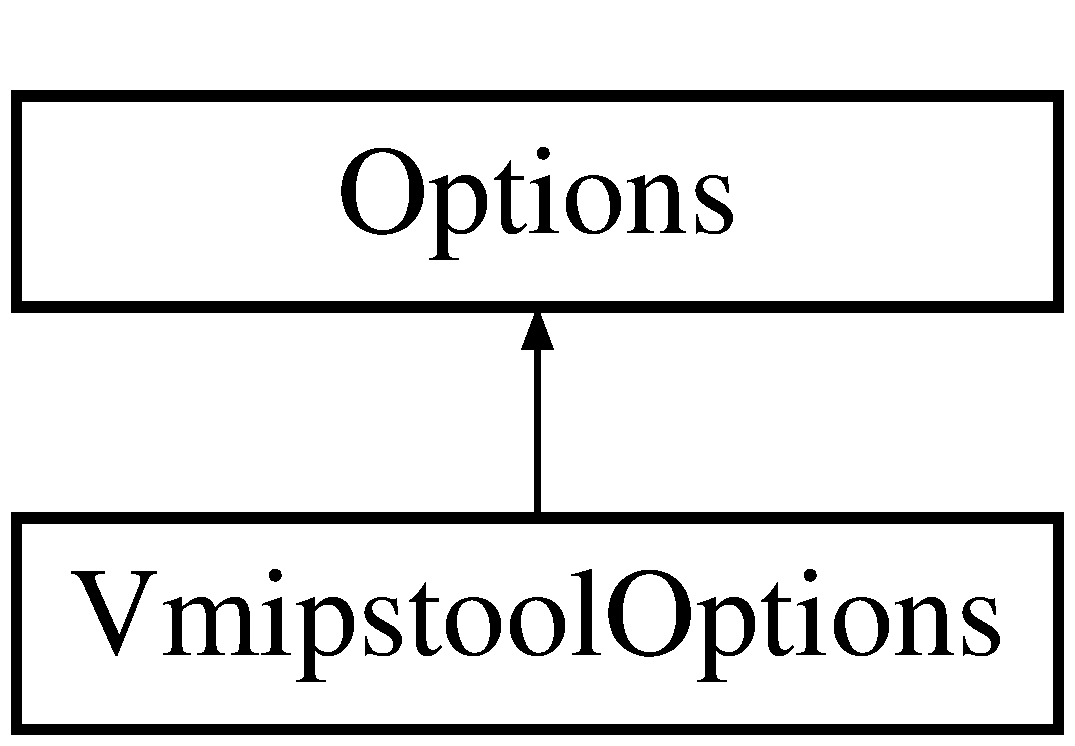
\includegraphics[height=2cm]{classVmipstoolOptions}
\end{center}
\end{figure}
\subsection*{Public Member Functions}
\begin{DoxyCompactItemize}
\item 
\hypertarget{classVmipstoolOptions_a0b491d0ea280503ddfa10301ead352a9}{
virtual void {\bfseries usage} (char $\ast$argv0)}
\label{classVmipstoolOptions_a0b491d0ea280503ddfa10301ead352a9}

\item 
\hypertarget{classVmipstoolOptions_a97de4ae758e6967ec609d53c828a6b05}{
virtual void {\bfseries process\_\-options} (int argc, char $\ast$$\ast$argv)}
\label{classVmipstoolOptions_a97de4ae758e6967ec609d53c828a6b05}

\end{DoxyCompactItemize}


The documentation for this class was generated from the following file:\begin{DoxyCompactItemize}
\item 
vmipstool.cc\end{DoxyCompactItemize}

\hypertarget{classXmlDocument}{
\section{XmlDocument Class Reference}
\label{classXmlDocument}\index{XmlDocument@{XmlDocument}}
}


A XML Document.  




{\ttfamily \#include $<$prophetxmldoc.h$>$}

\subsection*{Public Member Functions}
\begin{DoxyCompactItemize}
\item 
\hyperlink{classXmlDocument_a3bc4c5ea5f22b4ff8776422125b31d42}{XmlDocument} (const std::string \&encoding=\char`\"{}\char`\"{}, const std::string \&styleSheet=\char`\"{}\char`\"{})
\begin{DoxyCompactList}\small\item\em Constructs a \hyperlink{classXmlDocument}{XmlDocument} object. \item\end{DoxyCompactList}\item 
\hypertarget{classXmlDocument_ab18742228f580a5e4ec87e4b39c8a68c}{
virtual \hyperlink{classXmlDocument_ab18742228f580a5e4ec87e4b39c8a68c}{$\sim$XmlDocument} ()}
\label{classXmlDocument_ab18742228f580a5e4ec87e4b39c8a68c}

\begin{DoxyCompactList}\small\item\em Destructor. \item\end{DoxyCompactList}\item 
\hypertarget{classXmlDocument_a5063b9dc310ed5ed7a38b77f8584a50c}{
std::string {\bfseries encoding} () const }
\label{classXmlDocument_a5063b9dc310ed5ed7a38b77f8584a50c}

\item 
\hypertarget{classXmlDocument_afb4401e77f67626533ba7409a011c508}{
void {\bfseries setEncoding} (const std::string \&encoding=\char`\"{}\char`\"{})}
\label{classXmlDocument_afb4401e77f67626533ba7409a011c508}

\item 
\hypertarget{classXmlDocument_ae0a7e5e1f28b179c31bee66481b18c03}{
std::string {\bfseries styleSheet} () const }
\label{classXmlDocument_ae0a7e5e1f28b179c31bee66481b18c03}

\item 
\hypertarget{classXmlDocument_a63cfdd276a9812900cd7739758effd78}{
void {\bfseries setStyleSheet} (const std::string \&styleSheet=\char`\"{}\char`\"{})}
\label{classXmlDocument_a63cfdd276a9812900cd7739758effd78}

\item 
\hypertarget{classXmlDocument_ab3ff5eb5c5df20453b4fc6f5b9bcff6e}{
bool {\bfseries standalone} () const }
\label{classXmlDocument_ab3ff5eb5c5df20453b4fc6f5b9bcff6e}

\item 
void \hyperlink{classXmlDocument_a3cc9d3452daba0bda758ee7add075827}{setStandalone} (bool standalone)
\begin{DoxyCompactList}\small\item\em set the output document as standalone or not. \item\end{DoxyCompactList}\item 
\hypertarget{classXmlDocument_a2b419770905e48914ed6dba3990061cd}{
void {\bfseries setRootElement} (\hyperlink{classXmlElement}{XmlElement} $\ast$rootElement)}
\label{classXmlDocument_a2b419770905e48914ed6dba3990061cd}

\item 
\hypertarget{classXmlDocument_a23a48b334d0ab31d4d68a489d0c60acc}{
\hyperlink{classXmlElement}{XmlElement} \& {\bfseries rootElement} () const }
\label{classXmlDocument_a23a48b334d0ab31d4d68a489d0c60acc}

\item 
\hypertarget{classXmlDocument_aa75e20c19ee0719af2e5b573db02f5a4}{
std::string {\bfseries toString} () const }
\label{classXmlDocument_aa75e20c19ee0719af2e5b573db02f5a4}

\end{DoxyCompactItemize}
\subsection*{Protected Attributes}
\begin{DoxyCompactItemize}
\item 
\hypertarget{classXmlDocument_a3a5338a6b02b176a3d50e6665ce1b41d}{
std::string {\bfseries m\_\-encoding}}
\label{classXmlDocument_a3a5338a6b02b176a3d50e6665ce1b41d}

\item 
\hypertarget{classXmlDocument_a8564bf7c7d4856e6aecc2d7b7be6782b}{
std::string {\bfseries m\_\-styleSheet}}
\label{classXmlDocument_a8564bf7c7d4856e6aecc2d7b7be6782b}

\item 
\hypertarget{classXmlDocument_a83e49d668c247017d1681a9989958280}{
\hyperlink{classXmlElement}{XmlElement} $\ast$ {\bfseries m\_\-rootElement}}
\label{classXmlDocument_a83e49d668c247017d1681a9989958280}

\item 
\hypertarget{classXmlDocument_a0c2dd2a48772ad62209a268156af3baa}{
bool {\bfseries m\_\-standalone}}
\label{classXmlDocument_a0c2dd2a48772ad62209a268156af3baa}

\end{DoxyCompactItemize}


\subsection{Detailed Description}
A XML Document. A \hyperlink{classXmlDocument}{XmlDocument} represents a XML file. It holds a pointer on the root \hyperlink{classXmlElement}{XmlElement} of the document. It also holds the encoding and style sheet used.

By default, the XML document is stand-\/alone and tagged with enconding \char`\"{}ISO-\/8859-\/1\char`\"{}. 

\subsection{Constructor \& Destructor Documentation}
\hypertarget{classXmlDocument_a3bc4c5ea5f22b4ff8776422125b31d42}{
\index{XmlDocument@{XmlDocument}!XmlDocument@{XmlDocument}}
\index{XmlDocument@{XmlDocument}!XmlDocument@{XmlDocument}}
\subsubsection[{XmlDocument}]{\setlength{\rightskip}{0pt plus 5cm}XmlDocument::XmlDocument (const std::string \& {\em encoding} = {\ttfamily \char`\"{}\char`\"{}}, \/  const std::string \& {\em styleSheet} = {\ttfamily \char`\"{}\char`\"{}})}}
\label{classXmlDocument_a3bc4c5ea5f22b4ff8776422125b31d42}


Constructs a \hyperlink{classXmlDocument}{XmlDocument} object. 


\begin{DoxyParams}{Parameters}
\item[{\em encoding}]Encoding used in the XML file (default is Latin-\/1, ISO-\/8859-\/1 ). \item[{\em styleSheet}]Name of the XSL style sheet file used. If empty then no style sheet will be specified in the output. \end{DoxyParams}


\subsection{Member Function Documentation}
\hypertarget{classXmlDocument_a3cc9d3452daba0bda758ee7add075827}{
\index{XmlDocument@{XmlDocument}!setStandalone@{setStandalone}}
\index{setStandalone@{setStandalone}!XmlDocument@{XmlDocument}}
\subsubsection[{setStandalone}]{\setlength{\rightskip}{0pt plus 5cm}void XmlDocument::setStandalone (bool {\em standalone})}}
\label{classXmlDocument_a3cc9d3452daba0bda758ee7add075827}


set the output document as standalone or not. 

For the output document, specify wether it's a standalone XML document, or not.


\begin{DoxyParams}{Parameters}
\item[{\em standalone}]if true, the output will be specified as standalone. if false, it will be not. \end{DoxyParams}


The documentation for this class was generated from the following files:\begin{DoxyCompactItemize}
\item 
prophetxmldoc.h\item 
prophetxmldoc.cc\end{DoxyCompactItemize}

\hypertarget{classXmlElement}{
\section{XmlElement Class Reference}
\label{classXmlElement}\index{XmlElement@{XmlElement}}
}


A XML Element.  




{\ttfamily \#include $<$prophetxmlelement.h$>$}

\subsection*{Public Member Functions}
\begin{DoxyCompactItemize}
\item 
\hyperlink{classXmlElement_a94d6c15e996994d62316b198f369d675}{XmlElement} (std::string elementName, std::string content=\char`\"{}\char`\"{})
\begin{DoxyCompactList}\small\item\em Constructs an element with the specified name and string content. \item\end{DoxyCompactList}\item 
\hyperlink{classXmlElement_a879b90d96dc87b6f7ebb9c67ba92cb73}{XmlElement} (std::string elementName, int numericContent)
\begin{DoxyCompactList}\small\item\em Constructs an element with the specified name and numeric content. \item\end{DoxyCompactList}\item 
\hypertarget{classXmlElement_a1e67b1dfcd561d1d602988d100d80d9b}{
virtual \hyperlink{classXmlElement_a1e67b1dfcd561d1d602988d100d80d9b}{$\sim$XmlElement} ()}
\label{classXmlElement_a1e67b1dfcd561d1d602988d100d80d9b}

\begin{DoxyCompactList}\small\item\em Destructs the element and its child elements. \item\end{DoxyCompactList}\item 
std::string \hyperlink{classXmlElement_a924c45bc90419123174ac9d11089cb6d}{name} () const 
\begin{DoxyCompactList}\small\item\em Returns the name of the element. \item\end{DoxyCompactList}\item 
std::string \hyperlink{classXmlElement_a3fea4e46ca4e63ceb905a96a8f304381}{content} () const 
\begin{DoxyCompactList}\small\item\em Returns the content of the element. \item\end{DoxyCompactList}\item 
void \hyperlink{classXmlElement_a0ed6ad08fd972865cca13ae2594fedda}{setName} (const std::string \&name)
\begin{DoxyCompactList}\small\item\em Sets the name of the element. \item\end{DoxyCompactList}\item 
void \hyperlink{classXmlElement_aaf32abf7cdaf31b8896f52a7859d9826}{setContent} (const std::string \&content)
\begin{DoxyCompactList}\small\item\em Sets the content of the element. \item\end{DoxyCompactList}\item 
\hypertarget{classXmlElement_ae8d473f1d193157158ae36e12929d387}{
void {\bfseries setContent} (int numericContent)}
\label{classXmlElement_ae8d473f1d193157158ae36e12929d387}

\item 
void \hyperlink{classXmlElement_a14387be9ca6d014a38e95a7aa98f86c5}{addAttribute} (std::string attributeName, std::string value)
\begin{DoxyCompactList}\small\item\em Adds an attribute with the specified string value. \item\end{DoxyCompactList}\item 
void \hyperlink{classXmlElement_aec69fb49cf9e563cff9858ddc818f055}{addAttribute} (std::string attributeName, int numericValue)
\begin{DoxyCompactList}\small\item\em Adds an attribute with the specified numeric value. \item\end{DoxyCompactList}\item 
void \hyperlink{classXmlElement_a444321a1de2a7f52994c53f9e6e0d942}{addElement} (\hyperlink{classXmlElement}{XmlElement} $\ast$element)
\begin{DoxyCompactList}\small\item\em Adds a child element to the element. \item\end{DoxyCompactList}\item 
int \hyperlink{classXmlElement_a2aad0dda599cb46f85ff6b4b897045b9}{elementCount} () const 
\begin{DoxyCompactList}\small\item\em Returns the number of child elements. \item\end{DoxyCompactList}\item 
\hyperlink{classXmlElement}{XmlElement} $\ast$ \hyperlink{classXmlElement_a083d56e5d6e8ef4f4ed462b3206b3af2}{elementAt} (int index) const 
\begin{DoxyCompactList}\small\item\em Returns the child element at the specified index. \item\end{DoxyCompactList}\item 
\hyperlink{classXmlElement}{XmlElement} $\ast$ \hyperlink{classXmlElement_a6babcb48cd31c025234ad35db5ebce3e}{elementFor} (const std::string \&name) const 
\begin{DoxyCompactList}\small\item\em Returns the first child element with the specified name. \item\end{DoxyCompactList}\item 
std::string \hyperlink{classXmlElement_a2e783a5fed6b5b31b2d11117e6c83d40}{toString} (const std::string \&indent=\char`\"{}\char`\"{}) const 
\begin{DoxyCompactList}\small\item\em Returns a XML string that represents the element. \item\end{DoxyCompactList}\end{DoxyCompactItemize}


\subsection{Detailed Description}
A XML Element. A XML element has:
\begin{DoxyItemize}
\item a name, specified on construction,
\item a content, specified on construction (may be empty),
\item zero or more attributes, added with \hyperlink{classXmlElement_a14387be9ca6d014a38e95a7aa98f86c5}{addAttribute()},
\item zero or more child elements, added with \hyperlink{classXmlElement_a444321a1de2a7f52994c53f9e6e0d942}{addElement()}. 
\end{DoxyItemize}

\subsection{Constructor \& Destructor Documentation}
\hypertarget{classXmlElement_a94d6c15e996994d62316b198f369d675}{
\index{XmlElement@{XmlElement}!XmlElement@{XmlElement}}
\index{XmlElement@{XmlElement}!XmlElement@{XmlElement}}
\subsubsection[{XmlElement}]{\setlength{\rightskip}{0pt plus 5cm}XmlElement::XmlElement (std::string {\em elementName}, \/  std::string {\em content} = {\ttfamily \char`\"{}\char`\"{}})}}
\label{classXmlElement_a94d6c15e996994d62316b198f369d675}


Constructs an element with the specified name and string content. 


\begin{DoxyParams}{Parameters}
\item[{\em elementName}]Name of the element. Must not be empty. \item[{\em content}]Content of the element. \end{DoxyParams}
\hypertarget{classXmlElement_a879b90d96dc87b6f7ebb9c67ba92cb73}{
\index{XmlElement@{XmlElement}!XmlElement@{XmlElement}}
\index{XmlElement@{XmlElement}!XmlElement@{XmlElement}}
\subsubsection[{XmlElement}]{\setlength{\rightskip}{0pt plus 5cm}XmlElement::XmlElement (std::string {\em elementName}, \/  int {\em numericContent})}}
\label{classXmlElement_a879b90d96dc87b6f7ebb9c67ba92cb73}


Constructs an element with the specified name and numeric content. 


\begin{DoxyParams}{Parameters}
\item[{\em elementName}]Name of the element. Must not be empty. \item[{\em numericContent}]Content of the element. \end{DoxyParams}


\subsection{Member Function Documentation}
\hypertarget{classXmlElement_aec69fb49cf9e563cff9858ddc818f055}{
\index{XmlElement@{XmlElement}!addAttribute@{addAttribute}}
\index{addAttribute@{addAttribute}!XmlElement@{XmlElement}}
\subsubsection[{addAttribute}]{\setlength{\rightskip}{0pt plus 5cm}void XmlElement::addAttribute (std::string {\em attributeName}, \/  int {\em numericValue})}}
\label{classXmlElement_aec69fb49cf9e563cff9858ddc818f055}


Adds an attribute with the specified numeric value. 


\begin{DoxyParams}{Parameters}
\item[{\em attributeName}]Name of the attribute. Must not be empty. \item[{\em numericValue}]Numeric value of the attribute. \end{DoxyParams}
\hypertarget{classXmlElement_a14387be9ca6d014a38e95a7aa98f86c5}{
\index{XmlElement@{XmlElement}!addAttribute@{addAttribute}}
\index{addAttribute@{addAttribute}!XmlElement@{XmlElement}}
\subsubsection[{addAttribute}]{\setlength{\rightskip}{0pt plus 5cm}void XmlElement::addAttribute (std::string {\em attributeName}, \/  std::string {\em value})}}
\label{classXmlElement_a14387be9ca6d014a38e95a7aa98f86c5}


Adds an attribute with the specified string value. 


\begin{DoxyParams}{Parameters}
\item[{\em attributeName}]Name of the attribute. Must not be an empty. \item[{\em value}]Value of the attribute. \end{DoxyParams}
\hypertarget{classXmlElement_a444321a1de2a7f52994c53f9e6e0d942}{
\index{XmlElement@{XmlElement}!addElement@{addElement}}
\index{addElement@{addElement}!XmlElement@{XmlElement}}
\subsubsection[{addElement}]{\setlength{\rightskip}{0pt plus 5cm}void XmlElement::addElement ({\bf XmlElement} $\ast$ {\em element})}}
\label{classXmlElement_a444321a1de2a7f52994c53f9e6e0d942}


Adds a child element to the element. 


\begin{DoxyParams}{Parameters}
\item[{\em element}]Child element to add. Must not be {\ttfamily NULL}. \end{DoxyParams}
\hypertarget{classXmlElement_a3fea4e46ca4e63ceb905a96a8f304381}{
\index{XmlElement@{XmlElement}!content@{content}}
\index{content@{content}!XmlElement@{XmlElement}}
\subsubsection[{content}]{\setlength{\rightskip}{0pt plus 5cm}std::string XmlElement::content () const}}
\label{classXmlElement_a3fea4e46ca4e63ceb905a96a8f304381}


Returns the content of the element. 

\begin{DoxyReturn}{Returns}
Content of the element. 
\end{DoxyReturn}
\hypertarget{classXmlElement_a083d56e5d6e8ef4f4ed462b3206b3af2}{
\index{XmlElement@{XmlElement}!elementAt@{elementAt}}
\index{elementAt@{elementAt}!XmlElement@{XmlElement}}
\subsubsection[{elementAt}]{\setlength{\rightskip}{0pt plus 5cm}{\bf XmlElement} $\ast$ XmlElement::elementAt (int {\em index}) const}}
\label{classXmlElement_a083d56e5d6e8ef4f4ed462b3206b3af2}


Returns the child element at the specified index. 


\begin{DoxyParams}{Parameters}
\item[{\em index}]Zero based index of the element to return. \end{DoxyParams}
\begin{DoxyReturn}{Returns}
Element at the specified index. Never {\ttfamily NULL}. 
\end{DoxyReturn}

\begin{DoxyExceptions}{Exceptions}
\item[{\em std::invalid\_\-argument}]if {\itshape index\/} $<$ 0 or index $>$= \hyperlink{classXmlElement_a2aad0dda599cb46f85ff6b4b897045b9}{elementCount()}. \end{DoxyExceptions}
\hypertarget{classXmlElement_a2aad0dda599cb46f85ff6b4b897045b9}{
\index{XmlElement@{XmlElement}!elementCount@{elementCount}}
\index{elementCount@{elementCount}!XmlElement@{XmlElement}}
\subsubsection[{elementCount}]{\setlength{\rightskip}{0pt plus 5cm}int XmlElement::elementCount () const}}
\label{classXmlElement_a2aad0dda599cb46f85ff6b4b897045b9}


Returns the number of child elements. 

\begin{DoxyReturn}{Returns}
Number of child elements (element added with \hyperlink{classXmlElement_a444321a1de2a7f52994c53f9e6e0d942}{addElement()}). 
\end{DoxyReturn}
\hypertarget{classXmlElement_a6babcb48cd31c025234ad35db5ebce3e}{
\index{XmlElement@{XmlElement}!elementFor@{elementFor}}
\index{elementFor@{elementFor}!XmlElement@{XmlElement}}
\subsubsection[{elementFor}]{\setlength{\rightskip}{0pt plus 5cm}{\bf XmlElement} $\ast$ XmlElement::elementFor (const std::string \& {\em name}) const}}
\label{classXmlElement_a6babcb48cd31c025234ad35db5ebce3e}


Returns the first child element with the specified name. 


\begin{DoxyParams}{Parameters}
\item[{\em name}]Name of the child element to return. \end{DoxyParams}
\begin{DoxyReturn}{Returns}
First child element found which is named {\itshape name\/}. 
\end{DoxyReturn}

\begin{DoxyExceptions}{Exceptions}
\item[{\em std::invalid\_\-argument}]if there is no child element with the specified name. \end{DoxyExceptions}
\hypertarget{classXmlElement_a924c45bc90419123174ac9d11089cb6d}{
\index{XmlElement@{XmlElement}!name@{name}}
\index{name@{name}!XmlElement@{XmlElement}}
\subsubsection[{name}]{\setlength{\rightskip}{0pt plus 5cm}std::string XmlElement::name () const}}
\label{classXmlElement_a924c45bc90419123174ac9d11089cb6d}


Returns the name of the element. 

\begin{DoxyReturn}{Returns}
Name of the element. 
\end{DoxyReturn}
\hypertarget{classXmlElement_aaf32abf7cdaf31b8896f52a7859d9826}{
\index{XmlElement@{XmlElement}!setContent@{setContent}}
\index{setContent@{setContent}!XmlElement@{XmlElement}}
\subsubsection[{setContent}]{\setlength{\rightskip}{0pt plus 5cm}void XmlElement::setContent (const std::string \& {\em content})}}
\label{classXmlElement_aaf32abf7cdaf31b8896f52a7859d9826}


Sets the content of the element. 


\begin{DoxyParams}{Parameters}
\item[{\em content}]New content for the element.\end{DoxyParams}
This is an overloaded member function, provided for convenience. It differs from the above function only in what argument(s) it accepts. \hypertarget{classXmlElement_a0ed6ad08fd972865cca13ae2594fedda}{
\index{XmlElement@{XmlElement}!setName@{setName}}
\index{setName@{setName}!XmlElement@{XmlElement}}
\subsubsection[{setName}]{\setlength{\rightskip}{0pt plus 5cm}void XmlElement::setName (const std::string \& {\em name})}}
\label{classXmlElement_a0ed6ad08fd972865cca13ae2594fedda}


Sets the name of the element. 


\begin{DoxyParams}{Parameters}
\item[{\em name}]New name for the element. \end{DoxyParams}
\hypertarget{classXmlElement_a2e783a5fed6b5b31b2d11117e6c83d40}{
\index{XmlElement@{XmlElement}!toString@{toString}}
\index{toString@{toString}!XmlElement@{XmlElement}}
\subsubsection[{toString}]{\setlength{\rightskip}{0pt plus 5cm}std::string XmlElement::toString (const std::string \& {\em indent} = {\ttfamily \char`\"{}\char`\"{}}) const}}
\label{classXmlElement_a2e783a5fed6b5b31b2d11117e6c83d40}


Returns a XML string that represents the element. 


\begin{DoxyParams}{Parameters}
\item[{\em indent}]String of spaces representing the amount of 'indent'. \end{DoxyParams}
\begin{DoxyReturn}{Returns}
XML string that represents the element, its attributes and its child elements. 
\end{DoxyReturn}


The documentation for this class was generated from the following files:\begin{DoxyCompactItemize}
\item 
prophetxmlelement.h\item 
prophetxmlelement.cc\end{DoxyCompactItemize}

\printindex
\end{document}
